\chapter{Homological algebra}
\section{Complexes and homology}
A cochain complex $(M^{\bullet},d)$ in $\mathcal{A}$ is a sequence of objects and morphisms
\[\begin{tikzcd}
\cdots\ar[r,"d^{i-2}"]&M^{i-1}\ar[r,"d^{i-1}"]&M^i\ar[r,"d^i"]&\cdots
\end{tikzcd}\]
and impose $d^i\circ d^{i-1}=0$. The \textbf{$\bm{i}$-th cohomology of a complex} $(M^{\bullet},d)$ measures its deviation from exactness at $M^i$:
\[H^i(M^{\bullet}):=\dfrac{\ker d^i}{\im d^{i-1}}\]
Setting $H_i(M_{\bullet})=H^{-i}(M^{i\bullet})$ gives homology from cohomology, if desired.
\begin{remark}
In an abelian category, the definition of cohomology should be parsed as follows. Let $I\to M_i$ be $\im d^{i-1}$, and let $K\to M^i$ be $\ker d^i$; since 
$M^{\bullet}$ is a complex, $\im d^{i-1}$ factors through $\ker d^i$, giving a monomorphism $I\to K$; then $H^i(M^{\bullet})$ is the cokernel of this morphism. We 
will use the quotient notation as a good shorthand for this operation.
\end{remark}
\begin{definition}
A resolution of an object $A$ is a complex whose cohomology is concentrated in degree $0$ and isomorphic to $A$.
\end{definition}
It is common to assume that resolutions $M^{\bullet}$ are \textbf{bounded} above or below,
that is, $M^i=0$ for $i>0$ or $i<0$. For example, a complex
\[\begin{tikzcd}
\cdots\ar[r,"d^{-3}"]&M^{-2}\ar[r,"d^{-2}"]&M^{-1}\ar[r,"d^{-1}"]&0\ar[r]&0\ar[r]&\cdots
\end{tikzcd}\]
is a resolution of $A$ if $\coker d^{-1}=A$, and the complex is exact otherwise. Note that the datum of a bounded-above resolution is equivalent to that of an exact 
complex
\[\begin{tikzcd}
\cdots\ar[r]&M_{2}\ar[r]&M_{1}\ar[r]&M_0\ar[r]&A\ar[r]&0
\end{tikzcd}\]
\subsection{The category of complexes}
\begin{definition}
Define $\mathcal{C}(\mathcal{A})$ to be the catogory of cochains of complexes of the abelian category $\mathcal{A}$. Morphisms are called cochain maps
\[\begin{tikzcd}
\cdots\ar[r]&M^{i-1}\ar[d,"\alpha^{i-1}"]\ar[r,"d^{i-1}_M"]&M^{i}\ar[d,"\alpha^{i}"]\ar[r,"d^i_M"]&M^{i+1}\ar[d,"\alpha^{i+1}"]\ar[r]&\cdots\\
\cdots\ar[r]&N^{i-1}\ar[r,"d^{i-1}_N"]&N^{i}\ar[r,"d^i_N"]&N^{i+1}\ar[r]&\cdots
\end{tikzcd}\]
\end{definition}
\begin{lemma}
$\mathcal{C}(\mathcal{A})$ is an abelian category.
\end{lemma}
\begin{proof}
As for kernels and cokernels, the commutativity of each square and the universal properties of kernels and cokernels in $\mathcal{A}$ guarantee the existence of 
morphisms making the larger diagrams
\[\begin{tikzcd}
K^i\ar[d,swap,"\ker\alpha^i"]\ar[r,"\exists!"]&K^{i+1}\ar[d,"\ker\alpha^{i+1}"]\\
M^{i}\ar[d,swap,"\alpha^{i}"]\ar[r,"d^i_M"]&M^{i+1}\ar[d,"\alpha^{i+1}"]\\
N^{i}\ar[d,swap,"\coker\alpha^i"]\ar[r,"d^i_N"]&N^{i+1}\ar[d,"\coker\alpha^{i+1}"]\\
C^i\ar[r,"\exists!"]&C^{i+1}
\end{tikzcd}\]
commutes. The resulting sequences $K^{\bullet}$, $C^{\bullet}$ are immediately checked to be complexes, and the collections $\ker\alpha^i:K^i\to M^i$, 
$\coker\alpha^i:N^i\to C^i$ give morphisms of complexes $\ker\alpha$, $\coker\alpha$ satisfying the universal property for kernels and cokernels in 
$\mathcal{C}(\mathcal{A})$.
\end{proof}
A sequence of complexes
\[\begin{tikzcd}
\cdots\ar[r]&L^\bullet\ar[r]&M^\bullet\ar[r]&N^\bullet\ar[r]&\cdots
\end{tikzcd}\]
is exact in $\mathcal{C}(\mathcal{A})$ if and only if all sequences
\[\begin{tikzcd}
\cdots\ar[r]&L^i\ar[r]&M^i\ar[r]&N^i\ar[r]&\cdots
\end{tikzcd}\]
are simultaneously exact in $\mathcal{A}$.
\begin{itemize}
\item $\mathcal{C}^+(\mathcal{A})$ denote the full subcategory of $\mathcal{C}(\mathcal{A})$ determined by complexes $L^{\bullet}$ which are bounded below, i.e., for 
which $L^i=0$ for $i\ll0$.
\item $\mathcal{C}^-(\mathcal{A})$ likewise denotes the full subcategory of bounded-above complexes.
\end{itemize}
These are also abelian categories, and so are further variations such as $\mathcal{C}^{\geq0}(\mathcal{A})$ (complexes $L^\bullet$ for which $L^i=0$ for $i<0$), 
$\mathcal{C}^{\leq0}(\mathcal{A})$, and so on. These bounded variants become unavoidable when dealing with resolutions. We use $\mathcal{P}$, $\mathcal{I}$ to denote 
projective, injective complexes, respectively.\par
For all integers $r$ we have a fully faithful, exact functor
\[\iota_r:\mathcal{A}\to\mathcal{C}(\mathcal{A})\]
sending an object $A$ of $\mathcal{A}$ to the complex
\[\begin{tikzcd}[row sep=small]
\cdots\ar[r]&0\ar[r]&0\ar[r]&A\ar[r]&0\ar[r]&0\ar[r]&\cdots\\
&&&\text{ degree }r&&&
\end{tikzcd}\]
placing $A$ in degree $r$ and $0$ in all other degrees. It is common to identify $A$ with
its image in $\mathcal{C}(\mathcal{A})$ via $\iota=\iota_0$. We also have \textbf{shift functors}
\[\mathcal{C}(\mathcal{A})\to\mathcal{C}(\mathcal{A}),\quad M^{\bullet}\mapsto M[r]^\bullet\]
defined by setting $M[r]^i=M^{i+r}$, $d^i_{M[r]}=(-1)^rd^{i+r}_{M}$. Complexes can be truncated by replacing all terms of degree $\geq r$ (or $\leq r$) with $0$.
\begin{lemma}
For every integer $i$, the assignment
\[H^i:M^\bullet\mapsto H^i(M^\bullet)\]
defines an additive covariant functor $\mathcal{C}(\mathcal{A})\to\mathcal{A}$.
\end{lemma}
\begin{proof}
Of course, the statement means that each $H^i$ induces in a natural (and functorial) way homomorphisms of abelian groups
\[\Hom_{\mathcal{C}(\mathcal{A})}(M^\bullet,N^\bullet)\]
for all complexes $M^\bullet,N^\bullet$. This follows from the commutativity requirement in the definition of morphisms of complexes. Look at the relevant part of the 
diagram:
\[\begin{tikzcd}
M^{i-1}\ar[r,"d^{i-1}"]\ar[d,"\alpha^{i-1}"]&M^i\ar[r,"d^i"]\ar[d,"\alpha^i"]&M^{i+1}\ar[d,"\alpha^{i+1}"]\\
N^{i-1}\ar[r,"d'^{i-1}"]&N^i\ar[r,"d'^i"]&N^{i+1}
\end{tikzcd}\]
The composition $d'^i\circ\alpha^i=\alpha^{i+1}\circ d^i$ is $0$ on $\ker d^i$ by the commutativity of the square on the right, so the restriction of $\alpha^i$ to 
$\ker d^i$ factors through $\ker d'^i$. Composing with the projection gives a morphism
\[\ker d^i\to H^i(N^\bullet)\]
This morphism is $0$ when restricted to $\im d^{i-1}$, by the commutativity of the square
on the left. Therefore $\alpha^i$ induces a morphism
\[H^i(M^\bullet)\to H^i(N^\bullet)\]
in $\mathcal{A}$, as needed. It is clear that this assignment is covariant.
\end{proof}
We can also view cohomology as a functor $\mathcal{C}(\mathcal{A})\to\mathcal{C}(\mathcal{A})$, by placing each
cohomology object $H^i(M^\bullet)$ in degree $i$, connected by zero-morphisms, obtaining a
complex $H^\bullet(M^\bullet)$. Note that the cohomology of this complex equals the cohomology of $M^\bullet$, that is,
\[H^\bullet(H^\bullet(M^\bullet))=H^\bullet(M^\bullet).\]
\subsection{The long exact cohomology sequence}
Written cohomologically and with the benefit of the language introduced above, the snake lemma takes the following form. Consider a commutative diagram
\[\begin{tikzcd}
0\ar[r]&L_0\ar[d,"\alpha_0"]\ar[r]&M_0\ar[d,"\beta_0"]\ar[r]&N_0\ar[d,"\gamma_0"]\ar[r]&0\\
0\ar[r]&L_1\ar[r]&M_1\ar[r]&N_1\ar[r]&0
\end{tikzcd}\]
with exact rows, and view the columns as complexes
\[\begin{tikzcd}
L^\bullet:&\cdots\ar[r]&0\ar[r]&L_0\ar[r,"\alpha_0"]&L_1\ar[r]&0\ar[r]&\cdots
\end{tikzcd}\]
$M^\bullet$, $N^\bullet$. The commutative diagram is then nothing but the datum of a short exact sequences of (very special) complexes:
\[\begin{tikzcd}
0\ar[r]&L\ar[r]&M\ar[r]&N\ar[r]&0
\end{tikzcd}\]
The snake lemma tells us that there is then an exact sequence in $\mathcal{A}$:
\[\begin{tikzcd}
0\ar[r]&H^0(L^\bullet)\ar[r] &H^0(M^\bullet)\ar[r]
\ar[draw=none]{d}[name=X, anchor=center]{}&H^0(N^\bullet)\ar[rounded corners,swap,
to path={
    --([xshift=2ex]\tikztostart.east)
	|- (X.center) \tikztonodes
	-| ([xshift=-2ex]\tikztotarget.west)
	-- (\tikztotarget)}]{dll}[at end]{\delta}&\\
&H^1(L^\bullet)\ar[r] &H^1(M^\bullet)\ar[r]&H^1(N^\bullet)\ar[r]&0
\end{tikzcd}\]
We will upgrade this lemma. Take any short exact sequence in $\mathcal{C}(\mathcal{A})$,
\[\begin{tikzcd}
0\ar[r]&L^\bullet\ar[r]&M^\bullet\ar[r]&N^\bullet\ar[r]&0
\end{tikzcd}\]
linking three full-blown cochain complexes $L^\bullet$, $M^\bullet$, $N^\bullet$; we claim the there is a long exact sequence
\[\begin{tikzcd}[scale=0.9]
\cdots\ar[r]&H^{i-1}(N^\bullet)\ar[r,"\delta^{i-1}"]&H^i(L^\bullet)\ar[r]&H^i(M^\bullet)\ar[r]&H^i(N^\bullet)\ar[r,"\delta^i"]&H^{i+1}(L^\bullet)\ar[r]&\cdots
\end{tikzcd}\]
generalizing the sequence for $H^0$ and $H^1$ obtained in the snake lemma.
\subsection{Triangles}
Take a short exact sequence of complexes,
\[\begin{tikzcd}
0\ar[r]&L^\bullet\ar[r]&M^\bullet\ar[r]&N^\bullet\ar[r]&0
\end{tikzcd}\]
If we add a arrow from $N^\bullet$ to $L^\bullet$, simply by mapping to $0$,
\[N^\bullet\stackrel{0}{\to}L^\bullet\]
Then the exactness of the original short exact sequence is then equivalent to the exactness
at the center of the three even shorter sequences:
\[\begin{tikzcd}
N^\bullet\ar[r,"0"]&L^\bullet\ar[r]&M^\bullet
\end{tikzcd}\]
\[\begin{tikzcd}
L^\bullet\ar[r]&M^\bullet\ar[r]&N^\bullet
\end{tikzcd}\]
\[\begin{tikzcd}
M^\bullet\ar[r]&N^\bullet\ar[r,"0"]&L^\bullet
\end{tikzcd}\]
A nice pictorial way to represent this situation is to fold the sequence into a \textit{triangle}, i.e.,
\[\begin{tikzcd}
&L^\bullet\ar[dr]&\\
N^\bullet\ar[ru,"+1"]&&M^\bullet\ar[ll]
\end{tikzcd}\]
which we understand to be exact at its three vertices: this is an exact triangle
in $\mathcal{C}(\mathcal{A})$. The arrow marked by $+1$ is in this case simply the zero-morphism; the $+1$ records the fact that we are going to view this as a 
morphism from $N^\bullet$ to the shift $L[1]^\bullet$ of $L^\bullet$.\par
The long exact sequence
\[\begin{tikzcd}[scale=0.9]
\cdots\ar[r]&H^{i-1}(N^\bullet)\ar[r,"\delta^{i-1}"]&H^i(L^\bullet)\ar[r]&H^i(M^\bullet)\ar[r]&H^i(N^\bullet)\ar[r,"\delta^i"]&H^{i+1}(L^\bullet)\ar[r]&\cdots
\end{tikzcd}\]
can also be formulated into an exact triangle
\[\begin{tikzcd}
&H^\bullet(L^\bullet)\ar[dr]&\\
H^\bullet(N^\bullet)\ar[ru,"+1"]&&H^\bullet(M^\bullet)\ar[ll]
\end{tikzcd}\]
This time the morphism marked $+1$ is the connecting morphism $\delta$. Thus, the long exact cohomology sequence takes us from a certain exact triangle to another exact triangle. The first triangle arises from a short exact sequence of complexes (the connecting morphism is $0$), while the second does not (the connecting morphism is in general nonzero).\par
Well, the construction of the connecing morphism is not simple compared with others, for which we just apply the cohomology functor. There is an important notion of \textbf{distinguished triangle}, as the special triangles given above. Distinguished triangles lead to long exact sequences in cohomology, and in a somewhat more direct fashion.
\subsection{Exercise}
\begin{exercise}
Let $(M^\bullet,d)$ be a resolution of an object $A$ of an abelian category. Verify that there are exact complexes
\[\begin{tikzcd}
\cdots\ar[r]&M^{-2}\ar[r,"d^{-2}"]&M^{-1}\ar[r]&\ker d^0\ar[r]&A\ar[r]&0\ar[r]&\cdots
\end{tikzcd}\]
\[\begin{tikzcd}
\cdots\ar[r]&0\ar[r]&A\ar[r]&\coker d^0\ar[r]&M^1\ar[r,"d^1"]&M^2\ar[r]&\cdots
\end{tikzcd}\]
and that replacing $A$ by $0$ in these complexes produces new resolutions of $A$.
\end{exercise}
\begin{proof}
A resolution of $A$ is a complex
\[\begin{tikzcd}
\cdots\ar[r]&M^{-1}\ar[r,"d^{-1}"]&M^0\ar[r,"d^0"]\ar[r]&M^1\ar[r,"d^1"]&M^2\ar[r]&\cdots
\end{tikzcd}\]
where $A=H^0(M^\bullet)=\ker d^0/\im d^{-1}$. Now let $\ker d^0\to A$ be the projection, $A\to\coker d^0$ be the inclusion. Since $d_0$ restricts to $0$ on $\im d^{-1}$, we have an induced morphism $\coker d^{-1}\to M^1$. $M^{-1}\to\ker d^0$ is the restriction of $M^{-1}\to M^0$, since $\im d^{-1}\sub\ker d^0$.
\end{proof}
\begin{exercise}
Let $\mathcal{A}$ be an abelian category. Define a category $\mathsf{Ex}(\mathcal{A})$ whose objects are short exact sequences in $\mathcal{A}$ and where morphisms are commutative diagrams
\[\begin{tikzcd}
0\ar[r]&A_0\ar[d]\ar[r]&B_0\ar[r]\ar[d]&C_0\ar[d]\ar[r]&0\\
0\ar[r]&A_1\ar[r]&B_1\ar[r]&C_1\ar[r]&0
\end{tikzcd}\]
Thus, $\mathsf{Ex}(\mathcal{A})$ may be viewed as a full subcategory of $\mathcal{C}(\mathcal{A})$.
\begin{itemize}
\item Prove that $\mathsf{Ex}(\mathcal{A})$ is an additive category.
\item Prove that $\mathsf{Ex}(\mathcal{A})$ has kernels and cokernels.
\item Show that, for every object $X$ of $\mathcal{A}$,
\[\begin{tikzcd}
0\ar[r]&0\ar[d]\ar[r]&X\ar[d,"\id_X"]\ar[r,"\id_X"]&X\ar[d]\ar[r]&0\\
0\ar[r]&X\ar[r,"\id_X"]&X\ar[r]&0\ar[r]&0
\end{tikzcd}\]
is both a monomorphism and an epimorphism in $\mathsf{Ex}(\mathcal{A})$, although it is neither a monomorphism nor an epimorphism in $\mathcal{C}(\mathcal{A})$ if 
$X\neq0$.
\item Prove that $\mathsf{Ex}(\mathcal{A})$ is not abelian if $\mathcal{A}$ has nonzero objects.
\end{itemize}
\end{exercise}
\begin{proof}
\begin{itemize}
\item Additive category is obvious.
\item Given a morphism $f:A^\bullet\to B^\bullet$:
\[\begin{tikzcd}
0\ar[r]&A_0\ar[d,"f_1"]\ar[r]&B_0\ar[r]\ar[d,"f_2"]&C_0\ar[d,"f_3"]\ar[r]&0\\
0\ar[r]&A_1\ar[r]&B_1\ar[r]&C_1\ar[r]&0
\end{tikzcd}\]
from the snake lemma, we get an exact sequence
\[\begin{tikzcd}[column sep=small]
0\ar[r]&\ker f_1\ar[r]&\ker f_2\ar[r]&\ker f_3\ar[r]&\coker f_1\ar[r]&\coker f_2\ar[r]&\coker f_3\ar[r]&0
\end{tikzcd}\]
let $I$ be the image of the morphism $\ker f_3\to\coker f_1$. Then we get an exact sequence $0\to\ker f_1\to\ker f_2\to I\to 0$. This is the kernel of $f$.
\item Consider a diagram
\[\begin{tikzcd}
0\ar[r]&A\ar[r]\ar[d,"d_1"]&B\ar[d,"d_2"]\ar[r]&C\ar[d,"d_3"]\ar[r]&0\\
0\ar[r]&0\ar[d]\ar[r]&X\ar[d,"\id_X"]\ar[r,"\id_X"]&X\ar[d]\ar[r]&0\\
0\ar[r]&X\ar[r,"\id_X"]&X\ar[r]&0\ar[r]&0
\end{tikzcd}\]
with all column vanished. Since $0\to A\to B$ is monic, $0\to A\to B\to X=0$ by the commutativity, we have $d_2=0$. Then $d_3=0$ follows. As $d_1=0$ automatically, we get $d=0$, as needed. Similarly we can show this is an epimorphism. But this morphism, of course, if neither mono nor epi in $\mathcal{C}(\mathcal{A})$.
\end{itemize}
\end{proof}
\begin{exercise}
Let $\mathcal{A},\mathcal{B}$ be abelian categories. An additive functor $\mathscr{F}:\mathcal{A}\to\mathcal{B}$ is exact if it maps short exact sequences in $\mathcal{A}$ to short exact sequences in $\mathcal{B}$. Prove that exact functors commute with cohomology: if $\mathscr{F}$ is exact and $L^\bullet$ is a cochain complex in $\mathcal{A}$, then $H^\bullet(\mathscr{F}(L^\bullet))\cong\mathscr{F}(H^\bullet(L^\bullet))$, where $\mathscr{F}(L^\bullet)$ denotes the cochain complex in $\mathcal{B}$ obtained by applying $\mathscr{F}$ to all objects and morphisms in $L^\bullet.$\par
In particular, the image of an exact complex through an exact functor is still an exact complex
\end{exercise}
\begin{proof}
It is easy to show that if $\mathscr{F}$ is exact, it commutes with kernels and cokernels. Since cohomology is obtained from kernels and cokernels, $\mathscr{F}$ also commutes with it.
\end{proof}
\begin{exercise}\label{long exact seq use snake}
Here is a way to reduce long exact sequence lemma to the snake lemma itself.\par
Every complex $(L^\bullet,\lambda)$ determines a complex $\ker^\bullet$, with the object $\ker\lambda^{i+1}$ in degree $i$, connected by zero-morphisms, and a complex 
$\coker^\bullet$, with the object $\coker\lambda^{i-1}$ in degree $i$, also connected by zero-morphisms. Prove that $\lambda$ induces a morphism 
$\widetilde{\lambda}:\coker^\bullet\to\ker^\bullet$ in the abelian category of complexes, such that $\ker\widetilde{\lambda}=H^\bullet(L^\bullet)$ and 
$\coker\widetilde{\lambda}=H^\bullet(L[1]^\bullet)$. Now work out the whole long exact cohomology sequence as a consequence of the snake lemma.
\end{exercise}
\begin{proof}
For a complex $(L^\bullet,\lambda)$, we have the diagram:
\[\begin{tikzcd}
\cdots\ar[r]&\ker\lambda^i\ar[d,rightarrowtail]\ar[r]&\ar[r]\ker\lambda^{i+1}\ar[d,rightarrowtail]\ar[r]&\cdots\\
\cdots\ar[r,"\lambda^{i-1}"]&L^i\ar[ru,dashed,"\mu"]\ar[d,twoheadrightarrow]\ar[r,"\lambda^i"]&L^{i+1}\ar[d,twoheadrightarrow]\ar[r,"\lambda^{i+1}"]&\cdots\\
\cdots\ar[r]&\coker\lambda^{i-1}\ar[ruu,dashed]\ar[r]&\coker\lambda^{i}\ar[r]&\cdots
\end{tikzcd}\]
it is easy to see the morphisms $\ker\lambda^i\to\ker\lambda^{i+1}$, $\coker\lambda^{i-1}\to\coker\lambda^{i}$ are both zero.\par
Concerning the induced morphism, there is a unique morphism $\mu:L^i\to\ker\lambda^{i+1}$ obtained from $\lambda^{i+1}\circ\lambda^i=0$. The condition 
$\lambda^i\circ\lambda^{i-1}=0$ gives $\mu\circ\lambda^{i-1}=0$, since $\ker\lambda^{i+1}$ is monic. Therefore $\mu$ factors through $\coker\lambda^{i-1}$, which yields 
the unique morphism $\widetilde{\lambda}^i:\coker\lambda^{i-1}\to\ker\lambda^{i+1}$. From these, we find 
\[\ker\widetilde{\lambda}^i=\dfrac{\ker\lambda^i}{\im\lambda^{i-1}}=H^i(L^\bullet),\quad \coker\widetilde{\lambda}^i=\dfrac{\ker\lambda^{i+1}}{\im\lambda^i}=H^{i+1}(L^\bullet)=H^i(L[1]^\bullet)\]
Now consider a short exact sequence 
\[\begin{tikzcd}
0\ar[r]&L^\bullet\ar[r,"\alpha"]&M^\bullet\ar[r,"\beta"]&N^\bullet\ar[r]&0
\end{tikzcd}\]
for complexes $(L^\bullet,d_L)$, $(M^\bullet,d_M)$, $(N^\bullet,d_N)$. Then there are induced morphisms 
\[\ker d_L^i\to\ker d_M^i\to\ker d_N^i,\quad \coker d_L^i\to\coker d_M^i\to\coker d_N^i\]
We gather them into one diagram:
\[\begin{tikzcd}[column sep=1.0em,row sep=1.6em]
&\vdots\ar[d]&\vdots\ar[d]&\vdots\ar[d]&\\
0\ar[r]&L^i\ar[d,twoheadrightarrow]\ar[r]&M^i\ar[d,twoheadrightarrow]\ar[r]&N^i\ar[d,twoheadrightarrow]\ar[r]&0\\
&\coker d_L^{i-1}\ar[d,"\widetilde{d}_L^i"]\ar[r]&\coker d_M^{i-1}\ar[d,"\widetilde{d}_M^i"]\ar[r]&\coker d_N^{i-1}\ar[d,"\widetilde{d}_N^i"]&\\
&\ker d_L^{i+1}\ar[d,rightarrowtail]\ar[r]&\ker d_M^{i+1}\ar[d,rightarrowtail]\ar[r]&\ker d_N^{i+1}\ar[d,rightarrowtail]&\\
0\ar[r]&L^{i+1}\ar[d]\ar[r]&M^{i+1}\ar[d]\ar[r]&N^{i+1}\ar[r]\ar[d]&0\\
&\vdots&\vdots&\vdots&\\
\end{tikzcd}\]
Now assume $\varphi:Z\to\ker d_L^{i+1}$ is any morphism such that $Z\to\ker d_L^{i+1}\to\ker d_M^{i+1}=0$. Then $Z\to M^{i+1}$ is also zero, hence $Z\to\ker d_L^{i+1}$, since $\ker d_L^{i+1}\to L^{i+1}$ and $L^{i+1}\to M^{i+1}$ are both monic. This means $\ker d_L^{i+1}\to\ker d_M^{i+1}$ is monic. The dual argument works at $\coker d_M^{i-1}\to\coker d_N^{i-1}$, which turnes out to be epic. Then we can complete our diagram:
\[\begin{tikzcd}[column sep=1.6em,row sep=1.6em]
&\vdots\ar[d]&\vdots\ar[d]&\vdots\ar[d]&\\
0\ar[r]&L^i\ar[d,twoheadrightarrow]\ar[r]&M^i\ar[d,twoheadrightarrow]\ar[r]&N^i\ar[d,twoheadrightarrow]\ar[r]&0\\
&\coker d_L^{i-1}\ar[d,"\widetilde{d}_L^i"]\ar[r]&\coker d_M^{i-1}\ar[d,"\widetilde{d}_M^i"]\ar[r]&\coker d_N^{i-1}\ar[d,"\widetilde{d}_N^i"]\ar[r]&0\\
0\ar[r]&\ker d_L^{i+1}\ar[d,rightarrowtail]\ar[r]&\ker d_M^{i+1}\ar[d,rightarrowtail]\ar[r]&\ker d_N^{i+1}\ar[d,rightarrowtail]&\\
0\ar[r]&L^{i+1}\ar[d]\ar[r]&M^{i+1}\ar[d]\ar[r]&N^{i+1}\ar[r]\ar[d]&0\\
&\vdots&\vdots&\vdots&\\
\end{tikzcd}\]
With these preperation, the snake lemma gives an exact sequence:
\[\begin{tikzcd}
\ker\widetilde{d}^i_L\ar[r]&\ker\widetilde{d}^i_M\ar[r]&\ker\widetilde{d}^i_N\ar[r,"\delta^i"]&\coker\widetilde{d}^i_L\ar[r]&\coker\widetilde{d}^i_M\ar[r]&\coker\widetilde{d}^i_N
\end{tikzcd}\]
in which the morphisms are uniquely determined by the diagram. This means we can connect all sequence to get a long exact sequence. Combining our result about kernels and cokernels, we get the desired result.
\end{proof}
\begin{exercise}
Prove that the long exact cohomology sequence is functorial, in the sense that it defines a covariant functor from the category $\mathsf{Ex}(\mathcal{C}(\mathcal{A}))$ of short exact sequences of complexes to the category of complexes.
\end{exercise}
\begin{exercise}
The viewpoint in Exercise~\ref{long exact seq use snake} admits the following straightforward generalization.\par
Let $\mathcal{A}$ be an abelian category. Define a new category $d{\mathcal{A}}$, whose objects are pairs $(A,d)$, where $A$ is an object of $\mathcal{A}$ and $d:A\to A$ is a morphism (the differential) such that $d^2=0$. Morphisms $(A,d_A)\to(B,d_B)$ in $d\mathcal{A}$ are morphisms $\varphi:A\to B$ commuting with the differentials: $d_B\varphi=\varphi d_A$.
\begin{itemize}
\item Prove that $d\mathcal{A}$ is an abelian category.
\item For any $(A, d)$ in $d\mathcal{A}$, prove that $d$ induces a morphism $\widetilde{d}:\coker d\to\ker d$.
\item Define $H(A,d)$ to be $\ker\widetilde{d}$. Prove that $\coker\widetilde{d}\cong H(A,d)$. $(\ker d/\im d)$
\item Show that $H$ defines an additive functor $d\mathcal{A}\to\mathcal{A}$ and that this functor is not exact in general.
\item However, prove that every short exact sequence
\[\begin{tikzcd}
0\ar[r]&(A,d_A)\ar[r]&(B,d_B)\ar[r]&(B,d_B)\ar[r]&0
\end{tikzcd}\]
in $d\mathcal{A}$ induces an exact triangle
\[\begin{tikzcd}
&H(A,d_A)\ar[rd]&\\
H(C,d_C)\ar[ru]&&H(B,d_B)\ar[ll]
\end{tikzcd}\]
\end{itemize}
\end{exercise}
\begin{exercise}
Prove that if one of the vertices of a special triangle arising from a short exact sequence of complexes is exact, then the other two vertices have isomorphic cohomologies, possibly up to a shift.
\end{exercise}
\begin{proof}
If one of the verticies of a triangle of complexes is exact, then from the long exact sequence of cohomology, we get the claim that the other two vertices have isomorphic cohomologies.
\end{proof}
\begin{exercise}
Define a Grothendieck group and a universal Euler characteristic $\chi$ for any abelian category $\mathcal{A}$.\par
Extend $\chi$ to all bounded cochain complexes $M^\bullet$ in $\mathcal{A}$, by setting $\chi(M^\bullet):=\sum_i(-1)^i\chi(M^i)$. Prove that $\chi(M^\bullet)=\chi(H^\bullet(M^\bullet))$. For every short exact sequence of bounded complexes 
\[\begin{tikzcd}
0\ar[r]&L^\bullet\ar[r]&M^\bullet\ar[r]&N^\bullet\ar[r]&0
\end{tikzcd}\]
prove that $\chi(M^\bullet)=\chi(L^\bullet)+\chi(N^\bullet)$.
\end{exercise}
\section{Cones and homotopies}
If $\alpha:L^\bullet\to M^\bullet$ is a morphism of cochain complexes, it is natural to try to describe the morphism induced in cohomology:
\[H^\bullet(\alpha):L^\bullet\to M^\bullet\]
\subsection{The mapping cone of a morphism}
\begin{definition}
The \textbf{mapping cone} $MC(\alpha)$ of a morphism $\alpha:L^\bullet\to M^\bullet$ is the category whose objects are direct sums of objects of $L^\bullet$ and $M^\bullet$:
\[MC(\alpha)^i:=L[1]^i\oplus M^i=L^{i+1}\oplus M^i\]
the morphism $d^i_{MC(\alpha)}:MC(\alpha)^i\to MC(\alpha)^{i-1}$ is
\[d_{MC(\alpha)}^i(\ell,m):=(-d_L^{i+1}(\ell),\alpha^{i+1}(\ell)+d_M^i(m))\]
it is easy to check $d_{MC(\alpha)}^{i+1}\circ d_{MC(\alpha)}^i=0$, so that $MC(\alpha)$ is indeed a cochain complex.
\end{definition}
Pictorially, $MC(\alpha)$ looks like this:
\[\begin{tikzcd}
\cdots\ar[rd]\ar[r]&L^{i+1}\ar[draw=none]{d}[name=X, anchor=center,scale=1.5]{\oplus}\ar[r,"-d_L^{i+1}"]\ar[rd,"\alpha^{i+1}"]&L^{i+2}\ar[draw=none]{d}[name=X, anchor=center,scale=1.5]{\oplus}\ar[rd]\ar[r]&\cdots\\
\cdots\ar[r]&M^i\ar[r,"d_M^i"]&M^{i+1}\ar[r]&\cdots
\end{tikzcd}\]
There are evident morphisms of complexes $M^\bullet\to MC(\alpha)^\bullet$ and $MC(\alpha)^\bullet\to L[1]^\bullet$, induced by the natural morphisms $M^i\to L^{i+1}\oplus M^i\to L^{i+1}$. Since the sequences
\[\begin{tikzcd}
0\rar&M^i\rar&L[1]^i\oplus M^i\rar&L[1]^i\rar&0
\end{tikzcd}\]
are all exact, the sequence of complexes
\[\begin{tikzcd}
0\ar[r]&M^\bullet\ar[r]&MC(\alpha)^\bullet\ar[r]&L[1]^\bullet\ar[r]&0
\end{tikzcd}\]
is exact.
\begin{proposition}
There is an exact triangle
\[\begin{tikzcd}
&H^\bullet(M^\bullet)\ar[rd]&\\
H^\bullet(L[1]^\bullet)\ar[ru,"\delta","+1"']&&H^\bullet(MC(\alpha)^\bullet)\ar[ll]
\end{tikzcd}\]
where the connecting morphism $\delta$ is the morphism induced by $\alpha$ in cohomology.
\end{proposition}
\begin{proof}
The existence of the triangle clear; all we have to check is that the connecting morphism indeed agrees with the morphism induced by $\alpha$. Chasing the diagram
\[\begin{tikzcd}
&\vdots&\vdots&\vdots&\\
0\ar[r]&M^i\ar[u]\ar[r]&L^{i+1}\oplus M^i\ar[u]\ar[r]&L^{i+1}\ar[u]\ar[r]&0\\
0\ar[r]&M^{i-1}\ar[u]\ar[r]&L^{i}\oplus M^{i-1}\ar[u]\ar[r]&L^{i}\ar[u]\ar[r]&0\\
&\vdots\ar[u]&\vdots\ar[u]&\vdots\ar[u]&
\end{tikzcd}\]
with a class in $H^{i-1}(L[1]^\bullet)=H^i(L^\bullet)$ represented by $\ell\in L^i$ (such that $d^iL^\bullet(\ell)=0$), we find
\[\begin{tikzcd}
{}\ar[r,dashed, no head]&\alpha^i(\ell)\ar[r]&(0,\alpha^i(\ell))\ar[r,dashed, no head]&\ar[r,dashed, no head]&{}\\
{}\ar[r,dashed, no head]&\ar[r,dashed, no head]\ar[u,dashed, no head]&(\ell,0)\ar[r]\ar[u,dashed, no head]&\ell\ar[u,dashed, no head]\ar[r,dashed, no head]&{}
\end{tikzcd}\]
which verifies the claim.
\end{proof}
\begin{corollary}\label{MC exact iff quasi-iso}
Let $\alpha:L^\bullet\to M^\bullet$ be a morphism of cochain complexes. Then the induced morphism $H^\bullet(L^\bullet)\to H^\bullet(M^\bullet)$ is an isomorphism if 
and only if the mapping cone $MC(\alpha)^\bullet$ is an exact complex.
\end{corollary}
\subsection{Quasi-isomorphisms and derived categories}
\begin{definition}
A morphism $\alpha$ of cochain complexes is a \textbf{quasi-isomorphism} if it induces an isomorphism in cohomology.
\end{definition}
By Corollary~\ref{MC exact iff quasi-iso}, this condition is equivalent to the exactness of the mapping cone of $\alpha$.
\begin{example}\label{reso equivalent quasi-iso}
The datum of a resolution $M^\bullet$ of an object $A$ of an abelian category $\mathcal{A}$, with $M^i=0$ for $i>0$, is the same as the datum of a quasi-isomorphism
\[M^\bullet\stackrel{q\text{-}iso}{\longrightarrow}\iota(A)\]
where $\iota$ places $A$ in degree $0$ and $0$ in all other degrees. Here is a larger version of
the same diagram:
\[\begin{tikzcd}
\cdots\ar[r]&M^{-2}\ar[d]\ar[r,"d^{-2}_M"]&M^{-1}\ar[d]\ar[r,"d_M^{-1}"]&M^{0}\ar[d]\ar[r,"d_M^{0}"]&0\ar[d]\ar[r]&\cdots\\
\cdots\ar[r]&0\ar[r]&0\ar[r]&A\ar[r]&0\ar[r]&\cdots
\end{tikzcd}\]
where the only nontrivial vertical map is the cokernel of $d^{-1}_M$.
\end{example}
Thus, quasi-isomorphisms may be viewed as generalizations of more simpleminded resolutions. Also note that the mapping cone of a resolution as in Example~\ref{reso equivalent quasi-iso} is obtained by shifting the complex one step to the left and completing it with $A$, obtaining the exact complex:
\[\begin{tikzcd}\cdots\ar[rr]&&M^{-1}\ar[rr,"-d_M^{-1}"]&&M^{0}\ar[rr,"\coker d_M^{-1}"]&& A\ar[rr]&&0\ar[rr]&&\cdots
\end{tikzcd}\]
\begin{remark}
Quasi-isomorphisms with fixed target (resp., source) form a category in a natural way. In particular, resolutions in $\mathcal{C}^{\leq0}(\mathcal{A})$ (resp., $\mathcal{C}^{\geq0} (\mathcal{A})$) of a given object of $\mathcal{A}$, as in Example~\ref{reso equivalent quasi-iso}, form a category.
\end{remark}
\begin{example}\label{quasi-iso no iso}
In $\mathcal{C}(\mathsf{Ab})$, the morphism of complexes
\[\begin{tikzcd}
\cdots\rar&0\dar\rar&\Z\ar[r,"\cdot 2"]\dar&\Z\rar\ar[d,"\pi"]&0\rar\dar&\cdots\\
\cdots\rar&0\rar&0\rar&\Z/2\Z\rar&0\rar&\cdots
\end{tikzcd}\]
where $\pi$ is the natural projection, is a quasi-isomorphism, but it does not have an inverse since there are no nontrivial homomorphisms $\Z/2\Z\to\Z$.\par
In fact, this example shows that quasi-isomorphism is not even an equivalence relation (it is not symmetric).
\end{example}
The natural way to accomplish this is to study environments in which quasi-isomorphisms do have inverses. More precisely, it consists of studying additive functors
\[\mathscr{F}:\mathcal{C}(\mathcal{A})\to\mathcal{D}\]
such that $\mathscr{F}(\rho)$ is an isomorphism for every quasi-isomorphism $\rho$. (Cohomology
is such a functor.)\par
This sounds like yet another universal problem, and the natural line of attack would be to solve it as such, that is, to define (if possible) a category $\mathcal{D}(\mathcal{A})$ endowed with an additive functor $\mathcal{C}(\mathcal{A})\to\mathcal{D}(\mathcal{A})$ such that quasi-isomorphisms in $\mathcal{C}(\mathcal{A})$ are mapped to isomorphisms in $\mathcal{D}(\mathcal{A})$ and through which every $\mathscr{F}$ as above must factor uniquely:
\[\begin{tikzcd}
\mathcal{C}(\mathcal{A})\ar[d]\ar[r]&\mathcal{D}\\
\mathcal{D}(\mathcal{A})\ar[ru,swap,"\exists!"]
\end{tikzcd}\]
This is the \textbf{derived category} of $\mathcal{A}$. Bounded versions $\mathcal{D}^-(\mathcal{A})$, $\mathcal{D}^+(\mathcal{A})$, and more, are solutions to the corresponding universal problems for appropriately bounded complexes.
\begin{lemma}\label{add functor quasi-iso into iso}
Let $\mathcal{D}$ be an additive category, and let $\mathscr{F}:\mathcal{C}(\mathcal{A})\to\mathcal{D}$ be an additive functor such that $\mathscr{F}(\rho)$ is an isomorphism for every quasi-isomorphism $\rho$.
\begin{itemize}
\item Let $M^\bullet$ be an exact complex in $\mathcal{C}(\mathcal{A})$. Then the complex $\mathscr{F}(M^\bullet)$, obtained by applying $\mathscr{F}$ to the objects and morphisms of $M^\bullet$, is a zero-object in $\mathcal{D}$.
\item Let $\alpha:L^\bullet\to N^\bullet$ be a morphism in $\mathcal{C}(\mathcal{A})$ that factors through an exact complex,
\[\begin{tikzcd}
L^\bullet\ar[rr,"\alpha"]\ar[rd]&&N^\bullet\\
&M^\bullet\ar[ru]&
\end{tikzcd}\]
with $M^\bullet$ exact. Then $\mathscr{F}(\alpha)$ is the zero-morphism.
\end{itemize}
\end{lemma}
\begin{proof}
The second claim follows from the first, since by applying $\mathscr{F}$ to the given diagram we obtain
\[\begin{tikzcd}
\mathscr{F}(L^\bullet)\ar[rr,"\mathscr{F}(\alpha)"]\ar[rd]&&\mathscr{F}(N^\bullet)\\
&\mathscr{F}(M^\bullet)\ar[ru]&
\end{tikzcd}\]
and we see that $\mathscr{F}(\alpha)$ factors through a zero-object of $\mathcal{D}$.\par
To verify the first claim, note that since $M^\bullet$ is exact, the zero-morphism: $M^\bullet\to M^\bullet$ is a quasi-isomorphism; hence it is mapped to an invertible morphism by $\mathscr{F}$:
\[\begin{tikzcd}
\mathscr{F}(M^\bullet)\ar[rr,bend right=10,swap,"\id_{\mathscr{F}(M^\bullet)}"]\ar[r,"\mathscr{F}(0)"]&\mathscr{F}(M^\bullet)\ar[r,"\mathscr{F}^{-1}(0)"]&\mathscr{F}(M^\bullet)
\end{tikzcd}\]
Since $\mathscr{F}$ is additive, $\mathscr{F}(0)=0$. It follows that $\id_{\mathscr{F}(M^\bullet)}=0$ and hence that $\mathscr{F}(M^\bullet)$ is a zero-object of $\mathcal{D}$.
\end{proof}
\subsection{Homotopy}
Recall that if $f,g$ are homotopic continuous functions between two topological spaces $X$ and $Y$, then $f$ and $g$ induce the same map on the homology of the spaces.
\[
\includegraphics[width=0.5\textwidth]{pictures/homotopy.pdf}
\]
This is supposed to represent the action of a homotopy between $f$ and $g$ on a chain a in $X:h(a)$ is obtained by mapping $a\times[0,1]$ to $Y$ so as to get $f(a)$ when restricting to $a\times\{0\}$ and to get $g(a)$ when restricting to $a\times\{1\}$. Note that $h(a)$ is a chain of dimension $2$ higher than the dimension of $a$, and that the boundary $\partial h(a)$ of this chain consists of $f(a)$, $g(a)$ and of the restriction of $h$ to the boundary $\partial a$ of $a$: taking the boundary counterclockwise,
\[\partial h(a)=g(a)-\delta_+-f(a)+\delta_-=g(a)-f(a)\]
Since boundaries vanish in homology, $f(a)$ and $g(a)$ will agree in homology.
\begin{definition}
A \textbf{homotopy} $h$ between two morphisms of cochain complexes
\[\alpha,\beta:L^\bullet\to M^\bullet\]
is a collection of morphisms
\[h^i:L^i\to M^{i-1}\]
such that for all $i$ we have
\[\beta^i-\alpha^i=d_M^{i-1}\circ h^i+h^{i+1}\circ d_L^i\]
We say that $\alpha$ is homotopic to $\beta$ and write $\alpha\sim\beta$ if there is a homotopy between
$\alpha$ and $\beta$.
\end{definition}
We are dealing here with cochain complexes; this accounts for the fact that while in the topological situation (where we were interested in chains rather than cochains) the homotopy would shift dimensions up.\par
Aside from its topological motivation, homotopy is not too easy to visualize. The following diagram is \textbf{not} assumed to be commutative:
\[\begin{tikzcd}
\cdots\ar[rr,"d_L^{i-2}"]&&L^{i-1}\ar[dd,swap,bend right=15,"\alpha^{i-1}"]\ar[lldd]\ar[dd,bend left=15,"\beta^{i-1}"]\ar[rr,"d_L^{i-1}"]&&L^i\ar[rr,"d_L^{i}"]
\ar[lldd,swap,"h^i"]\ar[dd,swap,bend right=15,"\alpha^{i}"]\ar[dd,bend left=15,"\beta^{i}"]&&L^{i+1}\ar[rr,"d_L^{i+1}"]\ar[lldd,swap,"h^{i+1}"]
\ar[dd,swap,bend right=15,"\alpha^{i+1}"]\ar[dd,bend left=15,"\beta^{i+1}"]&&\cdots\ar[lldd]\\
&&&&&&&&\\
\cdots\ar[rr,"d_M^{i-2}"]&&M^{i-1}\ar[rr,"d_M^{i-1}"]&&M^i\ar[rr,"d_M^{i}"]&&M^{i+1}\ar[rr,"d_M^{i+1}"]&&\cdots
\end{tikzcd}\]
The morphisms $h^i$ do not usually define a morphism of complexes $L^\bullet\to M[-1]^\bullet$: the lozenges in this diagram are not required to commute.
\begin{definition}\label{homotopy def}
A morphism $\alpha:L^\bullet\to M^\bullet$ is a \textbf{homotopy equivalence} if there is a morphism $\beta:M^\bullet\to L^\bullet$ such that $\alpha\circ\beta\sim 1_M$ and $\beta\circ\alpha\sim 1_L$. The complexes $L^\bullet$, $M^\bullet$ are said to be homotopy equivalent if there is a homotopy equivalence $L^\bullet\to M^\bullet$.
\end{definition}
\begin{proposition}\label{homotopic morphism on cohomology}
If $\alpha$, $\beta:L^\bullet\to M^\bullet$ are homotopic morphisms of complexes, then $\alpha$, $\beta$ induce the same morphisms on cohomology: 
$H^\bullet(L^\bullet)\to H^\bullet(M^\bullet)$.
\end{proposition}
\begin{proof}
Let $\ell\in H^i(L^\bullet)$, where $\ell\in\ker(d^i_L)$, and its images in $H^i(M^\bullet)$ under the morphisms induced by $\alpha$, $\beta$ are $\alpha^i(\ell)$ and 
$\beta^i(\ell)$. Since $\alpha,\beta$ are homotopic, according to Definition~\ref{homotopy def} there are morphisms $h^i$ such that
\[\beta^i(\ell)-\alpha^i(\ell)=d_M^{i-1}(h^i(\ell))+h^{i+1}(d_L^i(\ell))\]
Since $\ell\in\ker d^i_L$, the last term vanishes. This shows that
\[\beta^i(\ell)-\alpha^i(\ell)\in\im d_M^{i-1}\]
proving that $\beta^i(\ell)-\alpha^i(\ell)$ vanishes in $H^i(M^\bullet)$, as needed
\end{proof}
For example, if $\alpha$ is homotopic to the identity, then by Corollary~\ref{MC exact iff quasi-iso} the cone of $\alpha$ must be exact.
\begin{corollary}\label{homo comple}
Homotopy equivalent complexes have isomorphic cohomology.
\end{corollary}
\begin{proof}
Indeed, morphisms $\alpha:L^\bullet\to M^\bullet$, $\beta:M^\bullet\to L^\bullet$ such that $\beta\circ\alpha$ and $\alpha\circ\beta$ are both homotopic to the identity induce inverse morphisms in cohomology, by Proposition~\ref{homotopic morphism on cohomology}.
\end{proof}
\begin{remark}
Two complexes could be quasi-isomorphic yet not be homotopy equivalent. Homotopy equivalence is a much stronger property than quasi-isomorphism.
\end{remark}
Another key observation will be that homotopy equivalence is preserved by any additive functor. Suppose $\mathcal{A},\mathcal{B}$ are abelian categories and
\[\mathscr{F}:\mathcal{A}\to\mathcal{B}\]
is an additive functor. Then $\mathscr{F}$ induces an additive functor preserving the grading
\[\mathcal{C}(\mathscr{F}):\mathcal{C}(\mathcal{A})\to\mathcal{C}(\mathcal{B})\]
\begin{lemma}\label{homotopy add func}
With $\mathscr{F}$ as above, if $\alpha\sim\beta$ in $\mathcal{C}(\mathcal{A})$, then $\mathcal{C}(\mathscr{F})(\alpha)\sim\mathcal{C}(\mathscr{F})(\beta)$ in $\mathcal{C}(\mathcal{B})$, and if $L^\bullet$ and $M^\bullet$ are homotopy equivalent complexes in $\mathcal{C}(\mathcal{A})$, then $\mathcal{C}(\mathscr{F})(L^\bullet)$ and $\mathcal{C}(\mathscr{F})(M^\bullet)$ are homotopy equivalent complexes in $\mathcal{C}(\mathcal{B})$.
\end{lemma}
\begin{proof}
The second assertion follows from the first. The first is an immediate consequence of the fact that $\mathscr{F}$ is additive. Indeed, if $h$ is a homotopy between $\alpha,\beta:L^\bullet\to M^\bullet$, then
\[\beta^i-\alpha^i=d_M^{i-1}\circ h^i+h^{i+1}\circ d_L^i\]
Since $\mathscr{F}$ preserves the additive structure on $\Hom$-sets, this implies
\[\mathscr{F}(\beta^i)-\mathscr{F}(\alpha^i)=\mathscr{F}(d_M^{i-1})\circ\mathscr{F}(h^i)+\mathscr{F}(h^{i+1})\circ\mathscr{F}(d_L^i)\]
showing that the collection of morphisms $\mathscr{F}(h^i)$ gives a homotopy between $\mathscr{F}(\alpha)$ and $\mathscr{F}(\beta)$.
\end{proof}
Note that the analogous statement does not hold for quasi-isomorphisms: an additive functor does not preserve quasi-isomorphisms (while an exact functor does).\par
Lemma~\ref{homotopy add func} implies that the conclusion of Corollary~\ref{homo comple} holds true after applying an additive functor:
\begin{theorem}\label{homotopy equ add}
Let $\mathscr{F}:\mathcal{A}\to\mathcal{B}$ be an additive functor between two abelian categories. If $L^\bullet$, $M^\bullet$ are homotopy equivalent complexes in 
$\mathcal{C}(\mathcal{A})$, then their cohomology complexes are isomorphic:
\[H^\bullet(\mathscr{F}(L^\bullet))\cong H^\bullet(\mathscr{F}(M^\bullet))\]
\end{theorem}
To conclude this section, we show that homotopic morphisms have isomorphic mapping cones.
\begin{proposition}\label{homotopic morphism iso mapping cone}
If $\alpha$, $\beta:L^\bullet\to M^\bullet$ are homotopic morphisms of complexes, then the mapping cone $MC(\alpha)$ is isomorphic to $MC(\beta)$.
\end{proposition}
\begin{proof}
Let $h^i:L^i\to M^{i-1}$ be a homotopy of $\alpha$ and $\beta$. We define maps
\[H^i:L^{i+1}\oplus M^i\to L^{i+1}\oplus M^{i},\quad (\ell,m)\mapsto(\ell,m+h^i(\ell))\]
and
\[G^i:L^{i+1}\oplus M^i\to L^{i+1}\oplus M^{i},\quad (\ell,m)\mapsto(\ell,m-h^i(\ell))\]
It is clear that $H\circ G=G\circ H=\id$. Now we verify that they are cochain maps.\par
Note that
\begin{align*}
H^{i+1}\circ d^i_{MC(\alpha)}(\ell,m)&=H^{i+1}(-d^{i+1}_L(\ell),d^i_M(m)+\alpha^{i+1}(\ell))\\
&=(-d^{i+1}_L(\ell),d^i_M(m)+\alpha^{i+1}(\ell)-h^{i+1}\circ d^{i+1}_L(\ell)),
\end{align*}
while
\begin{align*}
d^{i+1}_{MC(\beta)}\circ H^i(\ell,m)&=d^{i+1}_{MC(\beta)}(\ell,m+h^i(\ell))=(-d_L^{i+1}(\ell),d^i_M(m)+d^i_M\circ h^i(\ell)+\beta^{i+1}(\ell)).
\end{align*}
Now use the homotopy condition, we find that $H\circ d_{MC(\alpha)}=d_{MC(\beta)}\circ H$, so $H$ is a cochain map from $MC(\alpha)$ to $MC(\beta)$. A similar 
calculation shows $G$ is also a cochian map, but from $MC(\beta)$ to $MC(\alpha)$.
\end{proof}
\subsection{Exercise}
\begin{exercise}
Let $L^\bullet=\cdots\to0\to L\to0\to\cdots$ and $M^\bullet=\cdots\to0\to M\to0\to\cdots$ be two
complexes concentrated in degree $0$. Giving a morphism $\alpha:L^\bullet\to M^\bullet$ is then the
same as giving a morphism $\alpha:L\to M$. Describe the mapping cone in this case and its cohomology.
\end{exercise}
\begin{proof}
The mapping cone is 
\[\begin{tikzcd}
\cdots\ar[rd]\ar[r]&L\ar[draw=none]{d}[name=X, anchor=center,scale=1.5]{\oplus}\ar[r]\ar[rd,"\alpha"]&0\ar[draw=none]{d}[name=X, anchor=center,scale=1.5]{\oplus}\ar[rd]\ar[r]&\cdots\\
\cdots\ar[r]&0\ar[r]&M\ar[r]&\cdots
\end{tikzcd}\]
so the cohomology is $H^{-1}(MC(\alpha)^\bullet)=\ker\alpha$, $H^0(MC(\alpha)^\bullet)=\coker\alpha$.
\end{proof}
\begin{exercise}
Let $\alpha:L^\bullet\to M^\bullet$ be a morphism of bounded complexes. Note that the mapping cone $MC(\alpha)^\bullet$ of $\alpha$ is also bounded; thus, the three complexes $L^\bullet$, $M^\bullet$, $MC(\alpha)^\bullet$ have a well-defined universal Euler characteristic. Prove that $\chi(MC(\alpha)^\bullet)=\chi(M^\bullet)-\chi(L^\bullet)$.
\end{exercise}
\begin{exercise}\label{homotopy prop}
Let $\alpha,\alpha_0,\alpha_1:L^\bullet\to M^\bullet$ and $\beta,\beta_0,\beta_1:M^\bullet\to N^\bullet$ be morphisms of cochain complexes.
\begin{itemize}
\item Assume that $\alpha\sim 0$ or $\beta\sim0$. Prove that $\beta\circ\alpha\sim 0$.
\item Assume that $\alpha_0\sim\alpha_1$ and $\beta_0\sim\beta_1$. Prove that $\beta_0\circ\alpha_0\sim\beta_1\circ\alpha_1$.
\end{itemize}
\end{exercise}
\begin{proof}
\mbox{}
\begin{itemize}
\item Assume $\alpha\sim0$, then there is $h$ such that
\[\alpha^i=d_M^{i-1}\circ h^i+h^{i+1}d_L^i\]
applying $\beta^i$ gives
\[\beta^i\circ\alpha^i=\beta^i\circ d_M^{i-1}\circ h^i+\beta^i\circ h^{i+1}d_L^i=d_N^{i-1}\circ\beta^{i-1}\circ h^i+\beta^i\circ h^{i+1}\circ d_L^{i}\]
so $\beta\circ\alpha\sim 0$ follows.
\item We have
\begin{align*}
\beta_0\circ\alpha_0-\beta_1\circ\alpha_1&=\beta_0\circ\alpha_0-\beta_0\circ\alpha_1+\beta_0\circ\alpha_1-\beta_1\circ\alpha_1\\
&=\beta_0\circ(\alpha_0-\alpha_1)+(\beta_0-\beta_1)\circ\alpha_1\sim 0
\end{align*}
where we use the first point.
\end{itemize}
\end{proof}
\begin{exercise}
Prove that the equivalence class of morphisms of complexes $L^\bullet\to M^\bullet$ homotopic to a given morphism is parametrized by the set of collections of morphisms $h^i:L^i\to M^{i-1}$, modulo the morphisms of complexes $L[1]^\bullet\to M^\bullet$.
\end{exercise}
\begin{proof}
A morphism $\alpha$ homotopic to a given morphism $\beta$ iff
\[\alpha^i-\beta^i=d_M^{i-1}\circ h^i+h^{i+1}\circ d_L^i\]
$\alpha$ is determined by the morphism $h$, but not uniquely
. Two morphisms $h_1$, $h_2$ determine the same $\alpha$ if and only if 
\[d_M^{i-1}\circ h_1^i+h_1^{i+1}\circ d_L^i=d_M^{i-1}\circ h_2^i+h_2^{i+1}\circ d_L^i\]
that is, $h_1-h_2$ commutes with the differential. This makes $h_1-h_2$ become a morphism between $L[1]^\bullet\to M^\bullet$. So module them gives the correspondence
\end{proof}
\begin{exercise}\label{mapping cylinder}
Let $\alpha:L^\bullet\to M^\bullet$ be a morphism of cochain complexes. The \textbf{mapping cylinder} $MCy(\alpha)^\bullet$ is the cochain complex with objects 
$L^i\oplus L^{i+1}\oplus M^i$ in degree $i$ and differential $d_{MCy(\alpha)}$ defined by
\[d_{MCy(\alpha)}^i(\ell,\ell',m):=(d^i_L(\ell)+\ell',-d^{i+1}_L(\ell'),\alpha^{i+1}(\ell')+d^i_M(m)).\]
Verify that $d^{i+1}_{MCy(\alpha)}\circ d^i_{MCy(\alpha)}=0$ and hence that $MCy(\alpha)^\bullet$ is indeed a cochain complex.
\end{exercise}
\begin{proof}
We have the followsing diagram
\[\begin{tikzcd}
\cdots\ar[r]&L^i\ar[draw=none]{d}[name=X, anchor=center,scale=1.5]{\oplus}\ar[r,"d_L^i"]&L^{i+1}\ar[draw=none]{d}[name=X, anchor=center,scale=1.5]{\oplus}\ar[r]&\cdots\\
\cdots\ar[r]&L^{i+1}\ar[draw=none]{d}[name=X, anchor=center,scale=1.5]{\oplus}\ar[ru,"\id_L^{i+1}" description]\ar[rd,swap,"\alpha^{i+1}" description]\ar[r,"-d_L^{i+1}"]&L^{i+2}
\ar[draw=none]{d}[name=X, anchor=center,scale=1.5]{\oplus}\ar[r]&\cdots\\
\cdots\ar[r]&M^i\ar[r,"d_M^{i}"]&M^{i+1}\ar[r]&\cdots
\end{tikzcd}\]
\end{proof}
\begin{exercise}
Topologically speaking, the mapping cylinder of a continuous map $f:X\to Y$ is obtained by considering $X\times[0,1]$ and gluing $X\times1$ to $Y$ by means of $f$; 
studying (co)chains of this object leads to the algebraic mapping cylinder of Exercise~\ref{mapping cylinder}.\par
As we learn in topology, two continuous maps $X\to Y$ are homotopic if they may be realized as the restrictions to $X\times0$, $X\times 1$ of a continuous map from 
the cylinder $X\times[0,1]$ to $Y$. Note that this cylinder is the mapping cylinder of $\id_X$.\par
Prove that two cochain maps $\alpha$, $\beta:L^\bullet\to M^\bullet$ are homotopic via a map $h$ if and only if they extend to a cochain morphism 
$(-\alpha,h,\beta):MCy(\id_L)^\bullet\to M^\bullet$.
\end{exercise}
\begin{proof}
First we calculate the morphsim:
\begin{align*}
&d_M^{i}\circ(-\alpha^i,h^{i+1},\beta^i)=-d_M^i\circ\alpha^i+d_M^{i}\circ h^{i+1}+d_M^{i}\circ\beta^i=d_M^i(\beta^i-\alpha^i)+d_M^i\circ h^{i+1}\\
&(-\alpha^{i+1},h^{i+2},\beta^{i+1})\circ d_{MCy(\id_L)}^{i}=(-\alpha^{i+1},h^{i+2},\beta^{i+1})\circ(d_L^i+\id_L^{i+1},-d_L^{i+1},d_L^i+\id_L^{i+1})\\
&=-\alpha^{i+1}\circ d_L^i-\alpha^{i+1}-h^{i+2}\circ d_L^{i+1}+\beta^{i+1}\circ d_L^i+\beta^{i+1}\\
&=\beta^{i+1}-\alpha^{i+1}+(\beta^{i+1}-\alpha^{i+1})\circ d_L^i-h^{i+2}\circ d_L^{i+1}
\end{align*}
The commutativity of cochain map is equivalent to
\[d_M^i(\beta^i-\alpha^i)+d_M^i\circ h^{i+1}=\beta^{i+1}-\alpha^{i+1}+(\beta^{i+1}-\alpha^{i+1})\circ d_L^i-h^{i+2}\circ d_L^{i+1}\]
Since $\alpha,\beta$ are cochain morphisms, we have $d_M^i(\beta^i-\alpha^i)=(\beta^{i+1}-\alpha^{i+1})\circ d_L^i$. Hence this equality becomes
\[\beta^{i+1}-\alpha^{i+1}=d_M^i\circ h^{i+1}+h^{i+2}\circ d_L^{i+1}\]
this is euqivalent to that $\alpha\sim\beta$.
\end{proof}
\begin{exercise}
In topology, the mapping cone may be obtained by contracting $X\times0$ to a point in the mapping cylinder.\par
In the algebraic version, this contraction amounts to mod-ing out the first component of $MCy(\alpha)$. For a cochain morphism $\alpha:L^\bullet\to M^\bullet$, prove that there is an exact sequence of cochain complexes
\[\begin{tikzcd}
0\ar[r]&L^\bullet\ar[r]&MCy(\alpha)^\bullet\ar[r]&MC(\alpha)^\bullet\ar[r]&0
\end{tikzcd}\]
Deduce that there is a quasi-isomorphism $M^\bullet\to MCy(\alpha)^\bullet$.
\end{exercise}
\begin{exercise}
With notation as in Exercise~\ref{mapping cylinder} (in particular, for a cochain morphism $\alpha:L^\bullet\to M^\bullet$), prove that there is an exact sequence of cochain complexes
\[\begin{tikzcd}
0\ar[r]&M^\bullet\ar[r]&MCy(\alpha)^\bullet\ar[r]&MC(\id_L)^\bullet\ar[r]&0
\end{tikzcd}\]
\end{exercise}
\begin{proof}
The exact sequence is immediate. Since $\id_L$ induces an isomorphism between $H^\bullet(L^\bullet$ and $H^\bullet(L^\bullet)$. By Corollary~\ref{MC exact iff quasi-iso}, $MC(\id_L)^\bullet$ is exact. Hence $H^\bullet(M^\bullet)$ is isomorphic to $H^\bullet(MCy(\alpha)^\bullet)$, again by Corollary~\ref{MC exact iff quasi-iso}.
\end{proof}
\begin{exercise}\label{map cyl homotopy equi}
Still with notation as in Exercise~\ref{mapping cylinder}, define maps $\rho:M^\bullet\to MCy(\alpha)^\bullet$
and $\sigma:MCy(\alpha)^\bullet\to M^\bullet$ by
\[\rho^i(m)=(0,0,m),\quad\sigma^i(\ell,\ell',m)=m-\alpha^i(\ell)\]
Prove that $\rho$, $\sigma$ are both cochain morphisms. Note that $\sigma\circ\rho=\id_M$, and prove
that $\rho\circ\sigma$ is homotopic to $\id_{MCy(\alpha)}$.\par
Conclude that $M^\bullet$ and $MCy(\alpha)^\bullet$ are homotopy equivalent.
\end{exercise}
\begin{proof}
We have
\[d_M^i\circ\sigma^i=d_M^i-d_M^i\circ\alpha^i,\quad \sigma^{i+1}\circ d_{MCy(\alpha)}^i=d_M^i+\alpha^{i+1}-\alpha^{i+1}\circ(d_L^i+\id_L^{i+1})=d_M^i-\alpha^{i+1}\circ d_L^i\]
since $\alpha$ is a cochain morphism, $\alpha^{i+1}\circ d_L^i=d_M^i\circ\alpha^i$. This gives $d_M^i\circ\sigma^i=\sigma^{i+1}\circ d_{MCy(\alpha)}^i$, as needed.\par
Since $\rho^i\circ\sigma^i(\ell,\ell',m)=(0,0,m-\alpha^i(\ell))$, we need a homotopy $h:MCy(\alpha)^\bullet\to MCy(\alpha)^\bullet$ such that
\[\id_{MCy(\alpha)}^i-\rho^i\circ\sigma^i=d_{MCy(\alpha)}^{i-1}\circ h^i+h^{i+1}\circ d_{MCy(\alpha)}^{i}\]
Note that $\id_{MCy(\alpha)}^i(\ell,\ell',m)-\rho^i\circ\sigma^i(\ell,\ell',m)=(\ell,\ell',\alpha^i(\ell))$. Pick $h^i:(\ell,\ell',m)\mapsto(0,\ell,0)$ gives the desired equality.
\end{proof}
\begin{exercise}
Combine the above three exercises to conclude that, up to homotopy equivalence, a cochain morphism $\alpha:L^\bullet\to M^\bullet$ may be replaced with a monomorphism $L^\bullet\to MCy(\alpha)^\bullet$ that induces the same morphism $H^\bullet(\alpha)$ in cohomology (up to the identification $H^\bullet(M^\bullet)\cong H^\bullet(MCy(\alpha)^\bullet)$) and whose cokernel is the mapping cone $MC(\alpha)^\bullet$.
\end{exercise}
\begin{proof}
The morphism $\ell\mapsto(-\ell,0,0)$ is homotopic to $\ell\mapsto(0,0,\alpha^i(\ell))$ (they are both chain morphisms): Let $\alpha:\ell\mapsto(-\ell,0,0)$, then $\rho^i\circ\sigma^i\circ\alpha^i:\ell\mapsto(0,0,\alpha^i(\ell))$. As we see, $\sigma\circ\alpha\sim \id_{MCy(\alpha)^\bullet}$, and from Exercise~\ref{homotopy prop} we get $\rho\circ\sigma\circ\alpha\sim\alpha$. Note that $\alpha$ is monic, as needed.
\end{proof}
\begin{exercise}
Prove that, in general, additive functors do not preserve quasi-isomorphisms. Prove that exact functors do.
\end{exercise}
\begin{proof}
Consider the example
\[\begin{tikzcd}
\cdots\rar&0\dar\rar&\Z\ar[r,"\cdot 2"]\dar&\Z\rar\ar[d,"\pi"]&0\rar\dar&\cdots\\
\cdots\rar&0\rar&0\rar&\Z/2\Z\rar&0\rar&\cdots
\end{tikzcd}\]
the functor $\otimes\Z/2\Z$ is additive, but it gives
\[\begin{tikzcd}
\cdots\rar&0\dar\rar&\Z/2\Z\ar[r,"0"]\dar&\Z/2\Z\rar\ar[d,"\pi"]&0\rar\dar&\cdots\\
\cdots\rar&0\rar&0\rar&\Z/2\Z\rar&0\rar&\cdots
\end{tikzcd}\]
The first complex has cohomology $\Z/2\Z,\Z/2\Z$, but the second $0,\Z/2\Z$.\par
For the second point, use mapping cone and Corollary~\ref{MC exact iff quasi-iso}.
\end{proof}
\section{The homotopic category. Complexes of projectives and injectives}
\subsection{Homotopic maps are identified in the derived category}
Again consider any additive functor
\[\mathscr{F}:\mathcal{C}(\mathcal{A})\to\mathcal{D}\]
transforming quasi-isomorphisms into isomorphisms. The simplest such functor is cohomology; the universal one is the functor from $\mathcal{C}(\mathcal{A})$ to the mystifying derived category $\mathcal{C}(\mathcal{A})$. We have verified in Proposition~\ref{homotopic morphism on cohomology} that homotopic maps induce the same morphism in cohomology.
\begin{lemma}\label{quasi into iso homotopy}
Let $\mathscr{F}:\mathcal{C}(\mathcal{A})\to\mathcal{D}$ be an additive functor such that $\mathscr{F}(\rho)$ is an isomorphism in $\mathcal{D}$ for all quasi-isomorphisms $\rho$ in $\mathcal{C}(\mathcal{A})$. Let $\alpha,\beta:L^\bullet\to M^\bullet$ be homotopic morphisms in $\mathcal{C}(\mathcal{A})$. Then $\mathscr{F}(\alpha)=\mathscr{F}(\beta)$ in $\mathcal{D}$.
\end{lemma}
\begin{proof}
Equivalently (as $\mathscr{F}$ is additive), we verify that if $\alpha\sim 0$, then $\mathscr{F}(\alpha)=0$.\par
By Lemma~\ref{add functor quasi-iso into iso}, it suffices to show that $\alpha$ factors through an exact complex.\par
This exact complex is the mapping cone $MC(\id_L)^\bullet$ of the identity $\id_L:L^\bullet\to L^\bullet$. Recall that
\[MC(\id_L)^i=L^{i+1}\oplus L^i,\quad d_{MC(\id_L)}^i(a,b)=(-d_L^{i+1}(a),a+d_L^i(b))\]
Since the identity is trivially a quasi-isomorphism, $MC(\id_L)$ is an exact complex (Corollary~\ref{MC exact iff quasi-iso}). The morphism
\[L^i\to MC(\id_L)^i,\quad\ell\mapsto(0,\ell)\]
always commutes with differentials, so it defines a morphism of complexes $L^\bullet\to MC(\id_L)^\bullet$. By contrast, a morphism
\[MC(\id_L)^\bullet\to M^\bullet\]
is not always available. Under our hypothesis, however, there is a homotopy $\alpha\sim 0$, that is, morphisms
\[h^i:L^{i}\to M^{i-1}\]
such that $\alpha^i=d^{i-1}_M\circ h^i+h^{i+1}\circ d^i_L$. Define morphisms
\[\pi^i:MC(\id_L)^i\to M^i,\quad (a,b)\mapsto h^{i+1}a+\alpha^i(b)\]
pictorially,
\[\begin{tikzcd}
\cdots\ar[rd]\ar[r]&L^{i+1}\ar[draw=none]{d}[name=X, anchor=center,scale=1.5]{\oplus}\ar[r,"-d_L^{i+1}"]\ar[rd,"\id_L^{i+1}" description]&L^{i+2}
\ar[draw=none]{d}[name=X, anchor=center,scale=1.5]{\oplus}\ar[rd]\ar[r]&\cdots\\
\cdots\ar[r]&L^i\ar[ld]\ar[d,"\alpha^i"]\ar[r,"d_L^i"]&L^{i+1}\ar[ld]\ar[d,"\alpha^{i+1}"]\ar[ld,swap,"h^{i+1}" description]\ar[r]&\cdots\ar[ld]\\
\cdots\ar[r]&M^i\ar[r,"d_M^i"]&M^{i+1}\ar[r]&\cdots
\end{tikzcd}\]
It is clear that the composition
\[L^i\to MC(\id_L)^i\to  M^i\]
is $\alpha^i$. All we have to check now is that the collection $\pi^i$ defines a morphism of complexes: this will show that $\alpha$ factors through the exact complex $MC(\id_L)^\bullet$, hence that $\mathscr{F}(\alpha)=0$ (by Lemma~\ref{add functor quasi-iso into iso}), concluding the proof of this lemma. That
is, we have to verify that
\[d_M^{i-1}\circ\pi^{i-1}=\pi^i\circ d_{MC(\id_L)}^{i-1}\]
for all $i$. The left-hand side acts as follows:
\[(a,b)\mapsto h^i(a)+\alpha^{i-1}(b)\mapsto d_M^{i-1}(h^i(a)+\alpha^{i-1}(b))\]
The right-hand side acts as
\[(a,b)\mapsto(-d_L^i(a),a+d_L^{i-1}(b))\mapsto -h^{i+1}(d_L^i(a))+\alpha^i(a+d_L^{i-1}(b))\]
Thus the needed equality is
\[d_M^{i-1}(h^i(a))+d_M^{i-1}(\alpha^{i-1}(b))=-h^{i+1}(d_L^i(a))+\alpha^i(a)+\alpha^i(d_L^{i-1}(b))\]
or, equivalently,
\[(d_M^{i-1}\circ h^i+h^{i+1}\circ d_L^i-\alpha^i)(a)=(\alpha^i\circ d_L^{i-1}-d_M^{i-1}\circ\alpha^{i-1})(b)\]
$\forall a\in L^{i+1}, \forall b\in L^i$. But both sides are $0$: the right-hand side because $\alpha$ is a morphism of complexes and the left-hand side because $h$ is a homotopy $\alpha\sim0$.
\end{proof}
\subsection{Definition of the homotopic category of complexes}
\begin{definition}
Let $\mathcal{A}$ be an abelian category. The \textbf{homotopy category} $\mathcal{K}(\mathcal{A})$ of cochain complexes in $\mathcal{A}$ is the category whose objects are the cochain complexes in $\mathcal{A}$ (that is, the same objects of $\mathcal{C}(\mathcal{A})$) and whose morphisms are
\[\Hom_{\mathcal{K}(\mathcal{A})}(L^\bullet,M^\bullet):=\Hom_{\mathcal{C}(\mathcal{A})}(L^\bullet,M^\bullet)/\sim\]
where $\sim$ is the homotopy relation.
\end{definition}
Recall that the homotopy relation $\sim$ respects composition (Exercise~\ref{homotopy prop}); in other words, the operation of composition
\[\Hom_{\mathcal{C}(\mathcal{A})}(L^\bullet,M^\bullet)\times\Hom_{\mathcal{C}(\mathcal{A})}(M^\bullet,N^\bullet)\to\Hom_{\mathcal{C}(\mathcal{A})}(L^\bullet,N^\bullet)\]
does descend to an operation
\[\Hom_{\mathcal{K}(\mathcal{A})}(L^\bullet,M^\bullet)\times\Hom_{\mathcal{K}(\mathcal{A})}(M^\bullet,N^\bullet)\to\Hom_{\mathcal{K}(\mathcal{A})}(L^\bullet,N^\bullet)\]
Bounded variations $\mathcal{K}^-(\mathcal{A})$, $\mathcal{K}^+(\mathcal{A})$, etc., are obtained likewise from $\mathcal{C}^-(\mathcal{A})$, $\mathcal{C}^+(\mathcal{A})$, etc. The considerations which follow will apply to all these versions. The further variations $\mathcal{K}^-(\mathcal{P})$, resp., $\mathcal{K}^+(\mathcal{I})$, in which the complexes will be required to consist of projective, resp., injective, objects from $\mathcal{A}$ will also play a crucially important role.\par
As to the general structure underlying the homotopic category,
\begin{lemma}
Let $\mathcal{A}$ be an abelian category. Then the homotopic category $\mathcal{K}(\mathcal{A})$ of
complexes is an additive category.
\end{lemma}
However, note that, in general, \textbf{the homotopic category is not abelian}.
The main motivation for the introduction of the homotopic category is that homotopy equivalences become isomorphisms in $\mathcal{K}(\mathcal{A})$. More precisely, by definition there is a functor
\[\mathcal{C}(\mathcal{A})\to\mathcal{K}(\mathcal{A})\]
mapping every object to itself and every morphism to its homotopy class. Homotopy equivalences in $\mathcal{C}(\mathcal{A})$ become isomorphisms in $\mathcal{K}(\mathcal{A})$ because the relation
$\alpha\circ\beta\sim id$ in $\mathcal{C}(\mathcal{A})$ becomes $\alpha\circ\beta=id$ in $\mathcal{K}(\mathcal{A})$. The homotopic category is obtained from $\mathcal{C}(\mathcal{A})$ by making all homotopy equivalences invertible on the nose.\par
We can then reinterpret Lemma~\ref{quasi into iso homotopy} as the following ‘factorization’ result
\begin{proposition}\label{quasi iso factor}
Let $\mathscr{F}:\mathcal{C}(\mathcal{A})\to\mathcal{D}$ be an additive functor such that $\mathscr{F}(\rho)$ is an isomorphism in $\mathscr{F}$ for all quasi-isomorphisms $\rho$ in $\mathcal{C}(\mathcal{A})$. Then $\mathscr{F}$ factors uniquely through $\mathcal{K}(\mathcal{A})$:
\[\begin{tikzcd}
\mathcal{C}(\mathcal{A})\ar[d]\ar[r,"\mathscr{F}"]&\mathcal{D}\\
\mathcal{K}(\mathcal{A})\ar[ru,swap,"\exists!"]
\end{tikzcd}\]
\end{proposition}
A particular case of Proposition~\ref{quasi iso factor} is the fact that the cohomology functor on $\mathcal{C}(\mathcal{A})$ (resp., $\mathcal{C}^-(\mathcal{A})$, $\mathcal{C}^+(\mathcal{A})$) descends to a functor on $\mathcal{K}(\mathcal{A})$ (resp., $\mathcal{K}^-(\mathcal{A})$, $\mathcal{K}^+(\mathcal{A})$). This fact also follows directly from Proposition~\ref{homotopic morphism on cohomology}: homotopic maps induce the same morphism in cohomology.
\subsection{Complexes of projective and injective objects}
Recall that an $R$-module $M$ is projective if the functor $\Hom_R(M,-)$ is exact and it is injective if $\Hom_R(-,M)$ is exact. We can adopt these definitions in any abelian category:
\begin{definition}
Let $\mathcal{A}$ be an abelian category. An object $P$ of $\mathcal{A}$ is projective if the functor $\Hom_{\mathcal{A}}(P,-)$ is exact. An object $Q$ is injective if the functor $\Hom_{\mathcal{A}}(-,Q)$ is
exact.
\end{definition}
We will denote by $\mathcal{P}$, resp., $\mathcal{I}$, the full subcategories of $\mathcal{A}$ determined by the projective, resp., injective, objects. Of course these are not abelian categories in
any interesting case. Note that an abelian category may well have no nontrivial projective or injective objects.
\begin{example}
The category of finite abelian groups is abelian, but contains no nontrivial projective or injective objects
\end{example}
\begin{definition}
An abelian category $\mathcal{A}$ \textbf{has enough projectives} if for every object $A$ in $\mathcal{A}$ there exists a projective object $P$ in $A$ and an epimorphism $P\twoheadrightarrow A$. The category \textbf{has enough injectives} if for every object $A$ in $\mathcal{A}$ there is an injective object $Q$ in $A$ and a monomorphism $A\rightarrowtail Q$.
\end{definition}
we have already observed that, for every commutative ring $R$, $R$-$\mathsf{Mod}$ has enough projectives (free modules and their direct summands are projective, Proposition~\ref{proj iff}) and enough injectives (Corollary~\ref{inje iff}).\par
An important case in which one can show that there are enough injectives is the category of sheaves of abelian groups over a topological space; this is a key step in the definition of sheaf cohomology as a derived functor. In general, categories of sheaves do not have enough projectives. On the other hand,
the category of finitely generated abelian groups has enough projectives but not enough (indeed, no nontrivial) injectives. So it goes.
\subsection{Homotopy equivalences vs. quasi-isomorphisms in $\mathcal{K}(\mathcal{A})$}
In a principle, we will only deal with projective objects, but the claim for injective objects also follows from a dual argument.\par
\begin{definition}
We will denote by $\mathcal{K}^-(\mathcal{P})$ the full subcategory of $\mathcal{K}(\mathcal{A})$ consisting of bounded-above complexes of projective objects of $\mathcal{A}$, and we will denote by $\mathcal{K}^+(\mathcal{I})$ the full subcategory of $\mathcal{K}(\mathcal{A})$ consisting of bounded-below complexes of injective
objects of A.
\end{definition}
A complicated way of saying that a complex $N^\bullet$ in $\mathcal{C}(\mathcal{A})$ is exact is to assert that the identity map $\id_N$ and the trivial map $0$ induce the same morphism in cohomology,
as they would if they were homotopic to each other. It is however easy to construct examples of exact complexes for which the identity is not homotopic to $0$, this has to do with whether the complex
splits or not; in general, a complex $N^\bullet$ is said to be \textbf{split exact} if $\id_N$ is homotopic to $0$.
\begin{lemma}\label{pro homotopy 0}
Let $P^\bullet$ be a complex of projective objects of an abelian category $\mathcal{A}$ such that $P^i=0$ for $i>0$, and let $L^\bullet$ be a complex in $\mathcal{C}(\mathcal{A})$ such that $H^i(L^\bullet)=0$ for $i<0$.
Let $\alpha:P^\bullet\to L^\bullet$ be a morphism inducing the zero-morphism in cohomology. Then $\alpha$ is homotopic to $0$.
\end{lemma}
The reader will provide the injective version of this statement, dealing with morphisms from a complex which is exact in positive degree to a complex of injectives $Q^\bullet$ with $Q^i=0$ for $i<0$.
\begin{proof}
We have to construct morphisms $h^i:P^i\to L^{i-1}$:
\[\begin{tikzcd}
\cdots\ar[rr]&&P^{-2}\ar[lldd,"h^{-2}"]\ar[dd,"\alpha^{-2}"]\ar[rr,"d_P^{-2}"]&&P^{-1}\ar[lldd,"h^{-1}"]\ar[dd,"\alpha^{-1}"]\ar[rr,"d_P^{-1}"]&&P^0\ar[lldd,"h^{0}"]\ar[dd,"\alpha^{0}"]\ar[rr]&&0\ar[lldd,"h^1=0"]\ar[dd]\ar[rr]&&\cdots\ar[lldd,"h^2=0"]\\
&&&&&&&&&&\\
\cdots\ar[rr]&&L^{-2}\ar[rr,"d_L^{-2}"]&&L^{-1}\ar[rr,"d_L^{-1}"]&&L^0\ar[rr]&&L^1\ar[rr]&&\cdots
\end{tikzcd}\]
such that
\begin{align}\label{pro homo-1}
\alpha^i=d_L^{i-1}\circ h^i+h^{i+1}\circ d_P^i
\end{align}
Of course $h^i=0$ necessarily for $i>0$. For $i=0$, use the fact that the morphism induced by $\alpha$ on cohomology is $0$; this says that $\alpha_0$ factors through the image of $d^{-1}_L$:
\[\begin{tikzcd}
&P^0\ar[d,"\alpha^0"]&\\
L^{-1}\ar[r,"d_L^{-1}"]&\im d^{-1}_L\ar[r]&0
\end{tikzcd}\]
Since $P^0$ is projective, there exists a morphism $h^0:P^0\to L^{-1}$ such that $\alpha_0=d^{-1}_L\circ h_0$, as needed.\par
To define $h^{i-1}$ for $i\leqslant 0$, proceed inductively and assume that $h^i$ and $h^{i+1}$ satisfying $(\ref{pro homo-1})$ have already been constructed. Note that by $(\ref{pro homo-1})$ (and the fact that $P^\bullet$ is a complex)
\[d^{i-1}_L\circ h^i\circ d^{i-1}_P=(\alpha^i-h^{i+1}\circ d^i_P)\circ d^{i-1}_P=\alpha^i\circ d^{i-1}_P-h^{i+1}\circ0=\alpha^i\circ d^{i-1}_P\]
\[\begin{tikzcd}
{}\ar[rr,no head,dashed]&&P^{i-1}\ar[lldd,no head,dashed]\ar[rr,"d_P^{i-1}"]\ar[dd,no head,dashed]&&P^i\ar[lldd,"h^i"]\ar[dd,"\alpha^i"]\ar[rr,"d_P^i"]&&P^{i+1}\ar[dd,no head,dashed]\ar[lldd,"h^{i+1}"]\ar[rr,no head,dashed]&&{}\ar[lldd,no head,dashed]\\
&&&&&&&&\\
{}\ar[rr,no head,dashed]&&L^{i-1}\ar[rr,"d_L^{i-1}"]&&L^i\ar[rr,"d_L^i"]&&L^{i+1}\ar[rr,no head,dashed]&&{}
\end{tikzcd}\]
Therefore
\[d_L^{i-1}\circ(\alpha^{i-1}-h^i\circ d_P^{i-1})=d_L^{i-1}\circ\alpha^{i-1}-\alpha^{i}\circ d_P^{i-1}=0\]
since $\alpha$ is a morphism of cochain complexes. This tells us that $\alpha^{i-1}-h^i\circ d_P^{i-1}$
factors through $\ker d^{i-1}_L$. Since $L^\bullet$ is exact at $Li−1$ for $i\leqslant 0$, $\ker d^{i-1}_L=\im d^{i-2}_L$. Therefore, we again have a factorization
\[\begin{tikzcd}
&P^{i-1}\ar[d,"\alpha^{i-1}-h^i\circ d_P^{i-1}"]&\\
L^{i-2}\ar[r,"d_L^{i-2}"]&\im d^{i-2}_L\ar[r]&0
\end{tikzcd}\]
Now $P^{i-1}$ is projective; therefore there exists $h^{i-1}:P^{i-1}\to L^{i-2}$ such that
\[\alpha^{i-1}-h^i\circ d_P^{i-1}=d_L^{i-2}\circ h^{i-1}\]
which is precisely what we need for the induction step.
\end{proof}
\begin{corollary}\label{proj mor exact homo 0}
Let $P^\bullet$ be a bounded-above cochain complex of projectives of an abelian category $\mathcal{A}$, and let $L^\bullet$ be an exact complex in $\mathcal{C}(\mathcal{A})$. Then every morphism of complexes $P^\bullet\to L^\bullet$ is homotopic to $0$.
\end{corollary}
\begin{corollary}
Let $P^\bullet$ (resp., $Q^\bullet$) be a bounded-above exact complex of projectives (resp., a bounded-below exact complex of injectives). Then $P^\bullet$ (resp., $Q^\bullet$) is homotopy equivalent to the zero-complex.
\end{corollary}
Another consequence of Lemma~\ref{pro homotopy 0} is the following remark, showing that quasi-isomorphisms are non-zero-divisors up to homotopy, with respect to morphisms from complexes of projectives. This will be useful in the next section, for example to show that certain lifts are uniquely defined up to homotopy.
\begin{lemma}\label{quasi nonzero div}
Let $\mathcal{A}$ be an abelian category, and let $\rho:L^\bullet\to M^\bullet$ be a quasi isomorphism
in $\mathcal{C}(\mathcal{A})$. Let $P^\bullet$ be a bounded-above complex of projectives, and let $\alpha:P^\bullet\to L^\bullet$ be a morphism of cochain complexes such that the composition
\[P^\bullet\stackrel{\alpha}{\longrightarrow}L^\bullet\xlongrightarrow[\text{q-iso}]{\rho}M^\bullet\]
is homotopic to the zero-morphism. Then $\alpha\sim0$.
\end{lemma}
\begin{proof}
Let $h^i:P^i\to M^{i-1}$ define a homotopy between $\rho\circ\alpha$ and $0$, so that $-\rho^i\circ\alpha^i=d^{i-1}_M\circ h^i+h^{i+1}\circ d^i_P$. Consider the mapping cone $MC(\rho)$ of $\rho$, and define morphisms
\[\beta^i=(\alpha^i,h^i):P^i\to L^i\oplus M^{i-1}=MC(\rho)^{i-1}\]
\[\begin{tikzcd}
\cdots\ar[rr]&&P^{i-1}\ar[dd,"\beta^{i-1}"]\ar[rr,"d_P^{i-1}"]&&P^i\ar[dd,"\beta^{i}"]\ar[rr,"d_P^i"]&&P^{i+1}\ar[dd,"\beta^{i+1}"]\ar[rr]&&\cdots\\
&&&&&&&&\\
\cdots\ar[rr]&&L^{i-1}\oplus M^{i-2}\ar[rr,"-d_{MC(\rho)}^{i-2}"]&&P^i\oplus M^{i-1}\ar[rr,"-d_{MC(\rho)}^{i-1}"]&&L^{i+1}\oplus M^i\ar[rr]&&\cdots
\end{tikzcd}\]
We claim that these give a morphism of cochain complexes $P^\bullet\to MC(\rho)[-1]^\bullet$. Indeed,
\[\beta^{i+1}\circ d^i_P=(\alpha^{i+1}\circ d_P^i,h^{i+1}\circ d_P^i),\quad -d_{MC(\rho)}\circ\beta^i=(d_L^i\circ\alpha^i,-\rho^i\circ\alpha^{i},-d_M^{i-1}\circ h^i)\]
these are equal, by definition of $h^i$ and since $\alpha$ is a morphism of complexes.\par
Now, $\rho$ is a quasi-isomorphism by hypothesis. Therefore $MC(\rho)$ is an exact complex (Corollary~\ref{MC exact iff quasi-iso}). Applying Corollary~\ref{proj mor exact homo 0}, it follows that $\beta$ is homotopic to zero. But $\alpha$ is the composition
\[\begin{tikzcd}
P^\bullet\ar[r,"\beta"]&MC(\rho)[-1]^\bullet=L^\bullet\oplus M[-1]^\bullet\ar[r]&L^\bullet
\end{tikzcd}\]
so (Exercise~\ref{homotopy prop}) the fact that $\beta\sim0$ implies that $\alpha\sim0$, concluding the
proof.
\end{proof}
\begin{example}
To see that $\alpha$ may not be zero on the nose even if $\rho\circ\alpha=0$, look back again at Example~\ref{quasi-iso no iso}:
\[\begin{tikzcd}
P^\bullet:\ar[d,"\alpha"]&\cdots\ar[r]&0\ar[r]\ar[d]&\Z\ar[d,"id"]\ar[r,"id"]&\Z\ar[d,"\cdot 2"]\ar[r]&0\ar[r]\ar[d]&\cdots\\
L^\bullet:\ar[d,"\rho"]&\cdots\ar[r]&0\ar[d]\ar[r]&\Z\ar[r,"\cdot 2"]\ar[d]&\Z\ar[r]\ar[d]&0\ar[r]\ar[d]&\cdots\\
M^\bullet:&\cdots\ar[r]&0\ar[r]&0\ar[r]&\Z/2\Z\ar[r]&0\ar[r]&\cdots\\
\end{tikzcd}\]
Here $\rho$ is a quasi-isomorphism, and $\rho\circ\alpha=0$. According to Lemma~\ref{quasi nonzero div}, the (nonzero) morphism $\alpha$ is homotopic to $0$.
\end{example}
A quasi-isomorphism to a complex of projectives, resp., from a complex of injectives\footnote{That is, going the wrong way: projectives like being the sources of morphisms, and injectives like to be targets.}, has a right, resp., left, homotopy inverse.
\begin{proposition}\label{quasi homo inv}
Let $\mathcal{A}$ be an abelian category, and let $L^\bullet$ be a complex in $\mathcal{C}(\mathcal{A})$. Let $P^\bullet$ in $\mathcal{C}^-(\mathcal{P})$ be a bounded-above complex of projectives, and let $\alpha:L^\bullet\to P^\bullet$ be a quasi-isomorphism. Then there exists a morphism of complexes $\beta:P^\bullet\to L^\bullet$ such that $\alpha\circ\beta$ is homotopic to $\id_P$.
\end{proposition}
(For the injective version, if $Q^\bullet$ is a bounded-below complex of injectives and $\alpha:Q^\bullet\to L^\bullet$ is a quasi-isomorphism, then there exists a morphism $\beta:L^\bullet\to Q^\bullet$ such that $\beta\circ\alpha\sim \id_Q$.)
\begin{proof}
Since $\alpha:L^\bullet\to P^\bullet$ is a quasi-isomorphism, the mapping cone $MC(\alpha)^\bullet$ of $\alpha$ is an exact complex (Corollary~\ref{MC exact iff quasi-iso}). Let $\rho$ be the morphism of complexes
\[\rho=(0,\id_P):P^\bullet\to L[1]^\bullet\oplus P^\bullet=MC(\alpha)^\bullet\]
Since $MC(\alpha)^\bullet$ is exact, $\rho$ is homotopic to zero by Corollary~\ref{proj mor exact homo 0}. Therefore, there exist morphisms
\[\bar{h}^:P^i\to MC(\alpha)^{i-1}=L^i\oplus P^{i-1}\]
such that
\begin{align}\label{pro homo-2}
\rho^i=d_{MC(\alpha)}^{i-1}\circ\bar{h}^i+\bar{h}^{i+1}\circ d_P^i
\end{align}
\[\begin{tikzcd}
\cdots\ar[rr]&&P^{i-1}\ar[dd,"\rho^{i-1}"]\ar[lldd]\ar[rr,"d_P^{i-1}"]&&P^i\ar[dd,"\rho^i"]\ar[lldd,"\bar{h}^i"]\ar[rr,"d_P^i"]&&P^{i+1}\ar[dd,"\rho^{i+1}"]\ar[lldd,"\bar{h}^{i+1}"]\ar[rr]&&\cdots\ar[lldd]\\
&&&&&&&&\\
\cdots\ar[rr]&&L^i\oplus P^{i-1}\ar[rr,swap,"d_{MC(\alpha)}^{i-1}"]&&L^{i+1}\oplus P^i\ar[rr,swap,"d_{MC(\alpha)}^i"]&&L^{i+2}\oplus P^{i+1}\ar[rr]&&\cdots\\
\end{tikzcd}\]
Now we unravel what this says. Write $\bar{h}^i$ out in components:
\[\bar{h}^i=(\beta^i,h^i)\]
with $\beta^i:P^i\to L^i$ and $h^i:P^i\to P^{i-1}$. We claim that
\begin{itemize}
\item[$(\rmnum{1})$]the collection $\{\beta^i\}$ is a morphism of cochain complexes: $\beta^{i+1}\circ d^i_P=d^i_L\circ\beta^i$ for all $i$.
\item[$(\rmnum{2})$]the morphisms $h^i$ give a homotopy $\alpha\circ\beta\sim \id_P$.
\end{itemize}
Indeed, the left-hand side of $(\ref{pro homo-2})$ is
\[\rho^i=(0,\id_P^i)\]
the right-hand side is
\begin{align*}
&d^{i-1}_{MC(\alpha)}\circ(\beta^i,h^i)+(\beta^{i+1},h^{i+1})\circ d^i_P\\
&=(-d^i_L\circ\beta^i,\alpha^i\circ\beta^i+d_P^{i-1}\circ h^i)+(\beta^{i+1}\circ d_P^i,h^{i+1}\circ d_P^i)
\end{align*}
It follows that $(\ref{pro homo-2})$ amounts to
\[\left\{\begin{array}{l}
\beta^{i+1}\circ d_P^i-d_L^i\circ\beta^i=0\\
\id_P^i-\alpha^i\circ\beta^i=d_P^{i-1}\circ h^i+h^{i+1}\circ d_p^i
\end{array}\right. \]
that is, precisely $(\rmnum{1})$ and $(\rmnum{2})$.
The morphism of complexes $\beta:P^\bullet\to L^\bullet$ is the needed homotopy right-inverse of $\alpha$.
\end{proof}
Taking $L^\bullet$ to be a suitably bounded complex of projectives or injectives finally establishes our main theorem:
\begin{theorem}\label{quasi to homotopy}
Let $\mathcal{A}$ be an abelian category, and let $\alpha:P^\bullet_0\to P^\bullet_1$, resp., $\alpha:Q_0^\bullet\to Q_1^\bullet$, be a quasi-isomorphism between bounded-above complexes of projectives, resp., bounded-below complexes of injectives, in $\mathcal{A}$. Then $\alpha$ is a homotopy equivalence.
\end{theorem}
\begin{proof}
We will give the argument for projectives.\par
By Proposition~\ref{quasi homo inv}, since $P_1^\bullet$ is in $\mathcal{C}^-(\mathcal{P})$ and $\alpha:P_0^\bullet\to P_1^{\bullet}$ is a quasi-isomorphism, there exists a morphism of complexes $\beta:P_1^\bullet\to P_0^{\bullet}$ such that $\alpha\circ\beta\sim \id_{P_1}$. This implies that $H^{\bullet}(\alpha)\circ H^{\bullet}(\beta)=id$ (Proposition~\ref{homotopic morphism on cohomology}). Since $H^{\bullet}(\alpha)$ is invertible, so is $H^{\bullet}(\beta)$: therefore, $\beta$ is a quasi-isomorphism. Now $P_0^{\bullet}$ is also in $\mathcal{C}^-(\mathcal{P})$; hence by Proposition~\ref{quasi homo inv} there exists a morphism of complexes $\alpha':P_0^{\bullet}\to P_1^{\bullet}$ such that $\beta\circ\alpha\sim \id_{P_0}$. Since 
\[\alpha'\sim(\alpha\circ\beta)\circ\alpha'=\alpha\circ(\beta\circ\alpha')\sim\alpha\]
(Exercise~\ref{homotopy prop}), it follows that $\beta\circ\alpha\sim \id_{P_0}$. Thus $\alpha$ is a homotopy equivalence, as stated.
\end{proof}
\begin{corollary}
In $\mathcal{K}^-(\mathcal{P})$ and $K^+(\mathcal{I})$, (homotopy classes of) quasi-isomorphisms
are isomorphisms.
\end{corollary}
\subsection{Exercise}
\begin{exercise}
Provide a reasonable definition of projective and injective objects in any category, and prove that, according to your definition, every set is both projective and injective in Set.
\end{exercise}
\begin{exercise}
Give the result of direct sums of injective objects and projective objects in any abelian category.
\end{exercise}
\begin{proof}
Assume $Q=\prod_{\alpha}Q_\alpha$ where $Q_\alpha$ is injective. Given a morphism $A\to Q$, we gat morpphisms to $Q_\alpha$ since there are natural morphisms $Q\to Q_\alpha$, and by the injectivity of $Q_\alpha$, and the universal property of product, we find $Q$ is injective.
\end{proof}
\begin{exercise}
Let $F$ be a nontrivial finite abelian group. Prove that there are exact sequences of finite abelian groups
\[\begin{tikzcd}
0\ar[r]&A_1\ar[r]&A_2\ar[r]&F\ar[r]&0
\end{tikzcd},\quad\begin{tikzcd}
0\ar[r]&F\ar[r]&B_1\ar[r]&B_2\ar[r]&0
\end{tikzcd}\]
which do not split.\par
Deduce that the category of finite abelian groups has no nontrivial projective or injective objects.
\end{exercise}
\begin{exercise}
Let $A,B$ be abelian categories, and let $\mathscr{F}:A\to B$, $\mathscr{G}:B\to A$ be additive functors. Assume that $\mathscr{F}$ is left-adjoint to $\mathscr{G}$ and that $\mathscr{G}$ preserves epimorphisms. Prove that if $P$ is a projective object in $\mathcal{A}$, then $\mathscr{F}(P)$ is a projective object in $B$. Formulate an analogous result for injective objects.
\end{exercise}
\begin{proof}
Consider a diagram 
\[\begin{tikzcd}
&\mathscr{F}(P)\ar[d]&\\
A\ar[r]&B\ar[r]&0
\end{tikzcd}\]
where the row is exact. Since $\mathscr{G}$ preserves epimorphisms, applying $\mathscr{G}$ gives the exact sequence
\[\begin{tikzcd}
&P\ar[d]&\\
\mathscr{G}(A)\ar[r]&\mathscr{G}(B)\ar[r]&0
\end{tikzcd}\]
since $P$ is projective, we have a morphism $P\to\mathscr{G}(A)$, applying $\mathscr{F}$ gives the desired morphism $\mathscr{F}(P)\to A$.
\end{proof}
\begin{exercise}\label{ab cat func}
Let $\mathcal{A}$ be an abelian category, and let $\mathcal{C}$ be a small category. Assume that $\mathcal{A}$ contains all products indexed by any set; for example, $R$-$\mathsf{Mod}$ satisfies this
condition for every ring $R$. For an object $A$ of $\mathcal{A}$ and a set $S$, denote by $A^S$ the
product of $A$ indexed by $S$. Note that any set-map $S\to T$ determines a morphism $A^T\to A^S$ in $\mathcal{A}$.\par
For any object $X$ of $\mathcal{C}$, we will define a functor $\widehat{\mathscr{X}}:\mathcal{A}\to\mathcal{A}^\mathcal{C}$; a much more simple-minded functor $\mathscr{X}:\mathcal{A}^\mathcal{C}\to\mathcal{A}$ was defined in Exercise~\ref{ab cat of func}.
For every object $A$ of $\mathcal{A}$, $\widehat{\mathscr{X}}(A)$ must be an object of $\mathcal{A}^\mathcal{C}$, that is, a functor $\mathcal{C}\to\mathcal{A}$. The value of this functor at the object $Y$ of $\mathcal{C}$ is prescribed to be
\[\widehat{\mathscr{X}}(A)Y=A^{\Hom_{\mathcal{C}}(Y,X)}\]
Every morphism $Y\to Z$ in $\mathcal{C}$ determines a function $\Hom_{\mathcal{C}}(Z,X)\to\Hom_{\mathcal{C}}(Y,X)$, and this defines a morphism $\widehat{\mathscr{X}}(A)Y\to\widehat{\mathscr{X}}(A)Z$.
\begin{itemize}
\item Prove that this prescription defines $\widehat{\mathscr{X}}(A)$ as a functor $\mathcal{C}\to\mathcal{A}$.
\item Prove that $\widehat{\mathscr{X}}$ is a functor $\mathcal{A}\to\mathcal{A}^\mathcal{C}$, with the evident action on morphisms.
\item Prove that $\widehat{\mathscr{X}}$ is right-adjoint to $\mathscr{X}$.
\end{itemize}
\end{exercise}
\begin{proof}
You have to identify $\Hom_{\mathcal{A}^{\mathcal{C}}}(\mathscr{F},\widehat{\mathscr{X}}(A))$ with $\Hom_{\mathcal{A}}(\mathscr{F}(X),A)$. Given a natural transformation $\alpha:\mathscr{F}\to\widehat{\mathscr{X}}(A)=A^{\Hom_{\mathcal{C}}(-,X)}$, evaluate at $X$:
\[\alpha_X:\mathscr{F}(X)\to A^{\Hom_{\mathcal{C}}(X,X)}\]
choose the identity component gives a morphism $\mathscr{F}(X)\to A$.
\end{proof}
\begin{exercise}
As in Exercise~\ref{ab cat func}, let $\mathcal{C}$ be a small category and let $\mathcal{A}$ be an abelian category containing all products indexed by sets. Prove that the functor $\widehat{\mathscr{X}}$ preserves injectives for all objects $X$ of $\mathcal{A}$: if $Q$ is an injective object of $\mathcal{A}$, then $\widehat{\mathscr{X}}(Q)$ is injective in $\mathcal{A}^\mathcal{C}$.
\end{exercise}
\begin{exercise}
Let $\mathcal{C}$ be a small category, and let $\mathcal{A}$ be an abelian category containing all
products indexed by sets. Assume that $\mathcal{A}$ has enough injectives. Let $\mathscr{F}:\mathcal{C}\to\mathcal{A}$ be a functor. For every object $X$ of $\mathcal{C}$, let $Q_X$ be an injective object of $\mathcal{A}$ admitting a monomorphism $\mathscr{F}(X)\rightarrowtail Q_X$.
\begin{itemize}
\item With notation as in Exercise~\ref{ab cat func}, let $\mathscr{Q}:=\prod_{X\in\mathrm{Obj}(C)}\widehat{\mathscr{X}}(Q_X)$ (prove that this product exists in $\mathcal{A}^\mathcal{C}$).
\item Prove that $\mathscr{Q}$ is injective in $\mathcal{A}^\mathcal{C}$.
\item Define a morphism $\mathscr{F}\to\mathscr{Q}$, and prove it is a monomorphism.
\end{itemize}
Therefore, we can conclude that $\mathcal{A}^\mathcal{C}$ has enough injectives if $\mathcal{A}$ is an abelian category with enough injectives and $\mathcal{A}$ is closed with respect to products indexed by sets.\par
Prove that if $\mathcal{A}$ is an abelian category with enough projectives and $\mathcal{A}$ is closed
with respect to coproducts indexed by sets, then $\mathcal{A}^\mathcal{C}$ has enough projectives.
\end{exercise}
\begin{proof}
\mbox{}
\begin{itemize}
\item Use the products in $\mathcal{A}$ to define the product in $\mathcal{A}^\mathcal{C}$: $\prod_{X\in\mathrm{Obj}(C)}\widehat{\mathscr{X}}(Q_X)$ exists in $\mathcal{A}^\mathcal{C}$.
\item Since every $\widehat{\mathscr{X}}(Q_X)$ is injective, their product is also injective.
\item Since $\widehat{\mathscr{X}}$ is right-adjoint to $\mathscr{X}$, a morphism $\mathscr{F}(X)\to Q_X$ gives a morphism $\mathscr{F}\to\widehat{\mathscr{X}}(Q_X)$. By the universal property of product, we get a morphism $\mathscr{F}\to\mathscr{Q}$. This is monomorphism since each component is.
\end{itemize}
\end{proof}
\begin{exercise}
Prove that the category of presheaves of abelian groups on a topological space has enough injectives and enough projectives.
\end{exercise}
\begin{exercise}\label{split exact iff}
Let $N^\bullet$ be the complex
\[\begin{tikzcd}
\cdots\ar[r]&0\ar[r]&K\ar[r]&M\ar[r]&N\ar[r]&0\ar[r]&\cdots
\end{tikzcd}\]
Prove that $N^\bullet$ is exact and splits (in a sense analogous to the one given for modules) if and only if $\id_N$ is homotopic to $0$. Deduce that every additive functor sends split exact sequences to split exact sequences.\par
More generally, let $N^\bullet$ be any complex. Prove that $\id_N$ is homotopic to $0$ (that is, $N^\bullet$ is split exact) if and only if $N^\bullet$ is isomorphic to a complex of the form
\[\begin{tikzcd}
\cdots\ar[r,"d^{-3}"]&M^{-2}\oplus M^{-1}\ar[r,"d^{-2}"]&M^{-1}\oplus M^{0}\ar[r,"d^{-1}"]&M^0\oplus M^1\ar[r,"d^0"]&M^1\oplus M^2\ar[r,"d^1"]&\cdots
\end{tikzcd}\]
where $d^i$ is $0$ on the $M^i$ factor, and $(\id_M^{i+1},0)$ on the $M^{i+1}$ factor.
\end{exercise}
\begin{proof}
If $N^\bullet$ has the form
\[\begin{tikzcd}
\cdots\ar[r]&0\ar[r]&K\ar[ld,"h^1"]\ar[r,"\alpha"]&M\ar[ld,"h^2"]\ar[r,"\beta"]&N\ar[r]\ar[ld,"h^3"]&0\ar[r]&\cdots\\
\cdots\ar[r]&0\ar[r]&K\ar[r,"\alpha"]&M\ar[r,"\beta"]&N\ar[r]&0\ar[r]&\cdots
\end{tikzcd}\]
then $h^2\circ\alpha=\id_K$, which means this sequence split.\par
In general, let $h$ be a homotopy of $\id_N$:
\[\begin{tikzcd}
\cdots\ar[rr,"d_N^{i-2}"]&&N^{i-1}\ar[llddd,swap,"h^{i-1}"]\ar[ddd,"\id_N^{i-1}"]\ar[rr,"d_N^{i-1}"]&&N^i\ar[rr,"d_N^{i}"]\ar[llddd,swap,"h^i"]\ar[ddd,"\id_N^{i}"]&&N^{i+1}\ar[rr,"d_N^{i+1}"]\ar[llddd,swap,"h^{i+1}"]\ar[ddd,"\id_N^{i+1}"]&&\cdots\ar[llddd,swap,"h^{i+2}"]\\
&&&&&&&&\\
&&&&&&&&\\
\cdots\ar[rr,"d_N^{i-2}"]&&N^{i-1}\ar[rr,"d_N^{i-1}"]&&N^i\ar[rr,"d_N^{i}"]&&N^{i+1}\ar[rr,"d_N^{i+1}"]&&\cdots\\
\end{tikzcd}\]
by assumption, $N^\bullet$ is exact. For $N^i$, the homotopy induces morphisms
\[\begin{tikzcd}
0\ar[r]&\dfrac{N^{i-1}}{\ker d_N^{i-1}}\ar[r,"\widetilde{d}_N^{i-1}"]&N^i\ar[d,"\id_N^i"]\ar[ld,"\widetilde{h}^i"]\ar[r,"\widetilde{d}_N^i"]&\im d_N^i\ar[ld,"h^{i+1}"]\ar[r]&0\\
0\ar[r]&\dfrac{N^{i-1}}{\ker d_N^{i-1}}\ar[r,"\widetilde{d}_N^{i-1}"]&N^i\ar[r,"\widetilde{d}_N^i"]&\im d_N^i\ar[r]&0
\end{tikzcd}\]
from the homotopy condition, we also get $\id_N^i=\widetilde{d}_N^{i-1}\circ\widetilde{h}^i+\widetilde{h}^{i+1}\circ \widetilde{d}_N^i$. With same argument, we conclude this is a split sequence. Now the claim follows from the simple observation that $\widetilde{d}_N^i$ are all isomorphisms on the component. With these, we can just write $P_i=\ker d_i\oplus\im d_i=\ker d_i\oplus\ker d_{i+1}$. And the codifferentials can be chosen to have the form as claimed.\par
By the way, the condition can be also interpreted as the following: Consider the complex
\[\begin{tikzcd}
\im P^\bullet:&\cdots\ar[r]&\im d^{i-1}\ar[r]&\im d^{i}\ar[r]&\im d^{i+1}\ar[r]&\cdots
\end{tikzcd}\]
The coddiferentials between them are induced by the composition:
\[\begin{tikzcd}
\im d^{i-1}\ar[r,tail]&P^i\ar[r,"d_i"]&\im d^i
\end{tikzcd}\]
which is, of course, zero. And the complex $P^\bullet$ is split exact if and only if it is isomorphic to the mapping cone of the identity map of $\im P^\bullet$:
\[\begin{tikzcd}
\cdots\ar[rrdd]\ar[rr]&&\im d^{i}\ar[draw=none]{dd}[name=X, anchor=center,scale=1.5]{\oplus}\ar[rr,"0"]\ar[rrdd,"id"]&&\im d^{i+1}\ar[draw=none]{dd}[name=X, anchor=center,scale=1.5]{\oplus}\ar[rdrd]\ar[rr]&&\cdots\\
&&&&&&\\
\cdots\ar[rr]&&\im d^{i-1}\ar[rr,"0"]&&\im d^{i}\ar[rr]&&\cdots
\end{tikzcd}\]
\end{proof}
\begin{exercise}
Let $\mathcal{A}$ be an abelian category, and let $\alpha:L^\bullet\to M^\bullet$ be a quasi-isomorphism in $\mathcal{C}(\mathcal{A})$. Assume that $\beta$ is a homotopy one-sided inverse of $\alpha$. Prove that $\beta$ is also a quasi-isomorphism.
\end{exercise}
\begin{proof}
We have
\[H^\bullet(\alpha\circ\beta)=id=H^\bullet(\alpha)\circ H^\bullet(\beta)\]
since $H^\bullet(\alpha)$ is an isomorphism, so is $H^\bullet(\beta)$.
\end{proof}
\begin{exercise}
Let $P_0^\bullet$, $P_1^\bullet$ be bounded-above complexes of projective objects in an abelian category $\mathcal{A}$. (You may assume $\mathcal{A}$ has enough projectives, if that helps.) Let $L^\bullet$ be a (not necessarily bounded) complex in $\mathcal{C}(\mathcal{A})$.
\begin{itemize}
\item Assume that there are quasi-isomorphisms
\[\begin{tikzcd}
&L^\bullet\ar[ld,swap,"\text{q-iso}"]\ar[rd,"\text{q-iso}"]&\\
P_0^\bullet&&P_1^\bullet
\end{tikzcd}\]
Prove that $P_0^\bullet$ and $P_1^\bullet$ are homotopy equivalent.
\item Assume that there are quasi-isomorphisms
\[\begin{tikzcd}
P_0^\bullet\ar[rd,swap,"\text{q-iso}"]&&P_1^\bullet\ar[ld,"\text{q-iso}"]\\
&L^\bullet&
\end{tikzcd}\]
Prove that $P_0^\bullet$ and $P_1^\bullet$ are homotopy equivalent.
\end{itemize}
\end{exercise}

\section{Projective and injective resolutions and the derived category}
\subsection{Recovering $\mathcal{A}$}
Recall that a copy of an abelian category $\mathcal{A}$ is available within $\mathcal{C}(\mathcal{A})$, by associating with every object $A$ in $\mathcal{A}$ the complex $\iota(\mathcal{A})$ having $A$ in degree $0$ and $0$ elsewhere. Composing with the functor $\mathcal{C}(\mathcal{A})\to\mathcal{K}(\mathcal{A})$ realizes $\mathcal{A}$ as a full subcategory of $\mathcal{K}(\mathcal{A})$.
\begin{definition}
Let $A$ be an object of an abelian category $\mathcal{A}$.\par
A \textbf{projective resolution} of $A$ is a quasi-isomorphism $P^\bullet\to\iota(A)$, where $P^\bullet$ is a
complex in $\mathcal{C}^{\leq0}(\mathcal{P})$.\par
An \textbf{injective resolutio}n of $A$ is a quasi-isomorphism $\iota(A)\to Q^\bullet$, where $Q^\bullet$ is a
complex in $\mathcal{C}^{\geq0}(\mathcal{I})$.
\end{definition}
By common abuse of language, we will often refer to $P^\bullet$ or $Q^\bullet$ as the resolution, leaving the quasi-isomorphism understood.
\begin{remark}
The terminology is potentially confusing, since it hints that the resolutions themselves may be projective/injective as objects of the abelian category $\mathcal{C}(\mathcal{A})$, or of its bounded variations. This is not the case.
\end{remark}
Projective or injective resolutions need not exist: as we pointed out, an abelian category may have no nontrivial projective or injective objects. It is however clear that such resolutions exist if the category has enough projectives/injectives: if $\mathcal{A}$ has enough projectives, then given any object $A$ of $\mathcal{A}$ there is a projective $P^0$ with an epimorphism $\pi:P^0\to A$; and then a projective $P^1$ with an epimorphism $d^{-1}:P^{-1}\to\ker\pi$; and then a projective $P^{-2}$ with an
epimorphism $d^{-2}:P^{-2}\to\ker d^{-1}$; and so on. Letting $d^i_P$ be the composition $P^i\to\ker d^{i+1}\rightarrowtail P^{i+1}$ gives
\[\begin{tikzcd}
\cdots\ar[r]&P^{-2}\ar[r,"d^{-2}"]&P^{-1}\ar[r,"d^{-1}"]&P^0\ar[r]&0\ar[r]&\cdots
\end{tikzcd}\]
a projective resolution of $\mathcal{A}$. Just as clearly, if $\mathcal{A}$ has enough injectives, then every object $A$ has an injective resolution.\par
Now consider the category of homotopy classes of quasi-isomorphisms with target $\iota(A)$: this is a homotopic category of resolutions of $A$. We claim that projective resolutions, if they exist, are initial in this category. (Analogously, injective resolutions are final in the homotopic category of quasiisomorphism with source $\iota(A)$.)\par
As the reader knows, this means that projective resolutions are supposed to map uniquely (in $\mathcal{K}(\mathcal{A})$) to every resolution of $\mathcal{A}$. The following key lemma proves
this and more:
\begin{lemma}\label{pro reso initial}
Let $A$ be an object of an abelian category $\mathcal{A}$. Let $M^\bullet$ be a resolution of $A$, and let $P^\bullet$ be any complex in $\mathcal{C}^{\leq0}(\mathcal{P})$. Let
\[\varphi:H^0(P)\to H^0(M)=A\]
be an arbitrary morphism. Then
\begin{itemize}
\item there exist morphisms of complexes $\alpha:P^\bullet\to M^\bullet$ inducing $\varphi$ at the level of $H^0$.
\item different morphisms satisfying the previous requirement are necessarily homotopy equivalent.
\end{itemize}
\end{lemma}
Of course an analogous statement holds for complexes $Q^\bullet$ in $\mathcal{C}^{\geq0}(\mathcal{I})$, giving morphisms of cochain complexes $M^\bullet\to Q^\bullet$ inducing a given morphism in $H^0$.
\begin{proof}
We have to define $\alpha^i:P^i\to M^i$ for all $i$. Since $\alpha^i=0$ necessarily for $i>0$, we may as well replace $M^\bullet$ with its truncated version and then extend both $P^\bullet$ and this complex as follows:
\[\begin{tikzcd}
\cdots\ar[r]&P^{-2}\ar[d,dashed,"\alpha^{-2}"]\ar[r,"d_P^{-2}"]&P^{-1}\ar[d,dashed,"\alpha^{-1}"]\ar[r,"d_P^{-1}"]&P^{0}\ar[r,"\pi"]\ar[d,dashed,"\alpha^{0}"]&H^0(P)\ar[d,"\varphi"]\ar[r]&0\\
\cdots\ar[r]&M^{-2}\ar[r,"d_M^{-2}"]&M^{-1}\ar[r,"d_M^{-1}"]&\ker d^0_M\ar[r,"\mu"]&H^0(M)=A\ar[r]&0
\end{tikzcd}\]
Note that the bottom complex is then exact. The morphism ϕ is given to us, and the task is to define the dashed lifts $\alpha_i$, $i\leqslant 0$, so as to obtain a morphism of complexes.\par
Now, $P^0$ is projective and maps to $A$ by $\varphi\circ\pi$; this guarantees the existence of a lifting $\alpha^0$ of $\varphi$. (The map $P^0\to M^0$ to the degree-$0$ term of the original complex
is obtained by following with $\ker\rightarrowtail M^0$. Next, note that
\[\mu\circ\alpha^0\circ d_P^{-1}=\varphi\circ\pi\circ d_P^{-1}=0\]
therefore, $\alpha^0\circ d_P^{-1}$ factors through $\ker\mu$. Since the bottom complex is exact, $\ker\mu=\im d_M^{-1}$. Therefore, we have the diagram
\[\begin{tikzcd}
&P^{-1}\ar[d,"\alpha^0\circ d_P^{-1}"]&\\
M^{-1}\ar[r,"d_M^{-1}"]&\im d_M^{-1}\ar[r]&0
\end{tikzcd}\]
and a lift $\alpha^{-1}$ then exists since $P^{-1}$ is projective.\par
The construction of the other $\alpha^{-i}$, $i>1$, proceeds inductively in precisely the same way, using at each step the fact that the bottom complex is exact.\par
This proves the existence of $\alpha:P^\bullet\to M^\bullet$. Its uniqueness up to homotopy follows immediately from Lemma~\ref{pro homotopy 0}.
\end{proof}
Summarizing, if $\mathcal{A}$ contains enough projectives, then every object $A$ of $\mathcal{A}$ admits a projective resolution, and further this is initial among all resolutions with target
$\iota(A)$. If $\mathcal{A}$ has enough injectives, then every object $A$ of $\mathcal{A}$ admits an injective resolution, and this is final among all resolutions with source $\iota(A)$.
\begin{proposition}\label{reso homotopic}
Any two projective (resp., injective) resolutions of an object $A$ of an abelian category $\mathcal{A}$ are homotopy equivalent.
\end{proposition}
The moral we extract from these considerations is that if an abelian category $\mathcal{A}$ has enough (say) projectives, then we can associate with each object $A$ of $\mathcal{A}$ an object of $\mathcal{K}^{\leq0}(\mathcal{P})$, determined up to homotopy. This can in fact be done functorially,
in the sense that morphisms in $\mathcal{A}$ can be lifted to morphisms of corresponding projective resolutions:
\begin{proposition}\label{reso mor lift}
Let $A_0$, $A_1$ be objects of an abelian category $\mathcal{A}$, and let $P_i^\bullet$ be
a projective resolution of $A_i$, $i=0,1$. Then every morphism $\varphi:A_0\to A_1$ in $\mathcal{A}$ is
induced by a morphism $\alpha:P_0^\bullet\to P_1^\bullet$, uniquely determined up to homotopy.
\end{proposition}
\begin{proof}
By hypothesis, $\varphi$ is a morphism $H^0(P_0^\bullet)\to H^0(P_1^\bullet)$. The complex $P_0^\bullet$ consists of projectives, and $P_1^\bullet$ is a resolution of $A_1$; therefore a lift $\alpha$ exists and is unique up to homotopy, as an immediate consequence of Lemma~\ref{pro reso initial}.
\end{proof}
The assignment provided by Proposition~\ref{reso mor lift} is clearly covariant. The bottom line is that the part of $\mathcal{A}$ consisting of objects with (say) projective resolutions is equivalent to a full subcategory of $\mathcal{K}^{-}(\mathcal{P})$. If $\mathcal{A}$ has enough projectives, this gives a copy of $\mathcal{A}$ within $\mathcal{K}^-(\mathcal{P})$.
Of course the situation is entirely analogous concerning the subcategory of $\mathcal{A}$ consisting of objects admitting an injective resolution and 
$\mathcal{K}^+(\mathcal{I})$.
\subsection{From objects to complexes}
\begin{theorem}\label{proj reso exist}
Assume the abelian category $\mathcal{A}$ has enough projectives, and let $L^\bullet$ be a complex in $\mathcal{C}^-(\mathcal{A})$. Then there exists a bounded-above 
complex of projectives $P^\bullet$ and a quasi-isomorphism $P^\bullet\to L^\bullet$, and $P^\bullet$ is uniquely defined up to homotopy equivalence. Further, every 
morphism $\alpha$ of complexes in $\mathcal{C}^-(\mathcal{A})$ lifts to a morphism of the corresponding projective resolutions in $\mathcal{K}^-(\mathcal{P})$, also 
uniquely determined (up to homotopy).
\end{theorem}
We will call a complex $P^\bullet$ as in the statement a \textbf{projective resolution} of $L^\bullet$; this is a slight abuse of language, since it forgets the 
specific quasi-isomorphism $P^\bullet\to L^\bullet$.
\begin{proof}
The proof of this result is admittedly rather technical, as it involves many of the tools that we have developed.\par
\textit{Construction of $P^\bullet$}. We may assume that $L^\bullet$ is in $\mathcal{C}^{\leq0}(\mathcal{A})$,
\[\begin{tikzcd}
\cdots\ar[r]&L^{-2}\ar[r,"d_L^{-2}"]&L^{-1}\ar[r,"d_L^{-1}"]&L^0\ar[r]&0\ar[r]&\cdots
\end{tikzcd}\]
and we are seeking a complex $P^\bullet$ in $\mathcal{C}^{\geq0}(\mathcal{P})$ and a quasi-isomorphism $\lambda:P^\bullet\to L^\bullet$:
\[\begin{tikzcd}
\cdots\ar[r]&P^{-2}\ar[d,"\lambda^{-2}"]\ar[r,"d_P^{-2}"]&P^{-1}\ar[d,"\lambda^{-1}"]\ar[r,"d_P^{-1}"]&P^0\ar[r]\ar[d,"\lambda^{0}"]&0\ar[r]&\cdots\\
\cdots\ar[r]&L^{-2}\ar[r,"d_L^{-2}"]&L^{-1}\ar[r,"d_L^{-1}"]&L^0\ar[r]&0\ar[r]&\cdots\\
\end{tikzcd}\]
The construction will give us a little more: we will obtain a projective $P^\bullet$ and an epimorphism $\lambda:P^\bullet\to L^\bullet$ and moreover such that each 
induced morphism $\widetilde{\lambda}^i:\ker d^i_P\to\ker d^i_L$ is also an epimorphism.\par
For $i>0$, necessarily $\lambda^i=0$. Arguing inductively, we may assume we have already constructed a suitable $\lambda^{i+1}$ and use it to construct $\lambda^i$. Here is the diagram summarizing this inductive step:
\[\begin{tikzcd}
P^i\ar[rrr,bend left=20,"d_P^i"]\ar[rd,"\lambda^i"]\ar[r,two heads]&L^i\times_{\ker d_L^{i+1}}\ker d_P^{i+1}\ar[d,two heads]\ar[r,"\pi"]&\ker d_P^{i+1}\ar[d,two heads,"\widetilde{\lambda}^{i+1}"]\ar[r,tail]&P^{i+1}\\
&L^i\ar[r,"\underline{d}_{L}^i"]&\ker d_L^{i+1}&
\end{tikzcd}\]
Here, $\underline{d}_{L^i}$ restricts the target of $d^i_L$. The square is a pull-back. The morphism $\widetilde{\lambda}^{i+1}$ on the right is an epimorphism by 
induction, and it follows that the morphism on the left is also an epimorphism, by Lemma~\ref{pull bak lem}. A projective object $P^i$ with an epimorphism to the 
fibered product exists because $\mathcal{A}$ has enough projectives; the composition $\lambda^i:P^i\to L^i$ is then also an epimorphism, as claimed. Since the square 
is a pull-back, the kernel of $\pi$ maps isomorphically to the kernel of $d^i_L$; it follows easily that the new induced map 
$\widetilde{\lambda}^i:\ker d^i_P\to\ker d^i_L$ is an epimorphism, concluding the inductive step and the construction of the complex $P^\bullet$ and of the morphism 
$\lambda$.\par
To see that the morphism induced in cohomology by $\lambda$ is an isomorphism, look again at the pull-back diagram and note that $H^{i+1}(P^\bullet)$, resp., 
$H^{i+1}(L^\bullet)$, may be realized as the cokernel of $\pi$, resp., $\underline{d}_{L}^i$. Since $\widetilde{\lambda}^{i+1}$ is an epimorphism, so is the morphism
\[(\underline{d}_{L}^i,-\widetilde{\lambda}^{i+1}):L^i\oplus\ker d_P^{i+1}\to \ker d_L^{i+1}\]
As the diagram is a pull-back, this implies (as observed in Example~\ref{fibered diagram}) that it is a push-out as well, and it follows that the induced morphism 
$\coker\pi\to\coker\underline{d}^i_L$ is an isomorphism. As noted, this is nothing but
\[H^{i+1}(\lambda):H^{i+1}(P^\bullet)\to H^{i+1}(L^\bullet)\]
so we are done.\par
\textit{Uniqueness up to homotopy}. It suffices to compare an arbitrary $P^\bullet$ in $\mathcal{C}^{\leq0}(\mathcal{P})$ mapping to $L^\bullet$ with the complex $P^\bullet$ constructed in the first part of the proof. Working on the same diagram used above,
\[\begin{tikzcd}[scale=0.8]
P^i\ar[rrd]\ar[rr,two heads]&&L^i\times_{\ker d_L^{i+1}}\ker d_P^{i+1}\ar[d,two heads]\ar[r]&\ker d_P^{i+1}\ar[d,two heads]\ar[rr,tail]&&P^{i+1}\ar[d,two heads]\\
&&L^i\ar[r]&\ker d_L^{i+1}\ar[rr,tail]&&L^{i+1}\\
&\widebar{P}^i\ar[ruu,bend left=20pt,dashed]\ar[rruu,bend right=20pt,dotted]\ar[luu,"\exists\widetilde{\lambda}^i"]\ar[rrr]\ar[ru]&&&\widebar{P}^{i+1}\ar[ru]\ar[ruu,bend left,"\widetilde{\lambda}^{i+1}"]
\end{tikzcd}\]
we claim that the morphism $\widebar{\lambda}:\widebar{P}^\bullet\to L^\bullet$ lifts to a morphism $\widebar{P}^\bullet\to P^\bullet$. Indeed, both complexes are $0$ in degree $\gg0$; thus, for $i\gg 0$, $\widebar{P}^i\to P^i$ is necessarily the zeromorphism. Arguing inductively once more, we assume the lift has been constructed in all degrees $>i$, and we construct it in degree $i$.\par
The composition $\widebar{P}^i\to\widebar{P}^{i+1}\to P^{i+1}\to P^{i+2}$ agrees with the composition
$\widebar{P}^i\to\widebar{P}^{i+1}\to \widebar{P}^{i+2}\to P^{i+2}$, so it is the zero-morphism. Therefore this composition factors through $\ker d^{i+1}_P$: this gives the dotted morphism in the diagram. By the universal property of fibered products, we obtain the dashed morphism. Since $P^i$ maps epimorphically to $L^i\times_{\ker d_L^{i+1}}\ker d_P^{i+1}$, the needed lift $\widetilde{\lambda}^i:\widebar{P}^i\to P^i$ exists as $\widebar{P}^i$ is projective. The outer diagram is commutative by construction; hence the collection $\widetilde{\lambda}^i$ gives a morphism of cochain complexes $\widetilde{\lambda}$. Note that so far we have not used the hypothesis that $\widebar{\lambda}$ is a quasi-isomorphism.\par
We now have the following commutative diagram in $\mathcal{C}(\mathcal{A})$:
\[\begin{tikzcd}
&P^\bullet\ar[d,two heads,"\lambda"]\\
\widebar{P}^\bullet\ar[ru,"\widetilde{\lambda}"]\ar[r,"\widebar{\lambda}"]&L^\bullet
\end{tikzcd}\]
Both $\lambda$ and $\widebar{\lambda}$ are quasi-isomorphisms; therefore so is $\widetilde{\lambda}$. Theorem~\ref{quasi to homotopy} implies then that $\widetilde{\lambda}$ is a homotopy equivalence, as needed.\par
\textit{Lifting morphisms}. Let $\alpha:\widebar{L}^\bullet\to L^\bullet$ be any morphism in $\mathcal{C}^-(\mathcal{A})$. The argument we have just given shows that if $\widebar{P}^\bullet$ is in $\mathcal{C}^-(\mathcal{P})$ and $L^\bullet$ is in $\mathcal{C}^-(\mathcal{A})$, then \textbf{every
morphism} $\widebar{P}^\bullet\to L^\bullet$ lifts to a morphism $\widebar{P}^\bullet\to P^\bullet$, where $P^\bullet$ is the complex constructed in the first part of the proof. In fact, we have now established that there exists a homotopy lift to any complex $P^\bullet$ mapping quasi-isomorphically to $L^\bullet$, since every such complex is homotopy equivalent to the one constructed earlier.
Now applying this observation to the following diagram gives the lift of $\alpha$:
\[\begin{tikzcd}
\widebar{P}^\bullet\ar[d]\ar[r,dashed]&P^\bullet\ar[d]\\
\widebar{L}^\bullet\ar[r,"\alpha"]&L^\bullet
\end{tikzcd}\]
Finally, assume that both $\alpha_0$, $\alpha_1$ lift $\alpha$ homotopically:
\[\begin{tikzcd}
\widebar{P}^\bullet\ar[d,"\widebar{\lambda}","\text{q-iso}"']\ar[r,shift left=0.6ex,"\alpha_0"]\ar[r,shift right=0.5ex,swap,"\alpha_1"]&P^\bullet\ar[d,,swap,"\lambda","\text{q-iso}"']\\
\widebar{L}^\bullet\ar[r,"\alpha"]&L^\bullet
\end{tikzcd}\]
This means that $\lambda\circ(\alpha_0-\alpha_1)$ is homotopic to $0$:
\[\begin{tikzcd}
\widebar{P}^\bullet\ar[rr,bend right=20,swap,"\sim 0"]\ar[r,"\alpha_0-\alpha_1"]&P^\bullet\ar[r,"\text{q-iso}"]&L^\bullet
\end{tikzcd}\]
It follows that $\alpha_0-\alpha_1\sim0$, by Lemma~\ref{quasi nonzero div}, and this concludes the proof.
\end{proof}
\subsection{Poor man's derived category}
By Proposition~\ref{quasi iso factor}, the functor $\mathcal{C}(\mathcal{A})\to\mathcal{D}(\mathcal{A})$ factors through the homotopic category; this of course holds for the bounded versions of these categories as well.\par
Thus, we have functors $\mathcal{K}^-(\mathcal{A})\to\mathcal{D}^-(\mathcal{A})$ and $\mathcal{K}^+(\mathcal{A})\to\mathcal{D}^+(\mathcal{A})$. By restriction, we obtain functors
\[\mathcal{K}^-(\mathcal{P})\to\mathcal{D}^-(\mathcal{A}),\quad\mathcal{K}^+(\mathcal{I})\to\mathcal{D}^+(\mathcal{A})\]
\begin{theorem}\label{der cat equiv homo cat}
Let $\mathcal{A}$ be an abelian category. Then
\begin{itemize}
\item[$(a)$] If $\mathcal{A}$ has enough projectives, then the functor $\mathcal{K}^-(\mathcal{P})\to\mathcal{D}^-(\mathcal{A})$ is an equivalence of categories.
\item[$(b)$] If $\mathcal{A}$ has enough injectives, then the functor $\mathcal{K}^+(\mathcal{I})\to\mathcal{D}^+(\mathcal{A})$ is an equivalence of categories.
\end{itemize}
\end{theorem}
\begin{proof}
Assume that $\mathcal{A}$ has enough projectives. Define a functor $\mathscr{P}:\mathcal{C}^-(\mathcal{A})\to\mathcal{K}^-(\mathcal{P})$ by associating with every 
bounded-above complex $L^\bullet$ any projective resolution $\mathscr{P}(L^\bullet)$ of $L^\bullet$ (which exists by Theorem~\ref{proj reso exist}) and with every 
morphism $\alpha:L^\bullet\to M^\bullet$ in $\mathcal{C}^-(\mathcal{A})$ the morphism $\mathscr{P}(\alpha)$ in $\mathcal{K}^-(\mathcal{P})$ lifting $\alpha$.\par
The morphism $\mathscr{P}(\alpha)$ is the homotopy class of a homotopy lift of $\alpha$ we have proved that any two such lifts are homotopy equivalent. It also follows 
that $\mathscr{P}$ is indeed a functor: for example, if $\alpha:L^\bullet\to M^\bullet$ and $\beta:M^\bullet\to N^\bullet$ are morphisms in $\mathcal{C}^-(\mathcal{A})$, 
then both $\mathscr{P}(\beta)\circ\mathscr{P}(\alpha)$ and $\mathscr{P}(\beta\circ\alpha)$ are classes of homotopy lifts of $\beta\circ\alpha$; therefore 
$\mathscr{P}(\beta\circ\alpha)=\mathscr{P}(\beta)\circ\mathscr{P}(\alpha)$ by uniqueness, as needed.
\end{proof}
Note that there is a very large element of arbitrariness in the choice of $\mathscr{P}$: we are not prescribing any particular recipe for choosing a projective 
resolution rather than another. But all such resolutions are homotopically equivalent, as proven in Theorem~\ref{proj reso exist}; therefore different choices would 
only move the resolutions in their isomorphism class in $\mathcal{K}^-(\mathcal{P})$.
\begin{remark}
There is an efficient way to clarify (and defuse) this arbitrariness. Suppose $\mathscr{P}$, $\mathscr{P}'$ are two choices for the resolution functor 
$\mathcal{C}^-(\mathcal{A})\to\mathcal{K}^-(\mathcal{P})$. Thus, we have chosen two projective resolutions $\mathscr{P}(L^\bullet)$, $\mathscr{P}'(L^\bullet)$ 
for each object $L^\bullet$ in $\mathcal{C}^-(\mathcal{A})$. By Theorem~\ref{proj reso exist}, there is a homotopy equivalence between $\mathscr{P}(L^\bullet)$ 
and $\mathscr{P}'(L^\bullet)$, that is, an isomorphism $\rho_L: \mathscr{P}(L^\bullet)\to\mathscr{P}'(L^\bullet)$ in $\mathcal{K}^-(\mathcal{P})$; this isomorphism 
is unique (since it lifts the identity on $L^\bullet$ and lifts are unique up to homotopy). Further, for every morphism of cochain complexes $\alpha:L_0\to L_1$, the 
diagram
\[\begin{tikzcd}
\mathscr{P}(L_0^\bullet)\ar[d,swap,"\mathscr{P}(\alpha)"]\ar[r,"\rho_{L_0}","\sim"']&\mathscr{P}'(L_0^\bullet)\ar[d,"\mathscr{P}'(\alpha)"]\\
\mathscr{P}(L_1^\bullet)\ar[r,"\rho_{L_1}","\sim"']&\mathscr{P}'(L_1^\bullet)
\end{tikzcd}\]
commutes: this is again by the uniqueness of lifts up to homotopy, since $\rho_{L_1}\circ\mathscr{P}(\alpha)$
and $\mathscr{P}'(\alpha)\circ\rho_{L_0}$ both correspond to lifts of $\alpha$ to $\mathscr{P}(L_0)\to\mathscr{P}'(L_1)$.\par
This says that there is a unique natural isomorphism between any two choices $\mathscr{P}$, $\mathscr{P}'$ of functors of projective resolutions. In a categorical context, this is essentially
as good as uniqueness. Thus the arbitrariness in the choice of $\mathscr{P}$ is less dramatic than it may seem at first.
\end{remark}
Choose any functor $\mathscr{P}$ as above. We claim that $\mathscr{P}:\mathcal{C}^-(\mathcal{A})\to\mathscr{K}^-(\mathscr{P})$ is
essentially a solution to the universal problem defining the derived category $\mathcal{D}^-(\mathcal{A})$. Here is a more precise statement:
\begin{theorem}
With notation as above, we have the following.
\begin{itemize}
\item If $\rho$ is a quasi-isomorphism in $\mathcal{C}^-(\mathcal{A})$, then $\mathscr{P}(\rho)$ is an isomorphism in $\mathcal{K}^-(\mathcal{P})$.
\item Let $\mathscr{F}:\mathcal{C}^-(\mathcal{A})\to\mathcal{D}$ be an additive functor such that $\mathscr{F}(\rho)$ is an isomorphism for every quasi-isomorphism $\rho$. Then there exists a functor $\widetilde{\mathscr{F}}:\mathcal{K}^-(\mathcal{P})\to\mathcal{D}$ such that the diagram
\[\begin{tikzcd}
\mathcal{C}^-(\mathcal{A})\ar[r,"\mathscr{F}"]\ar[d,swap,"\mathscr{P}"]&\mathcal{D}\\
\mathcal{K}^-(\mathcal{P})\ar[ru,swap,"\widetilde{\mathscr{F}}"]&
\end{tikzcd}\]
commutes up to natural isomorphism. (That is, there is a natural transformation $\nu:\widetilde{\mathscr{F}}\circ\mathscr{P}\to\mathscr{F}$ such that
\[\nu_L:\widetilde{\mathscr{F}}(L^\bullet)\circ\mathscr{P}\to\mathscr{F}(L^\bullet)\]
is an isomorphism for every complex $L^\bullet$ in $\mathcal{C}^-(\mathcal{A})$.) The functor $\widetilde{\mathscr{F}}$ is unique up to natural isomorphism.
\end{itemize}
\end{theorem}
\begin{proof}
For the first point, let $\rho:L^\bullet\to M^\bullet$ be any morphism in $\mathcal{C}^-(\mathcal{A})$. By Theorem~\ref{proj reso exist}, $\rho$ lifts to a morphism of resolutions: we have a diagram
\[\begin{tikzcd}
\mathscr{P}(L^\bullet)\ar[r,"\rho'"]\ar[d,swap,"\mu_L"]&\mathscr{P}(M^\bullet)\ar[d,"\mu_M"]\\
L^\bullet\ar[r,"\rho"]&M^\bullet
\end{tikzcd}\]
which commutes up to homotopy; here $\mu_L$, $\mu_M$ are quasi-isomorphisms, and $\mathscr{P}(\rho)$ is the homotopy class of $\rho'$. If $\rho$ is a quasi-isomorphism, then so is $\rho'$ (since the diagram commutes up to homotopy; hence it commutes after taking cohomology); it follows that $\mathscr{P}(\rho)$ is an isomorphism in this case, by Corollary~\ref{homotopic morphism on cohomology}.\par
To prove the factorization property, define $\widetilde{\mathscr{F}}:\mathcal{K}^-(\mathcal{P})\to\mathcal{D}$ by setting
\[\widetilde{\mathscr{F}}(P^\bullet):=\mathscr{F}(P^\bullet)\]
for any bounded-above complex $P^\bullet$ of projectives, and define $\widetilde{\mathscr{F}}$ of a morphism in $\mathcal{K}^-(\mathcal{P})$ to be $\mathscr{F}(\alpha)$, for any representative $\alpha$ of that morphism.\par
The fact that the action of $\widetilde{\mathscr{F}}$ on morphisms is well-defined is precisely the
content of Lemma~\ref{quasi into iso homotopy}: homotopic morphisms have the same image in $\mathcal{D}$. It is immediate that $\widetilde{\mathscr{F}}$ is a functor, and we have to check the statement about commutativity up to isomorphism of the diagram and the uniqueness of $\widetilde{\mathscr{F}}$ up to natural isomorphism. Then let $L^\bullet$ be a complex in $\mathcal{C}^-(\mathcal{A})$. By construction there is a quasi-isomorphism $\mu_L:\mathscr{P}(L^\bullet)\to L^\bullet$. Since $\mathscr{F}$ maps quasi-isomorphisms to isomorphisms, the induced morphism
\[\nu_L:\widetilde{\mathscr{F}}(\mathscr{P}(L^\bullet))=\mathscr{F}(\mathscr{P}(L^\bullet))\to\mathscr{F}(L^\bullet)\]
is an isomorphism. We just have to verify that the isomorphisms $\nu_L$ define a natural transformation: that is, that for all morphisms $\alpha:L^\bullet\to M^\bullet$ in $\mathcal{C}^-(\mathcal{A})$ the diagram
\[\begin{tikzcd}
\widetilde{\mathscr{F}}(\mathscr{P}(L^\bullet))\ar[d,"\nu_L"]\ar[r,"\widetilde{\mathscr{F}}(\mathscr{P}(\alpha))"]&\widetilde{\mathscr{F}}(\mathscr{P}(M^\bullet))\ar[d,"\nu_M"]\\
\mathscr{F}(L^\bullet)\ar[r,"\mathscr{F}(\alpha)"]&\mathscr{F}(M^\bullet)
\end{tikzcd}\]
commutes. This diagram (in $\mathcal{D}$) is obtained by applying $\mathscr{F}$ to the diagram (in
$\mathclap{C}(\mathcal{A})$)
\[\begin{tikzcd}
\mathscr{P}(L^\bullet)\ar[r,"\alpha'"]\ar[d,"\mu_L"]&\mathscr{P}(M^\bullet)\ar[d,"\mu_M"]\\
L^\bullet\ar[r,"\alpha"]&M^\bullet
\end{tikzcd}\]
where $\alpha'$ is a homotopy lift of $\alpha$. This diagram commutes up to homotopy, so the previous one commutes on the nose, again by Lemma~\ref{quasi into iso homotopy}.\par
To see that $\widetilde{\mathscr{F}}$ is unique up to isomorphism, let $\widebar{\mathscr{F}}:\mathcal{K}^-(\mathcal{P})\to\mathcal{D}$ be another functor satisfying the same property. Thus there is a natural isomorphism $\widebar{\nu}:\widebar{\mathscr{F}}\circ\mathscr{P}\to\mathscr{F}$. For $P^\bullet$ a complex in $\mathcal{K}^-(\mathcal{P})$, consider the composition $\rho_P$:
\[\begin{tikzcd}
\widebar{\mathscr{F}}(P^\bullet)\ar[rr,"\sim","\widebar{\mathscr{F}}(\mu_P)^{-1}"']&&\widebar{\mathscr{F}}(\mathscr{P}(P^\bullet))\ar[rr,"\sim","\widebar{\nu}_P"']&&\mathscr{F}(P^\bullet)=\widetilde{\mathscr{F}}(P^\bullet)
\end{tikzcd}\]
(keep in mind that since $\mu_P:\mathscr{P}(P^\bullet)\to P^\bullet$ is a quasi-isomorphism, $\mathscr{F}(\mu_P)$ is invertible in $\mathcal{D}$). This defines $\rho:\widebar{\mathscr{F}}\to\widetilde{\mathscr{F}}$ as a natural isomorphism, concluding the proof.
\end{proof}
If $\mathcal{A}$ has enough injectives, we can define a functor $\mathscr{Q}:\mathcal{C}^+(\mathcal{A})\to\mathcal{K}^+(\mathcal{I})$ by choosing an injective resolution for every bounded-below complex.
\subsection{Exercise}
\begin{exercise}
Assuming that $\mathcal{A}$ has enough projectives, prove that the full subcategory $\widehat{\mathcal{A}}$ of $\mathcal{K}^-(\mathcal{P})$ consisting of complexes with cohomology concentrated in degree $0$ is equivalent to $\mathcal{A}$. (Prove that $H^0$ is fully faithful on this subcategory.)
\end{exercise}
\begin{proof}
We need to check
\[\Hom_{\widehat{\mathcal{A}}}(P_0^\bullet,P_1^\bullet)\cong\Hom_{\mathcal{A}}(H^0(P_0^\bullet),H^0(P_1^\bullet))\]
but this follows from Lemma~\ref{pro reso initial}.
\end{proof}
\begin{exercise}
Let $\mathcal{A}$ be an abelian category, and let $P^\bullet$ be a complex that is projective as an object of $\mathcal{C}(\mathcal{A})$.
\begin{itemize}
\item Prove that each $P^i$ is projective in $\mathcal{A}$.
\item Prove that there is a morphism of complexes $P^i\to MC(\id_P)[-1]$, such that for each $i$ the corresponding morphism $P^i\to P^i\oplus P^{i-1}$ is of the form $(id,h^i)$.
\item Prove that the collection $h^i$ gives a homotopy between $\id_P$ and $0$.
\item Conclude that $P^\bullet$ is a split exact complex of projectives.
\item Conversely, prove that if $P^\bullet$ is a split exact complex of projectives, then $P^\bullet$
is projective in $\mathcal{C}(\mathcal{A})$.
\item If $P^\bullet$ is a bounded-above complex of projectives, prove that $P^\bullet$ is projective as
an object of $\mathcal{C}(\mathcal{A})$ if and only if it is exact.
\end{itemize}
\end{exercise}
\begin{proof}
\mbox{}
\begin{itemize}
\item Given a diagram in $\mathcal{A}$:
\[\begin{tikzcd}
&P^i\ar[d]&\\
A\ar[r]&B\ar[r]&0
\end{tikzcd}\]
we can complete it into
\[\begin{tikzcd}
&P^\bullet\ar[d]&\\
\iota_i(A)\ar[r]&\iota(B)\ar[r]&0
\end{tikzcd}\]
and the fact $P^\bullet$ is projective gives a cochain morphism, whose restriction on $P^i$ yields the desired morphism.
\item Consider the diagram
\[\begin{tikzcd}
&P^\bullet\ar[d,"\id_P"]&\\
MC(\id_P)[-1]^\bullet\ar[r]&P^\bullet\ar[r]&0
\end{tikzcd}\]
so there exists a cochain map $P\to MC(\id_P)[-1]$ as needed, and is of the form $(id,h^i)$ from the fiagram.
\item The morphism $(id,h^i)$ gives
\[-d^i_{MC(\id_P)}\circ(id,h^i)=(d_P^i,-\id_P^{i}-d_P^{i-1}\circ h^i)=(id,h^{i+1})\circ d_P^i=(d_P^i,h^{i+1}\circ d_P^i)\]
this gives $-\id_P^{i}=d_P^{i-1}\circ h^i+h^{i+1}\circ d_P^i$, which is a homotopy.
\item Due to this, $P^\bullet$ is split exact.
\item If $P^\bullet$ is split exact projevtives, first consider the diagram
\[\begin{tikzcd}
&P^i\ar[d,"p^i"]\ar[ldd,dashed,near start,bend right,"h^i"]\ar[rr,"d_P^{i}"]&&P^{i+1}\ar[d,"p^{i+1}"]\ar[ldd,dashed,bend right,near start,"h^{i+1}"]\\
&B^{i}\ar[rr,"d_B^i"]&&B^{i+1}\\
A^i\ar[ru,two heads,swap,"\alpha^i"]\ar[rr,"d_A^i"]&&A^{i+1}\ar[ru,two heads,swap,"\alpha^{i+1}"]
\end{tikzcd}\]
where $h_i$ comes from each $P^i$ since they are all projective. We compute
\[\alpha^{i+1}\circ d_A^i\circ h^i=d_B^i\circ\alpha^i\circ h^i=d_B^i\circ p^i=p^{i+1}\circ d_P^i=\alpha^{i+1}\circ h^{i+1}\circ d_P^i\]
since $\alpha^{i+1}$ is epic, we get $d_A^i\circ h^i=h^{i+1}\circ d_P^i$. So $h_i$ are cochain maps as needed.\par
The argument above finishes the case in which $P^\bullet$ has the following form
\[\begin{tikzcd}
0\ar[r]&P^0\ar[r]&P^1\ar[r]&0
\end{tikzcd}\]
In the general case, recall that $P^\bullet$ can be decomposed into direct sum of complexes of the form above. Use the commutativity condition, we easily derive the cochain map desired.
\item If $P^\bullet$ is a bounded-above complex of projectives, $P^\bullet$ is exact if and only if it is split exact. (Theorem~\ref{proj mor exact homo 0}).
\end{itemize}
\end{proof}
\begin{exercise}\label{pro fuc no iso}
Let $\mathcal{A}$ be an abelian category with enough projectives, and let $\mathscr{P}:\mathcal{C}^-(\mathcal{A})\to\mathcal{K}^-(\mathcal{P})$ be a functor choosing a projective resolution for every bounded-above complex. Prove that $\mathscr{P}$ induces a functor $\mathcal{K}^-(\mathcal{A})\to\mathcal{K}^-(\mathcal{P})$, which we will also denote by $\mathscr{P}$. Next, let $\mathscr{I}$ be the embedding $\mathcal{K}^-(\mathcal{P})\to\mathcal{K}^-(\mathcal{A})$. Prove that $\mathscr{P}\circ\mathscr{I}$ is naturally isomorphic to the identity functor and that there is a natural transformation (\textbf{not an isomorphism in general}) $\mathscr{I}\circ\mathscr{P}\to \id_{\mathcal{K}^-(\mathcal{A})}$.
\end{exercise}
\begin{proof}
For $A^\bullet$ homotopy equivalent to $B^\bullet$, we have $\mathscr{P}(A^\bullet)$ homotopy equivalent to $\mathscr{P}(B^\bullet)$. Thus $\mathscr{P}:\mathcal{K}^-(\mathcal{A})\to\mathcal{K}^-(\mathcal{P})$ is well defined. Now it clear that for a projective complex $P^\bullet$, $\mathscr{P}(P^\bullet)=P^\bullet$ in a natrual way. The first point is easy to verify. For the second claim, consider the natuality of homotopy lift:
\[\begin{tikzcd}
\mathscr{P}(L^\bullet)\ar[d,"\mathscr{P}(\alpha)"]\ar[r]&L^\bullet\ar[d,"\alpha"]\\
\mathscr{P}(L'^\bullet)\ar[r]&L^\bullet\\
\end{tikzcd}\]
where $\mathscr{P}(\alpha)$ is a lift of $\alpha$. This is not an isomorphism in general, of course.
\end{proof}
\begin{exercise}
Let $\mathcal{A}$ be an abelian category with enough projectives, and suppose there is a chain of quasi-isomorphisms
\[\begin{tikzcd}[cramped]
&L_1^\bullet\ar[ldd,swap,"\text{q-iso}"]\ar[rdd,"\text{q-iso}"]&&\cdots\ar[ldd]\ar[rdd]&&L_n^\bullet\ar[ldd,swap,"\text{q-iso}"]\ar[rdd,"\text{q-iso}"]&\\
&&&\vdots&&&\\
P^\bullet&&L_2^\bullet&\cdots&L_{n-1}^\bullet&&\widebar{P}^\bullet
\end{tikzcd}\]
in $\mathcal{C}^-(\mathcal{A})$, with $P^\bullet$ and $\widebar{P}^\bullet$ in $\mathcal{C}^-(\mathcal{P})$. Prove that $P^\bullet$ and $\widebar{P}^\bullet$ are homotopy equivalent.\par
Formulate and prove a statement in which the morphisms point to (rather than from) $L_1^\bullet,L_3^\bullet\cdots,L_n^\bullet$.
\end{exercise}
\begin{proof}
Take the projective resolution of $L^i$, and use the homotopy lifting to show that all the projective resolutions are homotopy equivalent.
\end{proof}
\begin{exercise}\label{induce zero der cat}
Let $\mathcal{A}$ be an abelian category, and assume for simplicity that $\mathcal{A}$ has enough
projectives. Let $\mu:M^\bullet\to N^\bullet$ be a morphism in $\mathcal{C}^-(\mathcal{A})$. Prove that $\mu$ induces the zero-morphism in $\mathcal{D}^-(\mathcal{A})$ if and only if there exists a quasi-isomorphism $\lambda:L^\bullet\to M^\bullet$ in $\mathcal{C}^-(\mathcal{A})$ such that $\mu\circ\lambda$ is homotopic to zero.
\end{exercise}
\begin{proof}
If there exists a quasi-isomorphism $\lambda:L^\bullet\to M^\bullet$ in $\mathcal{C}^-(\mathcal{A})$ such that $\mu\circ\lambda$ is homotopic to zero. Consider the functor $\mathscr{P}$:
\[\begin{tikzcd}
L^\bullet\ar[r,"\lambda"]&M^\bullet\ar[r,"\mu"]&N^\bullet\\
\mathscr{P}(L^\bullet)\ar[u]\ar[r,"\mathscr{P}(\lambda)"]&\mathscr{P}(M^\bullet)\ar[u]\ar[r,"\mathscr{P}(\mu)"]&N^\bullet\ar[u]
\end{tikzcd}\]
Since $\mu\circ\lambda\sim 0$, we have $\mathscr{P}(\mu)\circ\mathscr{P}(\lambda)=0$. But $\mathscr{P}(\lambda)$ is a homotopy equivalent since $\lambda$ is a quasi isomorphism, this implies $\mathscr{P}(\mu)=0$. From Theorem~\ref{der cat equiv homo cat}, we see $\mu$ induces the zero-morphism in $\mathcal{D}^-(\mathcal{A})$.\par
If $\mu$ induces zero morohism in $\mathcal{D}^-(\mathcal{A})$, then the morphism $\mathscr{P}(M^\bullet)\to\mathscr{P}(N^\bullet)\to N^\bullet$ is homotopy to zero since $\mathscr{P}(M^\bullet)\to\mathscr{P}(N^\bullet)\sim 0$. Then choose $L^\bullet=\mathscr{P}(M^\bullet)$ gives the claim.
\end{proof}
\begin{exercise}
For any integer $m>1$, view the short exact sequence
\[\begin{tikzcd}
0\ar[r]&\Z\ar[r,"\cdot m"]&\Z\ar[r]&\Z/m\Z\ar[r]&0
\end{tikzcd}\]
as a complex in $\mathcal{C}(\mathsf{Ab})$. Prove that the identity morphism on this complex is not homotopic to zero, but it induces the zero-morphism in the derived category $\mathcal{D}^-(\mathsf{Ab})$.
\end{exercise}
\begin{proof}
Since this complex is not split exact (not split), the identity is not homotopic to zero. Choose a projective resolution $P^\bullet$ of this complex, by Corollary~\ref{proj mor exact homo 0}, the morphism  $P^\bullet\to Z^\bullet$ is homotopic to zero. Then by Exercise~\ref{induce zero der cat}, the identity induces the zero-morphism in the derived category.
\end{proof}
\begin{exercise}
For any integer $m>1$, view the short exact sequence
\[\begin{tikzcd}
0\ar[r]&\Z\ar[r,"\cdot m"]&\Z\ar[r]&\Z/m\Z\ar[r]&0
\end{tikzcd}\]
as a complex in $\mathcal{C}(\mathsf{Ab})$. Find explicitly a projective resolution of this complex.
\end{exercise}
\begin{proof}
A projective resolution:
\[\begin{tikzcd}
0\ar[r]\ar[d]&\Z\ar[d]\ar[r]&\Z\ar[r]\ar[d,"\cdot m"]&0\ar[r]\ar[d]&0\ar[d]\\
0\ar[r]&\Z\ar[r,"\cdot m"]&\Z\ar[r]&\Z/m\Z\ar[r]&0
\end{tikzcd}\]
\end{proof}
\begin{exercise}
Show that the morphism induced in $\mathcal{D}^-(\mathsf{Ab})$ by the cochain map
\[\begin{tikzcd}
0\ar[r]&\Z\ar[d,"\cdot 2"]\ar[r,"\cdot 2"]&\Z\ar[d]\ar[r]&0\\
0\ar[r]&\Z\ar[r]&\Z/3\Z\ar[r]&0
\end{tikzcd}\]
is the zero-morphism, while the morphism induced by
\[\begin{tikzcd}
0\ar[r]&\Z\ar[d,"id"]\ar[r,"\cdot 2"]&\Z\ar[d,"\cdot 2"]\ar[r]&0\\
0\ar[r]&\Z\ar[r]&\Z/3\Z\ar[r]&0
\end{tikzcd}\]
is not the zero-morphism. Note that both morphisms induce $0$ in cohomology. Thus, nonzero morphisms in the derived category may induce the zero-morphism in cohomology. (This is another indication that the derived category carries more information than just cohomology.)
\end{exercise}
\begin{proof}
We claim that there is a homotopy for the first complex:
\[\begin{tikzcd}
0\ar[r]&\Z\ar[ld]\ar[d,"\cdot 2"]\ar[r,"\cdot 2"]&\Z\ar[d]\ar[ld,"id"]\ar[r]&0\ar[ld]\\
0\ar[r]&\Z\ar[r]&\Z/3\Z\ar[r]&0
\end{tikzcd}\]
there is no homotopy for the second complex:
\[\begin{tikzcd}
0\ar[r]&\Z\ar[ld,"h^1"]\ar[d,"id"]\ar[r,"\cdot 2"]&\Z\ar[ld,"h^2"]\ar[d,"\cdot 2"]\ar[r]&0\ar[ld,"h^3"]\\
0\ar[r]&\Z\ar[r]&\Z/3\Z\ar[r]&0
\end{tikzcd}\]
necessarily $h^1=h^3=0$, and we get $id=2\cdot h^2$. In particular, $1=2\cdot h^1(1)$, which is impossible.
\end{proof}
\begin{exercise}
Let $R$ be an integral domain, and let $r$ be a nonzero, nonunit element of $R$. Construct a nonzero morphism in $\mathcal{D}^-(R\text{-}\mathsf{Mod})$ between the complexes
\[\begin{tikzcd}
\cdots\ar[r]&0\ar[r]&0\ar[r]&R/(r)\ar[r]&0\ar[r]&\cdots\\
\cdots\ar[r]&0\ar[r]&R\ar[r]&0\ar[r]&0\ar[r]&\cdots
\end{tikzcd}\]
\end{exercise}
\begin{proof}
We have a quasi isomorphism between
\[\begin{tikzcd}
\cdots\ar[r]&0\ar[r]&0\ar[r]&R/(r)\ar[r]&0\ar[r]&\cdots\\
\cdots\ar[r]&0\ar[r]&R\ar[r,"\cdot r"]&R\ar[u]\ar[r]&0\ar[r]&\cdots
\end{tikzcd}\]
and a morphism:
\[\begin{tikzcd}
\cdots\ar[r]&0\ar[r]&R\ar[d,"id"]\ar[r,"\cdot r"]&R\ar[d]\ar[r]&0\ar[r]&\cdots\\
\cdots\ar[r]&0\ar[r]&R\ar[r]&0\ar[r]&0\ar[r]&\cdots
\end{tikzcd}\]
this together gives a morphism as needed.
\end{proof}
\begin{exercise}
Let $\mathcal{A}$ be an abelian category with enough projectives, and let $\widehat{\mathcal{A}}$ be the subcategory of $\mathcal{K}^-(\mathcal{P})$ whose objects have cohomology concentrated in degree $0$. Choosing $(arbitrarily)$ a projective resolution for every object $A$ of $\mathcal{A}$ and lifting morphisms, we obtain a functor $\mathcal{A}\to\widehat{\mathcal{A}}$, this is $\mathscr{P}\circ\iota$. It is clear that $H^0\circ\mathscr{P}\circ\iota$ is the identity functor
on $\mathcal{A}$. Prove that there is a natural transformation from the identity functor on $\widehat{\mathcal{A}}$ to $\mathscr{P}\circ\iota\circ H^0$.
\end{exercise}
\begin{proof}
First, there is a natrual inclusion from $\iota(H^0(L^\bullet))$ to $L^\bullet$:
\[\begin{tikzcd}
\cdots\ar[r]&L^{-1}\ar[r]&L^0\ar[r]&L^1\ar[r]&\cdots\\
\cdots\ar[r]&0\ar[r]&H^0(L^\bullet)\ar[u]\ar[r]&0\ar[r]&\cdots\\
\end{tikzcd}\]
this gives a cochain morphism as immediately checked. Together with the quasi isomorphism from $\mathscr{P}(\iota(H^0(L^\bullet)))$ to $\iota(H^0(L^\bullet))$, we get a quasi isomorphism from a projective complex to $L^\bullet$. This makes $\mathscr{P}(\iota(H^0(L^\bullet)))$ a projective resolution of $L^\bullet$. The natural transformation is obvious.
\end{proof}
\section{Derived functors}
We will now adopt the blanket assumption that $\mathcal{A}$ is an abelian category with enough projectives.
\subsection{Viewpoint shift}
Say that $\mathscr{F}:\mathcal{A}\to\mathcal{B}$ is an additive functor between two abelian categories. It is clear that $\mathscr{F}$ extends to a functor
\[\mathcal{C}(\mathscr{F}):\mathcal{C}(\mathcal{A})\to\mathcal{C}(\mathcal{B})\]
Now, we already checked (Lemma~\ref{homotopy add func}) that homotopic morphisms in $\mathcal{C}(\mathcal{A})$ are sent to homotopic morphisms in $\mathcal{C}(\mathcal{B})$; it follows
that $\mathscr{F}$ induces a functor $\mathcal{K}(\mathscr{F}):\mathcal{K}(\mathcal{A})\to\mathcal{K}(\mathcal{B})$. The diagram
\[\begin{tikzcd}
\mathcal{A}\ar[d,"\iota"]\ar[r,"\mathscr{F}"]&\mathcal{B}\ar[d,"\iota"]\\
\mathcal{K}(\mathcal{A})\ar[r,"\mathcal{K}(\mathscr{F})"]&\mathcal{K}(\mathcal{B})
\end{tikzcd}\]
commutes. Also, this operation clearly preserves boundedness conditions.\par
However, additive functors need not preserve projective objects, so we can not simply restrict $\mathcal{K}(\mathscr{F})$ on $\mathcal{K}^-(\mathcal{P}_{\mathcal{A}})$. Assuming that $\mathcal{B}$ has enough projectives, the natural way to fix this problem is to apply a corresponding functor $\mathscr{P}_{\mathcal{B}}$, associating with each complex a projective resolution. By Lemma~\ref{proj reso exist}, $\mathscr{P}_{\mathcal{B}}$ sends homotopic morphisms to homotopic morphisms; hence $\mathscr{P}_{\mathcal{B}}$ also descends to a functor defined on the homotopic category.
\begin{definition}
The \textbf{left-derived functor} of $\mathscr{F}$ is the composition
\[\begin{tikzcd}
\mathcal{K}^-(\mathcal{P}_{\mathcal{A}})\ar[rrr,bend right=20,"\mathcal{L}\mathscr{F}"]\ar[r,"\mathscr{I}_{\mathcal{A}}"]&\mathcal{K}^-(\mathcal{A})\ar[r,"\mathcal{K}(\mathscr{F})"]&\mathcal{K}^-(\mathcal{B})\ar[r,"\mathscr{P}_{\mathcal{B}}"]&\mathcal{K}^-(\mathcal{P}_{\mathcal{B}})
\end{tikzcd}\]
where $\mathscr{I}_{\mathcal{A}}$ is the inclusion of $\mathcal{K}^-(\mathcal{P}_{\mathcal{A}})$ as a full subcategory of $\mathcal{K}^-(\mathcal{A})$.
\end{definition}
Of course a parallel discussion can be carried out if $\mathcal{A},\mathcal{B}$ have enough injectives, and it leads to a right-derived functor $\mathcal{R}\mathscr{F}$.
\subsection{Universal property of the derived functor}
The derived functor does not fit into a commutative diagram analogous to the one displayed above:
\[\begin{tikzcd}
\widehat{\mathcal{A}}\ar[d]\ar[r,dashed,"??"]&\widehat{\mathcal{B}}\ar[d]\\
\mathcal{K}^-(\mathcal{P}_{\mathcal{A}})\ar[r,"\mathcal{L}\mathscr{F}"]&\mathcal{K}^-(\mathcal{P}_{\mathcal{B}})
\end{tikzcd}\]
The point is that there is no reason why applying $\mathcal{L}\mathscr{F}$ to a complex whose cohomology is concentrated in degree $0$ should yield a complex with the same property, unless $\mathscr{F}$ is very special to begin with.
\begin{example}\label{der exact func}
Suppose that $\mathscr{F}$ is (additive and) exact. Then we claim that $\widehat{\mathcal{A}}$ is
sent to $\widehat{\mathcal{B}}$ by $\mathcal{L}\mathscr{F}$.\par
Indeed, let $P^\bullet$ be a complex in $\widehat{\mathcal{A}}$: $H^i(P^\bullet)=0$ for $i\neq0$. The image $\mathcal{L}\mathscr{F}(P^\bullet)$ is obtained by choosing a projective resolution $P^\bullet_{\mathscr{F}(P^\bullet)}$ of $\mathscr{F}(P^\bullet)$. Since quasi isomorphisms
preserve cohomology and exact functors commute with cohomology
\[H^i(\mathcal{L}\mathscr{F}(P^\bullet))=H^i(P^\bullet_{\mathscr{F}(P^\bullet)})\cong H^i(\mathscr{F}(P^\bullet))\cong\mathscr{F}(H^i(P^\bullet))=0\]
for $i\neq0$. Therefore $\mathcal{L}\mathscr{F}(P^\bullet)$ is an object of $\widehat{\mathcal{B}}$.
We also see that $H^0(\mathcal{L}\mathscr{F}(P^\bullet))\cong\mathscr{F}(H^0(P^\bullet))$ in this case: this says that the restriction of $\mathcal{L}\mathscr{F}$ to $\widehat{\mathcal{A}}\to\widehat{\mathcal{B}}$ agrees with $\mathscr{F}$ if $\mathscr{F}$ is exact, modulo the equivalences of categories between $\mathcal{A}$, resp., $\mathcal{B}$, and $\widehat{\mathcal{A}}$, resp., $\widehat{\mathcal{B}}$.
\end{example}
The moral of Example~\ref{der exact func} is that deriving exact functors is relatively straightforward, and we cannot expect to learn anything new about an exact functor by deriving it. We will mostly be interested in deriving functors that are not exact on the nose but preserve a certain amount of exactness.\par
Another diagram that may look promising is
\[\begin{tikzcd}
\mathcal{K}^-(\mathcal{A})\ar[d,"\mathscr{P}_{\mathcal{A}}"]\ar[r,"\mathcal{K}(\mathscr{F})"]&\mathcal{K}^-(\mathcal{A})\ar[d,"\mathscr{P}_{\mathcal{B}}"]\\
\mathcal{K}^-(\mathcal{P}_{\mathcal{A}})\ar[r,"\mathcal{L}\mathscr{F}"]&\mathcal{K}^-(\mathcal{P}_{\mathcal{B}})
\end{tikzcd}\]
This also should \textbf{not be expected to commute}. Note that since most of the functors appearing here are only defined up to natural isomorphism, the best we could hope for is that this diagram commutes up to natural isomorphism: that is, conceivably there could be a natural isomorphism
\[\mathcal{L}\mathscr{F}\circ\mathscr{P}_{\mathcal{A}}\to\mathscr{P}_{\mathcal{B}}\circ\mathcal{K}(\mathscr{F})\]
Well, in general there isn't. (Exercise~\ref{pro fuc no iso}).
\begin{proposition}\label{der fuc uni}
The left-derived functor $\mathcal{L}\mathscr{F}$ satisfies the following universal property:
\begin{itemize}
\item There is a natural transformation
\[\mathcal{L}\mathscr{F}\circ\mathscr{P}_{\mathcal{A}}\to\mathscr{P}_{\mathcal{B}}\circ\mathcal{K}(\mathscr{F})\]
\item for every functor $\mathscr{G}:\mathcal{K}^-(\mathcal{P}_{\mathcal{A}})\to\mathcal{K}^-(\mathcal{P}_{\mathcal{B}})$ and every natural transformation $\gamma:\mathscr{G}\circ\mathscr{P}_{\mathcal{A}}\to\mathscr{P}_{\mathcal{B}}\circ\mathcal{K}(\mathscr{F})$, there is a unique (up to natural isomorphism) natural transformation inducing a factorization of $\gamma$:
\[\mathscr{G}\circ\mathscr{P}_{\mathcal{A}}\to\mathcal{L}\mathscr{F}\circ\mathscr{P}_{\mathcal{P}}\to\mathscr{P}_{\mathcal{B}}\circ\mathcal{K}(\mathscr{F})\]
\end{itemize}
\end{proposition}
\begin{proof}
By Exercise~\ref{pro fuc no iso}, we know that there is a natural transformation
\[\mathscr{I}_{\mathcal{A}}\circ\mathscr{P}_{\mathcal{A}}\to \id_{\mathcal{K}^-(\mathcal{A})}\]
composing on the left by $\mathscr{P}_{\mathcal{B}}\circ\mathcal{K}(\mathscr{F})$ gives the first point, since $\mathcal{L}\mathscr{F}=\mathscr{P}_{\mathcal{B}}\circ\mathcal{K}(\mathscr{F})\circ\mathscr{I}_{\mathcal{A}}$, by definition.\par
To verify the second point, note that every natural transformation $\mathscr{G}\to\mathcal{L}\mathscr{F}$ will induce a natural transformation $\gamma$ as in the statement, by the first point; on the other hand, every factorization of $\gamma$,
\[\mathscr{G}\circ\mathscr{P}_{\mathcal{A}}\to\mathcal{L}\mathscr{F}\circ\mathscr{P}_{\mathcal{P}}\to\mathscr{P}_{\mathcal{B}}\circ\mathcal{K}(\mathscr{F})\]
comes from one and only one (up to natural isomorphism) natural transformation $\mathscr{G}\to\mathcal{L}\mathscr{F}$, because this can be recovered by composing on the right by $\mathscr{I}_{\mathcal{A}}$ (and again using Exercise~\ref{pro fuc no iso}):
\[\mathscr{G}\stackrel{\sim}{\to}\mathscr{G}\circ\mathscr{P}_{\mathcal{A}}\circ\mathscr{I}_{\mathcal{A}}\to\mathscr{P}_{\mathcal{B}}\circ\mathcal{K}(\mathscr{F})\circ\mathscr{I}_{\mathcal{A}}=\mathcal{L}\mathscr{F}\]
This concludes the proof.
\end{proof}
\begin{remark}
The fact that there is a natural transformation $\mathscr{I}\circ\mathscr{P}\to id$ has another interesting consequence.\par
Let $\mathcal{A},\mathcal{B},\mathcal{C}$ be abelian categories, and let $\mathscr{F}:\mathcal{A}\to\mathcal{B}$, $\mathscr{G}:\mathcal{B}\to\mathcal{C}$ be additive functors. Assume that $\mathcal{A}$ and $\mathcal{B}$ have enough projectives, so that the derived functors $\mathcal{L}\mathscr{F}$ and $\mathcal{L}\mathscr{G}$ are defined, as well as the derived functor $\mathcal{L}(\mathscr{F}\circ\mathscr{G})$. Then there is a natural transformation
\[\mathcal{L}\mathscr{G}\circ\mathcal{L}\mathscr{F}\to\mathcal{L}(\mathscr{G}\circ\mathscr{F})\]
Indeed, in the same notational style as above, $\mathcal{L}\mathscr{G}\circ\mathcal{L}\mathscr{F}$ expands to
\[\mathscr{P}_{\mathcal{C}}\circ\mathcal{K}(\mathscr{G})\circ\mathscr{I}_{\mathcal{B}}\circ\mathscr{P}_{\mathcal{B}}\circ\mathcal{K}(\mathscr{F})\circ\mathscr{I}_{\mathcal{A}}\]
and contracting $\mathscr{I}_{\mathcal{B}}\circ\mathscr{P}_{\mathcal{B}}$ to $\id_{\mathcal{K}^-(\mathcal{B})}$ takes this to
\[\mathscr{P}_{\mathcal{C}}\circ\mathcal{K}(\mathscr{G})\circ\mathcal{K}(\mathscr{F})\circ\mathscr{I}_{\mathcal{A}}=\mathcal{L}(\mathscr{G}\circ\mathscr{F})\]
\end{remark}
\subsection{Taking cohomology}
When deriving on the left, the indexing works better if we take homology rather than cohomology. The
\textbf{$i$-th left-derived functor} of $\mathscr{F}$ is the functor $\mathcal{L}_i\mathscr{F}:=H^{-1}\circ\mathcal{L}\mathscr{F}$. Note that
\[\mathcal{L}_i\mathscr{F}(P^\bullet)=H^{-i}(\mathscr{P}_{\mathcal{B}}(\mathcal{C}(\mathscr{F})(P^\bullet)))\cong H^{-i}(\mathcal{C}(\mathscr{F})(P^\bullet))\]
since $\mathscr{P}_{\mathcal{B}}(\mathcal{C}(\mathscr{F})(P^\bullet))$ is quasi-isomorphic to $\mathcal{C}(\mathscr{F}(P^\bullet))$. Thus, if cohomology is all we are interested in, it is not necessary to find a projective resolution of $\mathcal{C}(\mathscr{F})(P^\bullet)$.
\begin{definition}
Let $\mathcal{A},\mathcal{B}$ be abelian categories, and assume that $\mathcal{A}$ has enough
projectives. Let $\mathscr{F}:\mathcal{A}\to\mathcal{B}$ be an additive functor. The $i$-th left-derived functor $\mathcal{L}_i\mathscr{F}$ of $\mathscr{F}$ is the functor $\mathcal{A}\to\mathcal{B}$ given by
\[\mathcal{L}_i\mathscr{F}=H^{-i}\circ\mathcal{L}\mathscr{F}\circ\mathscr{P}_{\mathcal{A}}\circ\iota_{\mathcal{A}}\]
For an object $M$ in $\mathcal{A}$, the complex in $\mathcal{C}(\mathcal{B})$ with $\mathcal{L}_i\mathscr{F}(M)$ in degree $-i$ and with vanishing differentials is denoted by $\mathcal{L}_{\bullet}\mathscr{F}(M)$.
\end{definition}
Of course we can similarly define the $i$-th right-derived functor $\mathcal{R}^i\mathscr{F}$ of an
additive functor $\mathscr{F}:\mathcal{A}\to\mathcal{B}$ and complexes $\mathcal{R}^\bullet\mathscr{F}(M)$, provided that $\mathcal{A}$ has enough injectives: concretely, $\mathcal{R}^i\mathscr{F}(M)$ is the cohomology of the image of an injective resolution of $M$, i.e.,
\[\mathcal{R}^i\mathscr{F}=H^i\circ\mathcal{R}\mathscr{F}\circ\mathscr{Q}_{\mathcal{A}}\circ\iota_{\mathcal{A}}\]
So far, we have always implicitly assumed that $\mathscr{F}$ was a covariant functor. Contravariant functors $\mathcal{A}\to\mathcal{B}$ should be viewed as covariant functors $\mathcal{A}^{op}\to\mathcal{B}$; the roles of injectives and projectives should therefore be
swapped. Thus, the right-derived functors of an additive contravariant functor $\mathcal{A}\to\mathcal{B}$ will be defined if $\mathcal{A}$ has enough projectives: $\mathcal{A}^{op}$ will then have enough injectives, as needed.
\begin{example}
Every $R$-module $N$ determines a functor $\otimes_{R}N$. The left-derived functor of $\otimes_{R}N$ is denoted $\mathcal{L}\otimes_{R}N$ and acts $\mathcal{D}^-(R\text{-}\mathsf{Mod})\to\mathcal{D}^-(R\text{-}\mathsf{Mod})$. The $i$-th left-derived functor of $\otimes_{R}N$, viewed as a functor $R$-$\mathsf{Mod}\to R$-$\mathsf{Mod}$, is $\Tor^R_i(-,N)$.
\end{example}
\begin{example}
Similarly, $\Hom_R$ admits a right-derived functor $\mathcal{R}\Hom_R$, and its manifestations as the right-derived functors of $\Hom_R(M,-)$ are the $\Ext$ modules: $\Ext^i_R(M,N)$ is (isomorphic to) the $i$-th cohomology of $\Hom_R(M,N^\bullet)$, where $N^\bullet$ is an injective resolution of $N$.
\end{example}
Also note that we could define the $\Ext$ functors as functors to $\mathsf{Ab}$ on any abelian category with enough injectives and/or projectives: any abelian category has left-exact $\Hom$ functors to $\mathsf{Ab}$.
\subsection{Long exact sequence of derived functors}
We will keep assuming that $\mathcal{A}$ has enough projectives. We will prove that every short exact sequence
\[\begin{tikzcd}
0\ar[r]&L\ar[r]&M\ar[r]&N\ar[r]&0
\end{tikzcd}\]
in $\mathcal{A}$ induces a long exact sequence of derived functors. The key point is that can we arrange for projective resolutions of $L$, $M$, $N$ to form an exact sequence in $\mathcal{C}(\mathcal{A})$? Yes. This is often called the \textbf{horseshoe lemma}, after the shape of the main diagram appearing in its proof.
\begin{lemma}\label{horseshoe lem}
Let
\begin{equation}\label{hors lem-1}
\begin{tikzcd}
0\ar[r]&L\ar[r]&M\ar[r]&N\ar[r]&0
\end{tikzcd}
\end{equation}
be an exact sequence in an abelian category $\mathcal{A}$ with enough projectives. Assume $P^\bullet_L$, $P^\bullet_N$ are projective resolutions of $L$, $N$, respectively. Then there exists an exact sequence
\begin{equation}\label{hors lem-2}
\begin{tikzcd}
0\ar[r]&P^\bullet_L\ar[r]&P^\bullet_M\ar[r]&P^\bullet_N\ar[r]&0
\end{tikzcd}
\end{equation}
where $P^\bullet_M$ is a projective resolution of $M$, inducing $(\ref{hors lem-1})$ in cohomology.
\end{lemma}
By inducing $(\ref{hors lem-1})$ in cohomology we mean that the (not too) long exact cohomology
sequence induced by $(\ref{hors lem-2})$ reduces to the $H^0$ part, since all other cohomology
objects of a resolution vanish; identifying the zero-th cohomology of the resolutions with the corresponding objects, this part is nothing but the original short exact sequence $(\ref{hors lem-1})$.
\begin{proof}
The hypotheses give us the solid part of the diagram
\[\begin{tikzcd}
0\ar[r]&L\ar[r]&M\ar[r]&N\ar[r]&0\\
0\ar[r]&P^0_L\ar[u]\ar[r,dashed]&P^0_M\ar[u,dashed]\ar[r,dashed]&P^0_N\ar[u]\ar[r]&0\\
0\ar[r]&P^{-1}_L\ar[u]\ar[r,dashed]&P^{-1}_M\ar[u,dashed]\ar[r,dashed]&P^{-1}_N\ar[u]\ar[r]&0\\
0\ar[r]&P^{-2}_L\ar[u]\ar[r,dashed]&P^{-2}_M\ar[u,dashed]\ar[r,dashed]&P^{-2}_N\ar[u]\ar[r]&0\\
&\vdots\ar[u]&\vdots\ar[u,dashed]&\vdots\ar[u]&\\
\end{tikzcd}\]
and our task is to fill in the blanks with projective objects and morphisms so that all rows are exact, and the middle column is a resolution of $M$. We claim that we can let $P^i_M:=P^i_L\oplus P^i_N$; this is projective, and the standard morphisms make each sequence
\[\begin{tikzcd}
0\ar[r]&P^i_L\ar[r]&P^i_L\oplus P^i_N\ar[r]&P^i_N\ar[r]&0
\end{tikzcd}\]
exact, so all we have to produce are morphisms giving an exact complex
\[\begin{tikzcd}
\cdots\ar[r]&P_L^{-2}\oplus P_N^{-2}\ar[r]&P_L^{-1}\oplus P_N^{-1}\ar[r]&P_L^{0}\oplus P_N^{0}\ar[r]&M\ar[r]&0
\end{tikzcd}\]
fitting in the commutative diagram displayed above.\par
As always, the construction follows an inductive pattern. Since $P^0_N$ is projective and $M\to N$ is an epimorphism, the morphism $P^0_N\to N$ lifts to a morphism $\beta: P^0_N\to M$. On the other hand, $P^0_L$ maps to $M$ via $\alpha:P^0_L\to L\to M$. Thus, there is a morphism
\[\pi_M:=\alpha\oplus\beta\ :\ P^0_L\oplus P^0_N\to M\]
and the diagram
\[\begin{tikzcd}
0\ar[r]&L\ar[r]&M\ar[r]&N\ar[r]&0\\
0\ar[r]&P_L^0\ar[r]\ar[u,"\pi_L"]&P^0_L\oplus P^0_N\ar[u,"\pi_M"]\ar[r]&P^0_N\ar[r]\ar[u,"\pi_N"]&0
\end{tikzcd}\]
commutes by construction (note that the composition $P^0_L\oplus P^0_N\to M\to N$ is $0$ on the $P^0_L$ factor, by the exactness of the top row). The morphism $\pi_M$ is an epimorphism, by an immediate application of the snake lemma.\par
The snake lemma and the fact that $\pi_L$ is an epimorphism also imply that the kernels of the vertical maps form an exact sequence, and we have epimorphisms from $P^{-1}_L$ and $P^{-1}_N$ to the corresponding kernels since the columns of the original diagram are exact:
\[\begin{tikzcd}
0\ar[r]&\ker\pi_L\ar[r]&\ker\pi_M\ar[r]&\ker\pi_N\ar[r]&0\\
&P_L^{-1}\ar[u,two heads,"\pi^{-1}_L"]&&P_N^{-1}\ar[u,two heads,"\pi^{-1}_N"]
\end{tikzcd}\]
We let $P_M^{-1}=P^{-1}_L\oplus P_N^{-1}$ and define $\pi^{-1}_M:P^{-1}_L\oplus P_N^{-1}\to\ker\pi_M\to P^{0}_L\oplus P_N^{0}$ by the same mechanism used above:
\[\begin{tikzcd}
0\ar[r]&L\ar[r]&M\ar[r]&N\ar[r]&0\\
0\ar[r]&P^0_L\ar[u,two heads,"\pi_L"]\ar[r]&P^0_L\oplus P^0_N\ar[u,"\pi_M"]\ar[r]&P^0_N\ar[u,"\pi_N"]\ar[r]&0\\
0\ar[r]&P^{-1}_L\ar[u]\ar[r]&P^{-1}_L\oplus P^{-1}_N\ar[u,]\ar[r]&P^{-1}_N\ar[u]\ar[r]&0\\
\end{tikzcd}\]
By the snake lemma, $P^{-1}_L\oplus P^{-1}_N\to\ker\pi_M$ is an epimorphism, and this implies
exactness of the central column at $P^0_L\oplus P^0_N$. Continuing inductively constructs $P_M^\bullet$ as required.
\end{proof}
Lemma~\ref{horseshoe lem} tells us that we can lift exact sequences of objects to exact sequences
of projective resolutions. Morally, we would like to say that the functor $\mathscr{P}$ assigning
to every object of $\mathcal{A}$ a projective resolution in $\mathcal{K}(\mathcal{A})$ is exact; but as $\mathcal{K}(\mathcal{A})$ is not abelian, this is simply not an option. Lemma~\ref{horseshoe lem} gets as close as possible to such a statement. In fact, from the construction of $P_M^\bullet$ given in the proof, it is easy to show that $P_M^\bullet$ is the mapping cone of a morphism $\rho:P_N[-1]^\bullet\to P^\bullet_L$, so that we obtain a distinguished triangle
\[\begin{tikzcd}
&P_L^\bullet\ar[rd]&\\
P^\bullet_N\ar[ru,"+1"]&&MC(\rho)^\bullet=P^\bullet_M\ar[ll]
\end{tikzcd}\]
These are the triangles giving the homotopic category the structure of triangulated category. Thus, the functor $\mathscr{P}$ allows us to construct a distinguished triangle in $\mathcal{K}(\mathcal{P})$ starting from a special exact triangle
\[\begin{tikzcd}
&\iota(L)\ar[rd]&\\
\iota(N)\ar[ru,"+1"]&&\iota(M)\ar[ll]
\end{tikzcd}\]
The horseshoe lemma shows that this functor preserves as much exactness as is allowed by the context.\par
We should also note that once short exact sequences are lifted, we can in fact lift every complex; this will be needed later. Here is the precise statement:
\begin{corollary}\label{reso complex}
Let
\[\begin{tikzcd}
M^\bullet:&\cdots\ar[r]&M^{-3}\ar[r]&M^{-2}\ar[r]&M^{-1}\ar[r]&M^{0}\ar[r]&0
\end{tikzcd}\]
be a complex in an abelian category $\mathcal{A}$ with enough projectives. Then there is a
complex of complexes
\[\begin{tikzcd}
P_{M^\bullet}^\bullet:&\cdots\ar[r]&P^\bullet_{M^{-3}}\ar[r]&P^\bullet_{M^{-2}}\ar[r]&P^\bullet_{M^{-1}}\ar[r]&P^\bullet_{M^{0}}\ar[r]&0
\end{tikzcd}\]
such that each $P^\bullet_{M^i}$ is a projective resolution of $M^i$ and inducing $M^\bullet$ in cohomology. If $M^\bullet$ is exact, then $P^\bullet_{M^\bullet}$ may be chosen to be exact.
\end{corollary}
\begin{proof}
Break up $M^\bullet$ into short exact sequences
\[\begin{tikzcd}
0\ar[r]&K^i\ar[r]&M^i\ar[r]&I^{i+1}\ar[r]&0
\end{tikzcd}\]
together with exact sequences
\[\begin{tikzcd}
0\ar[r]&I^i\ar[r]&K^i\ar[r]&H^{i}\ar[r]&0
\end{tikzcd}\]
where $K^i$ is the kernel of $M^i\to M^{i+1}$, $I^{i+1}$ is its image, and $H^i$ is the cohomology
at $M^i$. Choose arbitrary projective resolutions $P_{M^i}$, $P_{H^i}$ of $I^i$ and $H^i$, for all $i$. Then the horseshoe lemma (Lemma~\ref{horseshoe lem}) yields projective resolutions of $K^i$ and
short exact sequences
\[\begin{tikzcd}
0\ar[r]&P_{I^i}^\bullet\ar[r]&P_{K^i}^\bullet\ar[r]&P_{H^i}^\bullet\ar[r]&0
\end{tikzcd}\]
with evident notation, and then the horseshoe lemma again and the previous sequences give projective resolutions $P_{M^i}$ of $M^i$ and short exact sequences
\[\begin{tikzcd}
0\ar[r]&P_{K^i}^\bullet\ar[r]&P_{M^i}^\bullet\ar[r]&P_{I^{i+1}}^\bullet\ar[r]&0
\end{tikzcd}\]
The $P^\bullet_{M^i}$ can now be assembled into a sequence, by using differentials obtained by the compositions
\[P_{M^i}\to P_{I^{i+1}}\to P_{K^{i+1}}\to P_{M^{i+1}}\]
It is clear that one obtains a complex and that $P^\bullet_{K^i}$, resp., $P^\bullet_{I^{i+1}}$, are the kernel, resp., the image, of $P^\bullet_{M^i}\to P^\bullet_{M^{i+1}}$ 
(Exercise~\ref{epi mono decop}). The statements follow. (If $M^\bullet$ is exact, then $I^i=K^i$, and the construction gives $P_{I^i}^\bullet=P^\bullet_{K^i}$, so that $P^\bullet_{M^\bullet}$ is exact.)
\end{proof}
\begin{remark}\label{reso comp remk}
The proof of Corollary~\ref{reso complex} shows that the resolution $P^\bullet_{M^\bullet}$, i.e.,
\[\begin{tikzcd}
\cdots\ar[r]&P^\bullet_{M^{-3}}\ar[r,"d^{-3}"]&P^\bullet_{M^{-2}}\ar[r,"d^{-2}"]&P^\bullet_{M^{-1}}\ar[r,"d^{-1}"]&P^\bullet_{M^{0}}\ar[r]&0
\end{tikzcd}\]
can in fact be chosen so that $\im d^i$, $\ker d^i$, and the cohomology $\ker d^i/\im d^{i-1}$ are
all projective resolutions of the corresponding objects from $M^\bullet$. This is useful in some applications. Resolutions satisfying this property are called \textbf{Cartan-Eilenberg} (or \textbf{fully projective}) resolutions.
\end{remark}
Coming back to the issue at hand, we are one step away from the promised long exact sequence of derived functors. The last ingredient is the following:
\begin{lemma}\label{add func pro exact}
Let $\mathcal{A}$ be an abelian category, and let
\begin{equation}\label{add func pro exact-1}
\begin{tikzcd}
0\ar[r]&L^\bullet\ar[r]&M^\bullet\ar[r]&P^\bullet\ar[r]&0
\end{tikzcd}
\end{equation}
be an exact sequence of complexes in $\mathcal{A}$, where $P^i$ is projective for all $i$. Let $\mathscr{F}:\mathcal{A}\to\mathcal{B}$ be any additive functor of abelian categories. Then the sequence obtained by applying $\mathscr{F}$ to $(\ref{add func pro exact})$,
\[\begin{tikzcd}
0\ar[r]&\mathscr{F}(L^\bullet)\ar[r]&\mathscr{F}(M^\bullet)\ar[r]&\mathscr{F}(P^\bullet)\ar[r]&0
\end{tikzcd}\]
is exact.
\end{lemma}
Note that we are not asking $\mathscr{F}$ to be exact in any sense.
\begin{proof}
Since $P^i$ is projective, the sequence
\[\begin{tikzcd}
0\ar[r]&L^i\ar[r]&M^i\ar[r]&P^i\ar[r]&0
\end{tikzcd}\]
splits. It follows that
\[\begin{tikzcd}
0\ar[r]&\mathscr{F}(L^i)\ar[r]&\mathscr{F}(M^i)\ar[r]&\mathscr{F}(P^i)\ar[r]&0
\end{tikzcd}\]
is (split and) exact for all $i$ (Exercise~\ref{split exact iff}). Exactness of a sequence of complexes is determined by exactness at each degree, so this proves the statement.
\end{proof}
Now the long exact sequence of right-derived functors is an immediate consequence of the long exact cohomology sequence.
\begin{theorem}\label{long exact seq der func}
Let $\mathscr{F}:\mathcal{A}\to\mathcal{B}$ be an additive functor of abelian categories, and assume $\mathcal{A}$ has enough projectives. Every exact sequence
\[\begin{tikzcd}
0\ar[r]&L\ar[r]&M\ar[r]&N\ar[r]&0
\end{tikzcd}\]
in $\mathcal{A}$ induces a long exact sequence
\[\begin{tikzcd}
\cdots\ar[r]&\mathcal{L}_2\mathscr{F}(L)\ar[r] &\mathcal{L}_2\mathscr{F}(M)\rar
\ar[draw=none]{d}[name=X, anchor=center]{}
&\mathcal{L}_2\mathscr{F}(N)\ar[rounded corners,swap,
to path={ -- ([xshift=2ex]\tikztostart.east)
	|- (X.center) \tikztonodes
	-| ([xshift=-2ex]\tikztotarget.west)
	-- (\tikztotarget)}]{dll}[at end]{\delta_2}&\\      
&\mathcal{L}_1\mathscr{F}(L)\rar &\mathcal{L}_1\mathscr{F}(M)\ar[draw=none]{d}[name=Y, anchor=center]{}\rar &\mathcal{L}_1\mathscr{F}(N)\ar[rounded corners,swap,
to path={ -- ([xshift=2ex]\tikztostart.east)
	|- (Y.center) \tikztonodes
	-| ([xshift=-2ex]\tikztotarget.west)
	-- (\tikztotarget)}]{dll}[at end]{\delta_1}&\\
&\mathcal{L}_0\mathscr{F}(L)\rar &\mathcal{L}_0\mathscr{F}(M)\rar &\mathcal{L}_0\mathscr{F}(N)\ar[r]&0
\end{tikzcd}\]
in $\mathcal{B}$. Further, this assignment is covariantly functorial.
\end{theorem}
\begin{proof}
By Lemma~\ref{horseshoe lem}, the given exact sequence is induced by an exact sequence of projective resolutions
\[\begin{tikzcd}
0\ar[r]&P^\bullet_L\ar[r]&P^\bullet_M\ar[r]&P^\bullet_N\ar[r]&0
\end{tikzcd}\]
By Lemma~\ref{add func pro exact}, the corresponding sequence
\[\begin{tikzcd}
0\ar[r]&\mathscr{F}(P^\bullet_L)\ar[r]&\mathscr{F}(P^\bullet_M)\ar[r]&\mathscr{F}(P^\bullet_N)\ar[r]&0
\end{tikzcd}\]
in $\mathcal{C}(\mathcal{B})$ is exact. As the cohomology objects of these complexes are precisely the left-derived functors of $\mathscr{F}$, the long exact cohomology sequence determined by this
sequence gives a long exact sequence as stated.
\end{proof}
Theorem~\ref{long exact seq der func} tells us that the triangle
\[\begin{tikzcd}
&\iota(L)\ar[rd]&\\
\iota(N)\ar[ru,"+1"]&&\iota(M)\ar[ll]
\end{tikzcd}\]
induces\footnote{The indexing is potentially confusing: the lower $\bullet$ indicates homological indexing, which is opposite to the degree of the corresponding cochain complexes. So $\mathcal{L}_{i}\mathscr{F}(N)$ corresponds to degree $-i$, which is sent by the northeast arrow to cohomological degree $-i+1$, corresponding to $\mathcal{L}_{i-1}\mathscr{F}(L)$, as it should.} a triangle
\[\begin{tikzcd}
&\mathcal{L}_{\bullet}\mathscr{F}(L)\ar[rd]&\\
\mathcal{L}_{\bullet}\mathscr{F}(N)\ar[ru,"-1","\delta"']&&\mathcal{L}_{\bullet}\mathscr{F}(M)\ar[ll]
\end{tikzcd}\]
The vertices of this triangle are complexes in $\mathcal{C}^{\leq0}(\mathcal{B})$.\par
A completely similar situation occurs for right-derived functors: if $\mathcal{A}$ has enough
injectives, an exact sequence as above induces a triangle
\[\begin{tikzcd}
&\mathcal{R}^{\bullet}\mathscr{F}(L)\ar[rd]&\\
\mathcal{R}^{\bullet}\mathscr{F}(N)\ar[ru,"+1","\delta"']&&\mathcal{R}^{\bullet}\mathscr{F}(M)\ar[ll]
\end{tikzcd}\]
where now the vertices are complexes in $\mathcal{C}^{\geq0}(\mathcal{B})$.
\subsection{Relating $\mathscr{F}$, $\mathcal{L}_i\mathscr{F}$, $\mathcal{R}^i\mathscr{F}$}
we go back to general considerations for the left-derived functor of an additive functor $\mathscr{F}:\mathcal{A}\to\mathcal{B}$, where $\mathcal{A}$ and $\mathcal{B}$ are abelian categories and $\mathcal{A}$ has enough projectives, and we now assume that $\mathscr{F}$ is right-exact.
\begin{proposition}
Let $\mathscr{F}:\mathcal{A}\to\mathcal{B}$ be a right-exact additive functor. Then $\mathcal{L}_i\mathscr{F}=0$ for $i<0$, and $\mathcal{L}_0\mathscr{F}$ is naturally isomorphic to $\mathscr{F}$.
\end{proposition}
\begin{proof}
Projective resolutions $P^\bullet$ of an object $M$ of $\mathcal{A}$ are in $\mathcal{C}^{\leq0}(\mathcal{A})$: it follows that $\mathcal{C}(\mathscr{F})(P^\bullet)$ is $0$ in positive degree, hence so is its cohomology. Since $H_i=H^{-i}$, the first claim follows.\par
As for the second, since the sequence
\[\begin{tikzcd}
P^{-1}\ar[r]&P^0\ar[r]&M\ar[r]&0
\end{tikzcd}\]
is exact by construction and since F is right-exact, the sequence
\[\begin{tikzcd}
\mathscr{F}(P^{-1})\ar[r]&\mathscr{F}(P^{-1})\ar[r]&\mathscr{F}(M)\ar[r]&0
\end{tikzcd}\]
is exact. This induces an isomorphism $\nu_L:\mathcal{L}_0\mathscr{F}(M)=H^0(\mathcal{C}(\mathscr{F})(P^\bullet))\cong\mathscr{F}(M)$.
If $\varphi:M^0\to M^1$ is a morphism in $\mathcal{A}$, by Proposition~\ref{reso mor lift} there exists a morphism of projective resolutions $\alpha:P_0^\bullet\to P_1^\bullet$ inducing $\varphi$: there is a commutative diagram
\[\begin{tikzcd}
\cdots\ar[r]&P^{-1}_0\ar[d,"\alpha^{-1}"]\ar[r]&P_0^0\ar[d,"\alpha^0"]\ar[r]&M_0\ar[d,"\varphi"]\ar[r]&0\\
\cdots\ar[r]&P^{-1}_1\ar[r]&P_1^0\ar[r]&M_1\ar[r]&0\\
\end{tikzcd}\]
and $H^0(\alpha)$ agrees with $\varphi$. Applying $\mathscr{F}$ and truncating, we get a commutative
diagram
\[\begin{tikzcd}
\mathscr{F}(P_0^{-1})\ar[d,"\mathscr{F}(\alpha^{-1})"]\ar[r]&\mathscr{F}(P_0^0)\ar[r]\ar[d,"\mathscr{F}(\alpha^0)"]&\mathscr{F}(M_0)\ar[r]\ar[d,"\mathscr{F}(\varphi)"]&0\\
\mathscr{F}(P_1^{-1})\ar[r]&\mathscr{F}(P_1^0)\ar[r]&\mathscr{F}(M_1)\ar[r]&0
\end{tikzcd}\]
with exact rows since $\mathscr{F}$ is right-exact. It follows that the diagram
\[\begin{tikzcd}
\mathcal{L}_0\mathscr{F}(M_0)\ar[r,"\mathcal{L}\mathscr{F}(\varphi)"]\ar[d,"\nu_{M_0}","\sim"']&\mathcal{L}_0\mathscr{F}(M_1)\ar[d,swap,"\nu_{M_1}","\sim"']\\
\mathscr{F}(M_0)\ar[r,"\mathscr{F}(\alpha)"]&\mathscr{F}(M_1)
\end{tikzcd}\]
commutes, proving that $\nu:\mathcal{L}_0\mathscr{F}\to\mathscr{F}$ is a natural isomorphism.
\end{proof}
Going back to Theorem~\ref{long exact seq der func}, we see that if $\mathscr{F}$ is right-exact, then the tail end of the long exact sequence of left-derived functors for $\mathscr{F}$ consists of an application of $\mathscr{F}$ itself. Thus, the situation in this case is the following: starting from a short exact sequence
\[\begin{tikzcd}
0\ar[r]&L\ar[r]&M\ar[r]&N\ar[r]&0
\end{tikzcd}\]
in $\mathcal{A}$, we apply $\mathscr{F}$ to obtain an exact sequence
\[\begin{tikzcd}
\mathscr{F}(L)\ar[r]&\mathscr{F}(M)\ar[r]&\mathscr{F}(N)\ar[r]&0
\end{tikzcd}\]
in which we lost the $0$ on the left. The long exact sequence saves the day, continuing the new sequence into an exact complex:
\[\begin{tikzcd}
0\ar[r]&L\ar[r]&M\ar[r]&N\ar[r]&0
\end{tikzcd}\]
in $\mathcal{A}$ induces a long exact sequence
\[\begin{tikzcd}
\cdots\ar[r]&\mathcal{L}_2\mathscr{F}(L)\ar[r] &\mathcal{L}_2\mathscr{F}(M)\rar
\ar[draw=none]{d}[name=X, anchor=center]{}
&\mathcal{L}_2\mathscr{F}(N)\ar[rounded corners,swap,
to path={ -- ([xshift=2ex]\tikztostart.east)
	|- (X.center) \tikztonodes
	-| ([xshift=-2ex]\tikztotarget.west)
	-- (\tikztotarget)}]{dll}[at end]{\delta_2}&\\      
&\mathcal{L}_1\mathscr{F}(L)\rar &\mathcal{L}_1\mathscr{F}(M)\ar[draw=none]{d}[name=Y, anchor=center]{}\rar &\mathcal{L}_1\mathscr{F}(N)\ar[rounded corners,swap,
to path={ -- ([xshift=2ex]\tikztostart.east)
	|- (Y.center) \tikztonodes
	-| ([xshift=-2ex]\tikztotarget.west)
	-- (\tikztotarget)}]{dll}[at end]{\delta_1}&\\
&\mathscr{F}(L)\rar&\mathscr{F}(M)\rar&\mathscr{F}(N)\ar[r]&0
\end{tikzcd}\]
That is, $\mathcal{L}_1\mathscr{F}$ measures the extent to which $\mathscr{F}$ fails to be left-exact, and the higher $\mathcal{L}_i\mathscr{F}$ give further measures of this failure.\par
Similarly, $\mathcal{R}^0\mathscr{F}$ is naturally isomorphic to $\mathscr{F}$ if $\mathscr{F}$ is left-exact. In this case, applying $\mathscr{F}$ to the original sequence gives the exact sequence
\[\begin{tikzcd}
0\ar[r]&\mathscr{F}(L)\ar[r]&\mathscr{F}(M)\ar[r]&\mathscr{F}(N)
\end{tikzcd}\]
where we lost the $0$ on the right; the job of the right-derived functors of $\mathscr{F}$ is to extend this sequence to an exact complex
\[\begin{tikzcd}
0\ar[r]&L\ar[r]&M\ar[r]&N\ar[r]&0
\end{tikzcd}\]
in $\mathcal{A}$ induces a long exact sequence
\[\begin{tikzcd}
0\ar[r]&\mathscr{F}(L)\ar[r]&\mathscr{F}(M)\rar
\ar[draw=none]{d}[name=X, anchor=center]{}
&\mathscr{F}(N)\ar[rounded corners,swap,
to path={ -- ([xshift=2ex]\tikztostart.east)
	|- (X.center) \tikztonodes
	-| ([xshift=-2ex]\tikztotarget.west)
	-- (\tikztotarget)}]{dll}[at end]{\delta^0}&\\      
&\mathcal{R}^1\mathscr{F}(L)\rar &\mathcal{R}^1\mathscr{F}(M)\ar[draw=none]{d}[name=Y, anchor=center]{}\rar &\mathcal{R}^1\mathscr{F}(N)\ar[rounded corners,swap,
to path={ -- ([xshift=2ex]\tikztostart.east)
	|- (Y.center) \tikztonodes
	-| ([xshift=-2ex]\tikztotarget.west)
	-- (\tikztotarget)}]{dll}[at end]{\delta^1}&\\
&\mathcal{R}_2\mathscr{F}(L)\rar &\mathcal{R}_2\mathscr{F}(M)\rar &\mathcal{R}_2\mathscr{F}(N)\ar[r]&\cdots
\end{tikzcd}\]
No identification of $\mathscr{F}$ with any of its derived functors should be expected if $\mathscr{F}$ does not satisfy some exactness property. If $\mathscr{F}$ is exact on the nose, then both $\mathcal{L}_0\mathscr{F}$ and $\mathcal{R}^0\mathscr{F}$ agree with $\mathscr{F}$ (up to natural isomorphism); but this is no cause for great
excitement, since all other $\mathcal{L}_i\mathscr{F}$, $\mathcal{R}_i\mathscr{F}$ vanish in this case. One should not expect to learn anything new from an exact functor by deriving it.

\subsection{Example: A little group cohomology}
Let $G$ be a group, Consider the category $G$-$\mathsf{Mod}$ of abelian groups endowed with a left-$G$-action, equivalently, the category of left-$Z[G]$-modules, where $Z[G]$ is the \textbf{group ring}. Objects of $G$-$\mathsf{Mod}$ may be called $G$-modules.\par
For a $G$-module $M$, $M^G$ denotes the set of elements that are fixed under the action of $G$: these are reasonably called the \textbf{invariants of the action}. Note that $M^G$ is an abelian group carrying a trivial action of $G$; it is clear that setting $M\to M^G$ defines a covariant functor $\cdot^{G}:G$-$\mathsf{Mod}\to\mathsf{Ab}$. Both $G$-$\mathsf{Mod}$ and $\mathsf{Ab}$ are abelian categories, and it takes a moment to realize that $\cdot^G$ is a left-exact functor. The reader should in fact contemplate why this functor is not right-exact: if $G$ acts trivially on a coset $[m]$ of a quotient $M/L$, there is no reason a priori why $G$ should act trivially on a representative $m$.\par
The $i$-th right-derived functor of $\cdot^G$ is denoted $H^i(G,-)$. Therefore, $H^0(G,M)=M^G$, and for every short exact sequence of $G$-modules
\[\begin{tikzcd}
0\ar[r]&L\ar[r]&M\ar[r]&N\ar[r]&0
\end{tikzcd}\]
we obtain a long exact sequence of abelian groups:
\[\begin{tikzcd}
0\ar[r]&L^G\ar[r]&M^G\ar[r]&N^G\ar[r]&H^1(G,L)\ar[r]&H^1(G,M)\ar[r]&\cdots
\end{tikzcd}
\]
Note that $M^G=\Hom_{\Z[G]}(\Z,M)$, where $\Z$ is given the trivial module structure: in fact, $a\in M^G\iff (\sum r_ig_i)a=\sum r_ia,\forall \sum r_ig_i\in\Z[G]$. And each $a\in M^G$ defines a morphism $\varphi$ in $\Hom_{\Z[G]}(\Z,M)$ by
\[\varphi(1)=a,\varphi(m)=ma,\forall m\in\Z\]
this is easliy checked to be $\Z[G]$-linear: 
\[\varphi((\sum_ir_ig_i)\cdot m)=\varphi(\sum r_im)=\sum r_ima=(\sum r_i)ma=(\sum r_ig_i)\cdot ma=(\sum r_ig_i)\varphi(m)\]
Conversely, any $\psi\in\Hom_{\Z[G]}(\Z,M)$ determines a unique element in $M^G$ by $\psi(1)$, since
\[(\sum r_ig_i)\cdot\psi(1)=\psi((\sum r_ig_i)\cdot 1)=\psi(\sum r_i)=\sum r_i\psi(1)\]
Thus, $H^i(G,M)=\Ext^i_{\Z[G]}(\Z,M)$; as we know already, this can be computed by an injective resolution of $M$ or by a projective resolution of $\Z$.
\begin{example}\label{cohomo Z}
Take $G=\Z$. Then $\Z[G]$ is the ring $\Z[x,x-1]$ of Laurent polynomials. Note that $\Z[x,x-1]/(1-x)\cong\Z$, with the trivial action: in$\Z[x,x-1]/(1-x)$ we have $x\equiv 1$, so $f(x)\equiv f(1)$. So the complex
\[\begin{tikzcd}
\cdots\ar[r]&0\ar[r]&\Z[x,x^{-1}]\ar[r,"\cdot(1-x)"]&\Z[x,x^{-1}]\ar[r]&0\ar[r]&\cdots
\end{tikzcd}\]
is a free, hence projective, resolution of $\Z$, endowed with the trivial $\Z$-action. Applying
the (contravariant) $\Hom_{\Z[x,x^{-1}]}(-,M)$, we see that $H^\bullet(\Z,M)$ is computed by the cohomology of
\[\begin{tikzcd}
\cdots\ar[r]&0\ar[r]&M\ar[r,"\cdot(1-x)"]&M\ar[r]&0\ar[r]&\cdots
\end{tikzcd}\]
Multiplication by $x$ on $M$ is nothing but the action of the generator of $G=\Z$. We conclude that $H^0(\Z,M)=\ker(M\stackrel{\cdot(1-x)}{\longrightarrow}M)=M^\Z$.
\[H^1(\Z,M)=\dfrac{M}{(1-x)M}\]
and $H^i(\Z,M)=0$ for all $i<0$ and $i\geq2$.
\end{example}
\begin{example}[Finite cyclic groups]\label{cyc coho}
Let $G=C_m$ be a cyclic group of order $m$; then $\Z[G]\cong\Z[x]/(x^m-1)$. Again it is not difficult to produce a projective resolution of $\Z$ (with trivial action) in the category of $\Z[C_m]$-modules: letting $N=1+x+\cdots+x^{m-1}=(1-x^m)/(1-x)$, the reader will verify that the complex
\[\begin{tikzcd}
\cdots\ar[r,"\cdot N"]&\Z[C_m]\ar[r,"\cdot(1-x)"]&\Z[C_m]\ar[r,"\cdot N"]&\Z[C_m]\ar[r,"\cdot(1-x)"]&\Z[C_m]\ar[r]&0\ar[r]&\cdots
\end{tikzcd}\]
has cohomology $\cong\Z$, concentrated in degree $0$ (i.e., on the last nonzero term). Applying $\Hom_{\Z[C_m]}(-,M)$, we get the complex
\[\begin{tikzcd}
\cdots\ar[r]&0\ar[r]&M\ar[r,"\cdot(1-x)"]&M\ar[r,"\cdot N"]&M\ar[r,"\cdot(1-x)"]&M\ar[r,"\cdot N"]&\cdots
\end{tikzcd}\]
and deduce that $H^i(M,C_m)=0$ for $i<0$, $H^0(C_m,M)=M^{C_m}$, and for all $i>0$
\[H^{2i+1}(C_m,M)\cong\dfrac{\ker(M\stackrel{\cdot N}{\longrightarrow}M)}{(1-x)M}\]
\[H^{2i}(C_m,M)\cong\dfrac{M^{C_m}}{N\cdot M}\]
\end{example}
There is a standard free resolution of $\Z$ over a group ring $\Z[G]$, which leads to a concrete description of group cohomology. For a finite group $G$, of order $m$, the beginning of this resolution goes as follows. Consider the complex
\begin{equation}\label{free reso Z}
\begin{tikzcd}
\cdots\ar[r]&\Z[G]^{m^2}\ar[r,"d^{-2}"]&\Z[G]^m\ar[r,"d^{-1}"]&\Z[G]\ar[r,"d^0"]&\Z\ar[r]&0\ar[r]&\cdots
\end{tikzcd}
\end{equation}
Here, a basis of $\Z[G]^{m^k}$ over $\Z[G]$ consists of $k$-tuples $[g_1,\cdots,g_k]$ of elements of $G$. The morphisms in $(\ref{free reso Z})$ are defined by setting (in fact, the element in $G$ is only used to index the basis)
\[d^{-1}([g])=1\cdot g-1\cdot e_G\in\Z[G]\]
\[d^{-2}([g_1,g_2])=g_1[g_2]-[g_1g_2]+[g_1]\]
on the bases and extending by $\Z[G]$-linearity, and $d^0$ sends every $g\in G$ to $1$, so that $d_0(\sum_{g\in G}a_gg)=\sum a_g$. Therefore,
\[\begin{tikzcd}
\cdots\ar[r]&\Z[G]^{m^2}\ar[r,"d^{-2}"]&\Z[G]\ar[r,"d^{-1}"]&\Z[G]\ar[r]&0\ar[r]&\cdots
\end{tikzcd}\]
is (the beginning of) a free $\Z[G]$-resolution of $\Z$ (endowed with the trivial $G$-action), and group cohomology can be computed as the cohomology of the complex obtained by applying $\Hom_{Z[G]}(-,M)$ to this resolution:
\[\begin{tikzcd}
0\ar[r]&\Hom_{Z[G]}(\Z[G],M)\ar[r]&\Hom_{Z[G]}(\Z[G]^m,M)\ar[r]&\Hom_{Z[G]}(\Z[G]^{m^2},M)\ar[r]&\cdots
\end{tikzcd}\]
Here, $\Hom_{Z[G]}(\Z[G]^{m^k},M)\cong M^{m^k}$ may be identified with the abelian group of
functions $G^k\to M$, since every $\Z[G]$-linear map $\Z[G]^{m^k}\to M$ is determined by its action on a basis. Denote this abelian group by $C^k(G,M)$: this is the group of \textit{$k$-cochains of $G$ with values in $M$}.\par
We can now summarize what we have found as follows:
\begin{proposition}
Let $G$ be a finite group, and let $M$ be a $G$-module. Then the group cohomology $H^i(G,M)$ is the cohomology of the cochain complex
\[\begin{tikzcd}
0\ar[r]&C^0(G,M)\ar[r,"d_G^0"]&C^1(G,M)\ar[r,"d_G^1"]&C^2(G,M)\ar[r,"d_G^2"]&\cdots5
\end{tikzcd}\]
in duced by $(\ref{free reso Z})$.
\end{proposition}
Tracing definitions, we see that for $a\in C^0(G,M)=M$ and $\alpha:G\to M$ in $C^1(G,M)$,
\[d_G^0(a)(g)=ga-a\]
\[d_G^1(\alpha)(g_1,g_2)=g_1\alpha(g_2)-\alpha(g_1g_2)+\alpha(g_1)\]
\begin{example}
Let $G$ be the Galois group of a finite Galois extension $k\sub F$. Then $G$ acts on the multiplicative group $F^{\times}$ of $F$, and we can view $F^{\times}$ as a $G$-module.
\end{example}
\begin{claim}\label{der fuc Galois}
$H^1(G,F^{\times})=0$.
\end{claim}
Indeed, with notation as above we have $H^1(G,F^\times)\cong\ker d^1_G/\im d^0_G$, and we can compute this quotient explicitly. Let $\alpha\in C^1(G,F^\times)$; denote by $\alpha_g$ the image
of $g$ in $F^\times$ by $\alpha$. The cocycle condition $\alpha\in\ker d^1_G$ translates into
\[\alpha_{gh}=\alpha_{g}\cdot g\alpha_{h}\]
for all $g, h$ in $G$. (We are now writing the operation in $F^\times$ multiplicatively and
viewing elements of $G$ as automorphisms of $F$.)\par
The elements $h\in G$ are pairwise distinct as automorphisms of $F$, so by Exercise~\ref{distinct auto liind} they must be linearly independent. Therefore, there exists a $\gamma\in F$ such that
\[\beta:=\sum_{h\in G}\alpha_h\cdot h(\gamma)\neq 0\]
Thus $\beta\in F^\times$, and for all $g\in G$
\[g(\beta)=\sum_{h\in G}g(\alpha_h)\cdot(gh)(\gamma)\stackrel{!}{=}\sum_{h\in G}\alpha^{-1}_g\alpha_{gh}\cdot(gh)(\gamma)=\alpha_g^{-1}\beta\]
where the equality marked $\stackrel{!}{=}$ holds by the cocycle condition. That is, we have
found that there exists a $\beta=F^{\times}$ such that
\[\alpha_g=\dfrac{\beta}{g(\beta)}\]
for all $g\in G$. But this says precisely that $\alpha$ is in the image of $d^0_G$, proving that
$\ker d^1_G/\im d^0_G=0$, as claimed.\par
Claim~\ref{der fuc Galois} is significant: it goes under the name of Hilbert's theorem $90$, because
in the case in which $G$ is the Galois group of a finite cyclic extension, it recovers precisely the classical result with this name. (Example~\ref{cyc coho})\par
Group cohomology is a useful tool in algebraic number theory, algebraic topology, and other fields, and so is the companion group homology $H_{\bullet}(G,M)$, defined analogously by the left-derived functors of the functor $\cdot_{G}$ associating with every $G$-module $M$ the module
\[M_G:=\dfrac{M}{\langle gm-m\rangle_{g\in G}}\]
(just as the elements of $M^G$ are called invariants, elements of $M_G$ are called coinvariants of the action). For example, in Example~\ref{cohomo Z} we verified that $H^1(\Z,M)=M_Z=H_0(\Z,M)$.
\subsection{Exercise}
\begin{exercise}
Let $\mathscr{T}:\mathsf{Ab}\to\mathsf{Ab}$ be the additive functor defined by tensoring by $\Z/2\Z:\mathscr{T}(A):=A\otimes_{\Z}\Z/2\Z$. Prove that no nontrivial projective abelian groups can be written as $\mathscr{T}(P)$, for any abelian group $P$.
\end{exercise}
\begin{proof}
Note that $\mathscr{T}(M)$ is a torsion module for any abelian group $M$. Since $\Z$ is a PID, any projective module on $\Z$ is a direct summand of some free module, hence is also free. In particular, it must be torsion free.
\end{proof}
\begin{exercise}
Let $\mathcal{A},\mathcal{B}$ be abelian categories, let $\mathscr{F}:\mathcal{A}\to\mathcal{B}$ be an additive functor, and let $\mathcal{C}(\mathscr{F}):\mathcal{C}(\mathcal{A})\to\mathcal{C}(\mathcal{A})$ be the corresponding functor of complexes. If $\alpha:L^\bullet\to M^\bullet$ is a morphism in $\mathcal{C}(\mathcal{A})$, prove that $\mathcal{C}(\mathscr{F})$ sends the mapping cone of $\alpha$ to the mapping cone of $\mathcal{C}(\mathscr{F})(\alpha)$.
\end{exercise}
\begin{exercise}
With notation as in Proposition~\ref{der fuc uni}, prove that the natural transformation $\mathcal{L}\mathscr{F}\circ\mathscr{P}_{\mathcal{A}}\to\mathscr{P}_{\mathcal{B}}\circ\mathcal{K}(\mathscr{F})$ is not necessarily an isomorphism.
\end{exercise}
\begin{proof}
Consider tha projective resolution
\[\begin{tikzcd}
0\ar[r]&\Z\ar[r,"\cdot 2"]&\Z\ar[d]\ar[r]&0\\
0\ar[r]&0\ar[r]&\Z/2\Z\ar[r]&0
\end{tikzcd}\]
and choose $\mathscr{F}=\otimes_{\Z}\Z/2\Z$. Then $\mathcal{L}\mathscr{F}\circ\mathscr{P}_{\mathcal{A}}$ gives
\[\begin{tikzcd}
0\ar[r]&\Z/2\Z\ar[r,"0"]&\Z/2\Z\ar[r]&0
\end{tikzcd}\]
but $\mathscr{P}_{\mathcal{B}}\circ\mathcal{K}(\mathscr{F})$ gives
\[\begin{tikzcd}
0\ar[r]&\Z\ar[r,"\cdot 2"]&\Z\ar[r]&0\\
\end{tikzcd}\]
these are not isomorphic.
\end{proof}
\begin{exercise}
Let $\mathcal{A},\mathcal{B},\mathcal{C}$ be abelian categories, and let $\mathscr{F}:\mathcal{A}\to\mathcal{B}$, $\mathscr{G}:\mathcal{B}\to\mathcal{C}$ be additive functors. Assume that $\mathcal{A}$ and $\mathcal{B}$ have enough projectives, so that the derived functors $\mathcal{L}\mathscr{F}$ and $\mathcal{L}\mathscr{G}$ are defined, as well as the derived functor $\mathcal{L}(\mathscr{G}\circ\mathscr{F})$. Further, assume that $\mathscr{F}$ maps projective objects to projective objects. Prove that $\mathcal{L}\mathscr{F}\circ\mathcal{L}\mathscr{G}$ and $\mathcal{L}(\mathscr{F}\circ\mathscr{G})$ are naturally isomorphic.
\end{exercise}
\begin{proof}
Expands $\mathcal{L}\mathscr{F}\circ\mathcal{L}\mathscr{G}$:
\[\mathscr{P}_{\mathcal{C}}\circ\mathcal{K}(\mathscr{G})\circ\mathscr{I}_{\mathcal{B}}\circ\mathscr{P}_{\mathcal{B}}\circ\mathcal{K}(\mathscr{F})\circ\mathscr{I}_{\mathcal{A}}\]
If $\mathscr{F}$ preserves projectives, then $\mathscr{P}_{\mathcal{B}}\circ\mathcal{K}(\mathscr{F})\stackrel{\sim}{=}\mathcal{K}(\mathscr{F})$, thus we have
\[\mathscr{P}_{\mathcal{C}}\circ\mathcal{K}(\mathscr{G})\circ\mathscr{I}_{\mathcal{B}}\circ\mathscr{P}_{\mathcal{B}}\circ\mathcal{K}(\mathscr{F})\circ\mathscr{I}_{\mathcal{A}}\stackrel{\sim}{=}\mathscr{P}_{\mathcal{C}}\circ\mathcal{K}(\mathscr{G})\circ\mathcal{K}(\mathscr{F})\circ\mathscr{I}_{\mathcal{A}}=\mathcal{L}(\mathscr{G}\circ\mathscr{F})\]
\end{proof}
\begin{exercise}
With notation as in Lemma~\ref{horseshoe lem}, show that there is a morphism $\rho:P_N[-1]^\bullet\to P_L^\bullet$ such that $P_M^\bullet$ is homotopy equivalent to the mapping cone $MC(\rho)^\bullet$.
\end{exercise}
\begin{proof}
Denote $d^i$ as
\[d^i=\begin{pmatrix}
f_1&g_1\\
f_1&g_2
\end{pmatrix}\]
then we have $f_2(x_1)=0$ from the diagram. And we define $g_1$ to be the morphism $\rho$.
\end{proof}
\begin{exercise}\label{two fuc reso}
Let $\mathcal{B},\mathcal{C}$ be abelian categories, and assume $\mathcal{B}$ has enough projectives, so that Cartan-Eilenberg resolutions can be constructed, as in 
Corollary~\ref{reso complex}. Let $\mathscr{G}:\mathcal{B}\to\mathcal{C}$ be an additive functor, and let 
\[
\begin{tikzcd}
P^\bullet_{M^\bullet}:&\cdots\ar[r]&P^\bullet_{M^{-2}}\ar[r]&P^\bullet_{M^{-1}}\ar[r]&P^\bullet_{M^{0}}\ar[r]&0
\end{tikzcd}
\] be a complex in $\mathcal{B}$. Prove that $\mathscr{G}$ maps the cohomology of this complex isomorphically to the cohomology of the complex
\[\begin{tikzcd}
\cdots\ar[r]&\mathscr{G}(P^\bullet_{M^{-2}})\ar[r]&\mathscr{G}(P^\bullet_{M^{-1}})\ar[r]&\mathscr{G}(P^\bullet_{M^{0}})\ar[r]&0
\end{tikzcd}\]
Stenographically, $\mathscr{G}(H^q(P^\bullet_{M^\bullet}))\cong H^q(\mathscr{G}(P^\bullet_{M^\bullet}))$, where cohomology is computed
with respect to the $M$-degree. Also note that, by construction, $H^q(P^\bullet_{M^\bullet})$ is a projective resolution of $H^q(M^\bullet)$;
\end{exercise}
\begin{proof}
With notations in Corollary~\ref{reso complex}, for all $i$ and $j$ we have split exact sequences
\[\begin{tikzcd}
0\ar[r]&P^j_{I^i}\ar[r]&P^j_{K^i}\ar[r]&P^j_{I^{i+1}}\ar[r]&0
\end{tikzcd}\]
and
\[\begin{tikzcd}
0\ar[r]&P^j_{I^i}\ar[r]&P^j_{K^i}\ar[r]&P^j_{H^{i}}\ar[r]&0
\end{tikzcd}\]
By Lemma~\ref{add func pro exact}, applying $\mathscr{G}$ gives split exact sequences
\[\begin{tikzcd}
0\ar[r]&\mathscr{G}(P^j_{I^i})\ar[r]&\mathscr{G}(P^j_{K^i})\ar[r]&\mathscr{G}(P^j_{I^{i+1}})\ar[r]&0
\end{tikzcd}\]
and
\[\begin{tikzcd}
0\ar[r]&\mathscr{G}(P^j_{I^i})\ar[r]&\mathscr{G}(P^j_{K^i})\ar[r]&\mathscr{G}(P^j_{H^{i}})\ar[r]&0
\end{tikzcd}\]
then the claim follows.
\end{proof}
\begin{exercise}
Complete the proof of Theorem~\ref{long exact seq der func} by showing that morphisms of short exact sequences induce morphisms of the corresponding long exact sequences of derived functors.
\end{exercise}
\begin{proof}
Use the category of morphisms.
\end{proof}
\begin{exercise}\label{pro der 0}
Let $A,B$ be abelian categories, and let $\mathscr{F}:A\to B$ be an additive functor. Assume $\mathcal{A}$ has enough projectives, so that $\mathcal{L}_i\mathscr{F}$ is defined. Prove that if $P$ is projective, then $\mathcal{L}_0\mathscr{F}(P)\cong\mathscr{F}(P)$ and $\mathcal{L}_i\mathscr{F}(P)=0$ for $i\neq0$.
\end{exercise}
\begin{proof}
$P$ is projective, so $\iota(P)$ is a projective resolution of $P$.
\end{proof}
\begin{exercise}
Let $\mathcal{A},\mathcal{B}$ be abelian categories, and let $\mathscr{F}:\mathcal{A}\to\mathcal{B}$ be an additive functor. Assume $\mathcal{A}$ has enough projectives, so that $\mathcal{L}_i\mathscr{F}$ is defined. Prove that $\mathcal{L}_0\mathscr{F}$ is a
right-exact functor, determining the same higher derived functors $\mathcal{L}_i$, $i>0$, as $\mathscr{F}$.
\end{exercise}
\begin{proof}
The right-exactness follows from the long exact sequence. (Theorem~\ref{long exact seq der func})
Recall the definition, for any object $A$, choose a projective resolution of $A$, we have 
\[\mathcal{L}_i(\mathcal{L}_0\mathscr{F})(A)=H^i(\mathcal{L}_0\mathscr{F}(P))\]
note that $\mathcal{L}_0\mathscr{F}(P)=P$ for any projective object $P$. So taking cohomology gives the same $\mathcal{L}_i$.
\end{proof}
\begin{exercise}\label{ses der}
Let $\mathcal{A},\mathcal{B}$ be abelian categories, and let $\mathscr{F}:\mathcal{A}\to\mathcal{B}$ be an additive functor;
assume $\mathcal{A}$ has enough projectives. Let
\[\begin{tikzcd}
0\ar[r]&K\ar[r]&P\ar[r]&A\ar[r]&0
\end{tikzcd}\]
be a short exact sequence in $\mathcal{A}$, with $P$ projective. Prove that $\mathcal{L}_i\mathscr{F}(A)\cong\mathcal{L}_{i-1}\mathscr{F}(K)$,
for all $i>1$.
\end{exercise}
\begin{proof}
This follows from the long exact sequnece and Exercise~\ref{pro der 0}
\end{proof}
\begin{exercise}\label{exact seq der}
Generalize Exercise~\ref{ses der} as follows: with the same notation, assume
\[\begin{tikzcd}
0\ar[r]&K\ar[r]&B^{-k}\ar[r]&\cdots\ar[r]&B^{-1}\ar[r]&A\ar[r]&0
\end{tikzcd}\]
is an exact sequence in $\mathcal{A}$, such that $\mathcal{L}_i\mathscr{F}(B^{-j})=0$ for $i>0$, $1\leqslant j\leqslant k$. Prove that $\mathcal{L}_i\mathscr{F}(A)\cong\mathcal{L}_{i-k}\mathscr{F}(K)$, for all $i>k$.
\end{exercise}
\begin{proof}
We deal with the case $k=2$:
\[\begin{tikzcd}
0\ar[r]&B^{-2}\ar[r,"d^{-2}"]&B^{-1}\ar[r,"d^{-1}"]&A\ar[r]&0
\end{tikzcd}\]
we break this sequence into
\[\begin{tikzcd}
0\ar[r]&K\ar[r]&B^{-2}\ar[r]&\im d^{-2}\ar[r]&0
\end{tikzcd}\]
and
\[\begin{tikzcd}
0\ar[r]&\im d^{-2}\ar[r]&B^{-1}\ar[r]&A\ar[r]&0
\end{tikzcd}\]
the result in Exercise~\ref{ses der} gives
\[\mathcal{L}_i\mathscr{F}(A)\cong\mathcal{L}_{i-1}\mathscr{F}(\im d^{-2}),\quad \mathcal{L}_i\mathscr{F}(\im d^{-2})\cong\mathcal{L}_{i-1}\mathscr{F}(K)\]
so we get $\mathcal{L}_i\mathscr{F}(A)\cong\mathcal{L}_{i-2}\mathscr{F}(K)$ as desired. The general case is a analogue.
\end{proof}
\begin{exercise}
Let $\mathcal{A},\mathcal{B}$ be abelian categories. A collection of functors $\mathscr{T}^i:\mathcal{A}\to\mathcal{B}$, $i\geq0$, is called a $(cohomological)$ \textbf{$\bm{\delta}$-functor} if
\begin{itemize}
\item every short exact sequence
\[\begin{tikzcd}
0\ar[r]&L\ar[r]&M\ar[r]&N\ar[r]&0
\end{tikzcd}\]
in $\mathcal{A}$ determines connecting morphisms
\[\delta^i:\mathscr{T}^i(N)\to\mathscr{T}^{i+1}(L)\]
such that the induced sequence is exact
\item the assignment of a complex for every short exact sequence is functorial
\end{itemize}
Prove that for every additive functor $\mathscr{F}:\mathcal{A}\to\mathcal{B}$, the derived functors $\mathcal{R}^i\mathscr{F}$, $i\geq0$, form a cohomological $\delta$-functor. Prove that cohomology itself is a $\delta$-functor from $\mathcal{C}^{\geq0}(\mathcal{A})$ to $\mathcal{A}$.\par
Define a notion of homological $\delta$-functor $\{\mathscr{T}_i\}$, and prove that left-derived functors give an example.
\end{exercise}
\begin{exercise}\label{uni delta func}
Morphisms $\{\mathscr{T}^i\}\to\{\mathscr{S}^i\}$ of $\delta$-functors are natural transformations of the individual functors $\mathscr{T}^i\to\mathscr{S}^i$ that induce morphisms of the corresponding
long exact sequences, for every short exact sequence (in other words, that preserve the connecting morphisms $\delta$).\par
A $\delta$ functor $\{\mathscr{T}^i\}$ is \textbf{universal} if for every $\delta$-functor $\{\mathscr{S}^i\}$, every natural transformation $\mathscr{T}^0\to\mathscr{S}^0$ extends to a unique morphism of $\delta$-functors $\{\mathscr{T}^i\}\to\{\mathscr{S}^i\}$. Universal $\delta$-functors are of course unique up to isomorphism.\par
It is not hard (but it involves a fair number of diagram chases) to show that a $\delta$-functor $\{\mathscr{T}^i\}$ is universal if for every $i>0$ and every object $A$ of $\mathcal{A}$ there exists a
monomorphism $\alpha:A\to B$ for some $B$, such that $\mathscr{T}^i(\alpha)=0$. This makes each $\mathscr{T}^i$, $i>0$, \textbf{effaceable}. Figure out how the proof begins: assume that $\{\mathscr{T}^i\}$ and $\{\mathscr{S}^i\}$ are $\delta$-functors and that $\mathscr{T}^1$ is effaceable; show how to extend a natural transformation $\mathscr{T}^0\to\mathscr{S}^0$ to a natural transformation $\mathscr{T}^1\to\mathscr{S}^1$, compatibly with the connecting morphisms.
\end{exercise}
\begin{exercise}\label{uni delta func eg}
Assume the result stated in Exercise~\ref{uni delta func}. Prove that right-derived functors are universal cohomological $\delta$-functors. (Equivalently, left-derived functors are universal homological $\delta$-functors.) For an abelian category $\mathcal{A}$, Prove that cohomology, viewed as a collection of functors from $\mathcal{C}^{\geq0}(\mathcal{A})$ to $\mathcal{A}$, is a universal $\delta$-functor.\par
\end{exercise}
\begin{proof}
The cohomology is a universal functor: for every object $A$, consider the mapping cone of $\id_A$ and the exact sequence
\[\begin{tikzcd}
0\ar[r]&A\ar[r]&MC(\id_A)\ar[r]&A\ar[r]&0
\end{tikzcd}\]
since $MC(\id_A)$ is exact by Corollary~\ref{MC exact iff quasi-iso}, the induced morphism $H^n(A)\to H^n(MC(\id_A))$ is zero, showing $H^n$ is effaceable.\par
For any functor $\mathscr{F}:\mathcal{A}\to\mathcal{B}$, the derived functors $\mathcal{L}_n\mathscr{F}$ form a universal $\delta$-functor: Suppose that $\{\mathscr{T}_i\}$ is a homological $\delta$-functor and that $\varphi_0:\mathscr{T}_0\to\mathcal{L}_0\mathscr{F}$ is given. We need to show that $\varphi_0$ admits a unique extension to a morphism
$\varphi_i:\mathscr{T}_i\to\mathcal{L}_i\mathscr{F}$ of $\delta$-functors. Suppose inductively that $\varphi_i:\mathscr{T}_i\to\mathcal{L}\to\mathcal{L}_i\mathscr{F}$ are already defined for $0<i<n$, and that they commute with all the appropriate $\delta_i$'s. Given $A$ in $\mathcal{A}$, select an exact sequence $0\to K\to P\to A\to 0$ with $P$ projective. Since $\mathcal{L}_n\mathscr{F}(P)=0$ for all $n$, this yields a commutative diagram with exact rows:
\[\begin{tikzcd}
&\mathscr{T}_n(A)\ar[r,"\delta_n"]&\mathscr{T}_{n-1}(K)\ar[r]\ar[d,"\varphi_{n-1}"]&\mathscr{T}_{n-1}(P)\ar[d,"\varphi_{n-1}"]\\
0\ar[r]&\mathcal{L}_n\mathscr{F}(A)\ar[r,"\delta_n"]&\mathcal{L}_{n-1}\mathscr{F}(K)\ar[r]&\mathcal{L}_n\mathscr{F}(P)
\end{tikzcd}\]
A simple chase gives a induced morphism $\varphi_n:\mathscr{T}_n(A)\to\mathcal{L}_n\mathscr{F}(A)$ making the diagram commutes. To see that $\varphi_n$ is a natural transformation, suppose given $f:A\to A'$ and an exact sequence $0\to K'\to P'\to A'\to 0$ with $P'$ projective. As $P$ is projective, we can lift $f$ to $g:P\to P'$, which induces a morphism $h:K\to K'$:
\[\begin{tikzcd}
0\ar[r]&K\ar[d,"h"]\ar[r]&P\ar[d,"g"]\ar[r]&A\ar[r]\ar[d,"f"]&0\\
0\ar[r]&K'\ar[r]&P'\ar[r]&A'\ar[r]&0
\end{tikzcd}\]
To see that $\varphi_n$ commutes with $f$, we note that in the following diagram that each small quadrilateral commutes.
\[\begin{tikzcd}[scale=0.8]
\mathscr{T}_n(A)\ar[rd,"\delta"]\ar[ddd,"\varphi_n(A)"]\ar[rrrr,"\mathscr{T}_n(f)"]&&&&\mathscr{T}_n(A')\ar[ddd,"\varphi_n(A')"]\ar[ld,"\delta"]\\
&\mathscr{T}_{n-1}(K)\ar[d,"\varphi_{n-1}"]\ar[rr,"\mathscr{T}_{n-1}(h)"]&&\mathscr{T}_{n-1}(K')\ar[d,"\varphi_{n-1}"]&\\
&\mathcal{L}_{n-1}\mathscr{F}(K)\ar[rr,"\mathcal{L}_{n-1}\mathscr{F}(h)"]&&\mathcal{L}_{n-1}\mathscr{F}(K')&\\
\mathcal{L}_n\mathscr{F}(A)\ar[ru,"\delta"]\ar[rrrr,"\mathcal{L}_n\mathscr{F}(f)"]&&&&\mathcal{L}_n\mathscr{F}(A')\ar[lu,"\delta"]
\end{tikzcd}\]
By the natruality of the connecting morphism $\delta$, a chase gives
\[\delta\circ\varphi_n(A')\circ\mathscr{T}_n(f)=\delta\circ\mathcal{L}_n\mathscr{F}(f)\circ\varphi_n(A)\]
Since $\delta:\mathcal{L}_n\mathscr{F}(A')\to\mathcal{L}_{n-1}\mathscr{F}(K')$ is monic, we can cancel it from the equation to see that the outer square commutes, that is, that $\varphi_n$ is a natural transformation.
Incidentally, this argument (with $A=A'$ and $f=\id_A$) also shows that $\varphi_n(A)$ doesn't depend on the choice of $P$.\par
Finally we check that $\varphi_n$ commutes with $\delta_n$ for any short exact sequence $0\to L\to M\to N\to 0$. We chose a sequence $0\to K\to P\to N\to 0$ with $P$ projective. And define morphisms $f,g$ making the diagram
\[\begin{tikzcd}
0\ar[r]&K\ar[d,"g"]\ar[r]&P\ar[d,"f"]\ar[r]&N\ar[d,equal]\ar[r]&0\\
0\ar[r]&L\ar[r]&M\ar[r]&N\ar[r]&0
\end{tikzcd}\]
commutes. From what we have proved, this gives the commutative diagram:
\[\begin{tikzcd}
\mathscr{T}_n(N)\ar[d,"\varphi_n"]\ar[r,"\delta"]&\mathscr{T}_{n-1}(K)\ar[d,"\varphi_{n-1}"]\ar[r,"\mathscr{T}_{n-1}(g)"]&\mathscr{T}_{n-1}(L)\ar[d,"\varphi_{n-1}"]\\
\mathcal{L}_n\mathscr{F}(N)\ar[r,"\delta"]&\mathcal{L}_{n-1}\mathscr{F}(K)\ar[r,"\mathcal{L}_n\mathscr{F}(g)"]&\mathcal{L}_{n-1}\mathscr{F}(L)
\end{tikzcd}\]
\end{proof}
\begin{exercise}
Prove that the functor $\cdot^{G}$ is right-adjoint to the functor $\mathsf{Ab}\to G$-$\mathsf{Mod}$ associating with an abelian group $A$ the same group, endowed with the trivial $G$-action. Give an analogous interpretation for the functor $\cdot_G$.
\end{exercise}
\begin{proof}
We have 
\[\Hom_{\mathsf{Ab}}(A,M^{G})\cong\Hom_{G\text{-}\mathsf{Mod}}(A,M)\]
since the action on $M^{G}$ is trivial. Ever $f\in\Hom_{G\text{-}\mathsf{Mod}}(A,M)$ satisfies
\[f(a)=f(ga)=gf(a)\]
so $\im f\sub M^G$, we can viewed it as a morphism in $\Hom_{\mathsf{Ab}}(A,M^G)$.\par
We claim that $\cdot_G$ is left adjoint to the trivial module functor, i.e.,
\[\Hom_{\mathsf{Ab}}(M_G,A)\cong\Hom_{G\text{-}\mathsf{Mod}}(M,A)\]
In fact, any $f\in\Hom_{G\text{-}\mathsf{Mod}}(M,A)$ satisfies $f(gm)=gf(m)=m$, i.e., $f(gm-m)=0$. So it can be viewed as a morphism in $\Hom_{\mathsf{Ab}}(M_G,A)$. Conversely, for any $f\in\Hom_{\mathsf{Ab}}(M_G,A)$ we have
\[f(gm)=f(m)\]
so we can define $f$ as a morphism in $\Hom_{G\text{-}\mathsf{Mod}}(M,A)$ .
\end{proof}
\begin{exercise}
Consider the complex $(\ref{free reso Z})$. Define maps $h^{-1}$, $h^0$, $h$ in the diagram
\[\begin{tikzcd}
\cdots\ar[r]&\Z[G]^{m^2}\ar[r,"d^{-2}"]&\Z[G]^m\ar[ld,"h^{-1}"]\ar[r,"d^{-1}"]&\Z[G]\ar[r,"d^0"]\ar[ld,"h^0"]&\Z\ar[r]\ar[ld,"h"]&0\ar[r]&\cdots\\
\cdots\ar[r]&\Z[G]^{m^2}\ar[r,"d^{-2}"]&\Z[G]^m\ar[r,"d^{-1}"]&\Z[G]\ar[r,"d^0"]&\Z\ar[r]&0\ar[r]&\cdots
\end{tikzcd}\]
by
\[h(a):=a\cdot e_G,\quad h^0(g):=[g],\quad h^{-1}([g]):=[e_G,g]\]
(and extending by $\Z[G]$-linearity). Use these maps to verify that the complex $(\ref{free reso Z})$ is exact at $\Z$, $\Z[G]$, $\Z[G]^m$.
\end{exercise}
\begin{proof}
It is easy to verify that $h^i$ is a homotopy of the identity to $0$. So we cliam the cohomology is zero at $\Z$, $\Z[G]$, $\Z[G]^m$.
\end{proof}
\begin{exercise}
Compute the group homology $H_{\bullet}(\Z,M)$ for any abelian group $M$ carrying a $\Z$-action. 
\end{exercise}
\begin{proof}
In fact we have $M_G\cong\Z\otimes_{\Z[G]}M$ by Lemma~\ref{balanced tensor}. So $H_i(\Z,M)=\Tor^{\Z[G]}_i(\Z,M)$. And we get the same result with $H^i(\Z,M)$.
\end{proof}
\section{Double complexes}
\subsection{Resolution by acyclic objects}
Let $\mathcal{A}$ be an abelian category with enough projectives, and let $\mathscr{F}:\mathcal{A}\to\mathcal{B}$ be an additive functor to another abelian category.\par
At this point we know how to construct left-derived functors $\mathcal{L}_i\mathscr{F}:\mathcal{A}\to\mathcal{B}$ of $\mathscr{F}$: in two words, $\mathcal{L}_i\mathscr{F}(M)$ is computed by applying $\mathscr{F}$ to a projective resolution of $M$ and taking (co)homology of the resulting complex.\par
It follows in particular that $\mathcal{L}_i\mathscr{F}(P)=0$ for $i\geq 1$ if $P$ is projective. This says that projective objects are $\mathscr{F}$-acyclic with respect to left-derived functors:
\begin{definition}
Let $\mathscr{F}$ be an additive functor. An object $M$ of $A$ is \textbf{$\mathscr{F}$-acyclic} (w.r.t. left-derived functors) if $\mathcal{L}_i\mathscr{F}(M)=0$ for $i\neq0$.
\end{definition}
An object $M$ is $\mathscr{F}$-acyclic with respect to right-derived functors if $\mathcal{R}^i\mathscr{F}(M)=0$ for $i\neq0$. In practice, this notion is really useful only for right-exact or left-exact functors; the first are derived on the left, and the second on the right, so in context we can just talk about $\mathscr{F}$-acyclic objects.\par
While projectives are acyclic for every right-exact functor, a given functor $\mathscr{F}$ may admit other $\mathscr{F}$-acyclic objects.
\begin{example}
Let $R$ be a commutative ring. Recall that an $R$-module $M$ is flat if $\otimes_{R}M$ is exact, or equivalently (by the symmetry of $\otimes$) if $M\otimes_{R}$ is exact. Flat modules are acyclic with respect to tensor products, in a very strong sense: if $N$ is flat, then $\Tor^i(M,N)=0$ for $i\neq0$ and all $M$. Further, since (as we will finally prove in this section) $\Tor$ functors may be computed by resolving either argument, we also know that, symmetrically, if $M$ is flat, then $\Tor^i(M,N)=0$ for all $i\neq0$ and all modules $N$. Thus, a flat module is $\mathscr{F}$-acyclic for every functor $\mathscr{F}$ defined by $\otimes_{R}N$, for all modules $N$.
\end{example}
We had claimed that flat resolutions could be used in place of free or projective resolutions, in order to compute Tor. We are going to verify that $\mathscr{F}$-acyclic resolutions suffice in order to compute $\mathcal{L}_i\mathscr{F}$.
\begin{theorem}\label{acyclic reso der}
Let $\mathscr{F}:\mathcal{A}\to\mathcal{B}$ be a right-exact functor of abelian categories, and assume $\mathcal{A}$ has enough projectives. Let
\[\begin{tikzcd}
A^\bullet:&\cdots\ar[r]&A^{-2}\ar[r,"d_A^{-2}"]&A^{-1}\ar[r,"d_A^{-1}"]&A^0\ar[r]&0
\end{tikzcd}\]
be a resolution of an object $M$ of $\mathcal{A}$, such that every object $A^i$ is $\mathscr{F}$-acyclic. Then for all $i$
\[\mathcal{L}_i\mathscr{F}(M)\cong H^{-i}(\mathcal{C}(\mathscr{F})(A^\bullet))\]
\end{theorem}
If the objects $A^i$ are projective, the statement is the very definition of $\mathcal{L}_i\mathscr{F}$. The theorem states that $\mathscr{F}$-acyclic objects may be used in place of projective objects
in the computation of $\mathcal{L}_i\mathscr{F}$.
\begin{proof}
The first two cases follow from explicit computations. To begin with, the
sequence
\[\begin{tikzcd}
A^{-1}\ar[r]&A^0\ar[r]&M\ar[r]&0
\end{tikzcd}\]
is exact by assumption, and $\mathscr{F}$ is right-exact; thus
\[\begin{tikzcd}
\mathscr{F}(A^{-1})\ar[r]&\mathscr{F}(A^0)\ar[r]&\mathscr{F}(M)\ar[r]&0
\end{tikzcd}\]
is exact, and it follows that
\[H^0(\mathcal{C}(\mathscr{F})(A^\bullet))\cong\mathscr{F}(M)\cong\mathcal{L}_0\mathscr{F}(M)\]
Next, let $K$ be the kernel of $A^0\to M$; so we have the short exact sequence
\begin{equation}\label{acy reso der-1}
\begin{tikzcd}
0\ar[r]&K\ar[r]&A^0\ar[r]&M\ar[r]&0
\end{tikzcd}
\end{equation}
Applying Theorem~\ref{long exact seq der func}, we obtain a long exact sequence ending with
\[\begin{tikzcd}
\mathcal{L}_1\mathscr{F}(A^0)\ar[r]&\mathcal{L}_1\mathscr{F}(M)\ar[r]&\mathscr{F}(K)\ar[r]&\mathscr{F}(A^0)\ar[r]&\mathscr{F}(M)\ar[r]&0
\end{tikzcd}\]
The leftmost term is $0$ since $A^0$ is $\mathscr{F}$-acyclic. It follows that
\[\mathcal{L}_1\mathscr{F}(M)\cong\ker(\mathscr{F}(K)\to\mathscr{F}(A^0))\cong H^{-1}(\mathcal{C}(\mathscr{F})(A^\bullet))\]
for the second $\cong$, apply the result of (the straightforward) Exercise~\ref{right exact func ch} to the exact complex
\[\begin{tikzcd}
\cdots\ar[r]&A^{-2}\ar[r]&A^{-1}\ar[r]&A^0\ar[r]&0
\end{tikzcd}\]
Finally, use induction on $i$. We have just verified that the theorem holds for all objects $M$ and for $i=0,1$; given $i>1$, assume the statement is known for all objects of $A$ and all indices $<i$. Truncating/shifting $A^\bullet$,
\[\begin{tikzcd}
\cdots\ar[r]&A^{-3}\ar[r]&A^{-2}\ar[r]&A^{-1}\ar[r]&0
\end{tikzcd}\]
(so that $A^{-1}$ is placed in degree $0$), gives an $\mathscr{F}$-acyclic resolution of $K$; by the induction hypothesis, $\mathcal{L}_{i-1}\mathscr{F}(K)$ may be computed by applying $\mathcal{C}(\mathscr{F})$ to this complex and taking cohomology:
\[\mathcal{L}_{i-1}\mathscr{F}(K)\cong H^i(A^\bullet)\]
On the other hand, the other terms in the long exact sequence obtained by applying Theorem~\ref{long exact seq der func} to $(\ref{acy reso der-1})$ give
\[\begin{tikzcd}
\cdots\ar[r]&\mathcal{L}_i\mathscr{F}(A^0)\ar[r]&\mathcal{L}_i\mathscr{F}(M)\ar[r]&\mathcal{L}_{i-1}\mathscr{F}(K)\ar[r]&\mathcal{L}_{i-1}\mathscr{F}(A^0)\ar[r]&\cdots
\end{tikzcd}\]
since $A^0$ is $\mathscr{F}$-acyclic and $i>1$, this shows that
\[\mathcal{L}_{i-1}\mathscr{F}(K)\cong\mathcal{L}_i\mathscr{F}(M)\]
and concludes the proof.
\end{proof}
\begin{example}
Let $R$ be a commutative ring, and let
\[\begin{tikzcd}
F_\bullet:&F_2\ar[r]&F_1\ar[r]&F_0\ar[r]&0
\end{tikzcd}\]
be a resolution of an $R$-module $M$ by flat $R$-modules. Then for every $R$-module $N$,
\[\Tor_i^R(M,N)\cong H_i(F_\bullet\otimes_{R}N)\]
Indeed, flat modules are acyclic with respect to $\otimes_{R}N$, so this is now a consequence of Theorem~\ref{acyclic reso der}.
\end{example}
There is an alternative viewpoint on the question addressed by Theorem~\ref{acyclic reso der}. Let $A^\bullet$ be an $\mathscr{F}$-acyclic resolution of an object $M$, and let $P^\bullet_M$ be a projective resolution. We will apply $\mathcal{C}(\mathscr{F})$ and place the resulting complexes as sides of an array:
\begin{figure}[!h]
\centering
\includegraphics{pictures/doublecomp.pdf}
\end{figure}
The result of Theorem~\ref{acyclic reso der} is that taking cohomology of the top row of this diagram gives the same result as taking cohomology of the rightmost column.
\subsection{Complexes of complexes}
We will consider the category $\mathcal{C}(\mathcal{C}(\mathcal{A}))$, as is often the case, we will concentrate on bounded above complexes.\par
An object of $\mathcal{C}^{\leq0}(\mathcal{C}^{\leq0}(\mathcal{A}))$ is a complex
\[\begin{tikzcd}
\cdots\ar[r]&M^{-3,\bullet}\ar[r,"d_h^{-3,\bullet}"]&M^{-2,\bullet}\ar[r,"d_h^{-2,\bullet}"]&M^{-1,\bullet}\ar[r,"d_h^{-1,\bullet}"]&M^{0,\bullet}\ar[r]&0\ar[r]&\cdots
\end{tikzcd}\]
in which the object $M^{i,\bullet}$ in degree $i$ is itself a complex in $\mathcal{C}^{\leq0}(\mathcal{A})$. The subscript $h$ stands, rather unimaginatively, for horizontal; we have $d^{i-1,\bullet}_h\circ d^{i-1,\bullet}_h=0$. An example that will motivate the next construction is the particular case in which only two objects are nonzero:
\begin{equation}\label{comp comp-1}
\begin{tikzcd}
\cdots\ar[r]0\ar[r]&0\ar[r]&L^\bullet\ar[r,"\alpha"]&M^\bullet\ar[r]&0\ar[r]&\cdots
\end{tikzcd}
\end{equation}
(and we are considering the particular case in which $L^\bullet$, $M^\bullet$ are bounded above). We will (arbitrarily) place $M^\bullet$ in degree $0$ and $L^\bullet$ in degree $-1$. We can view the information carried by $(\ref{comp comp-1})$ as a commutative diagram:
\[\begin{tikzcd}
&\vdots&\vdots&\vdots&\vdots&\\
\cdots\ar[r]&0\ar[u]\ar[r]&L^{i+1}\ar[u,"d_L^{i+1}"]\ar[r,"\alpha^{i+1}"]&M^{i+1}\ar[u,"d_M^{i+1}"]\ar[r]&0\ar[u]\ar[r]&\cdots\\
\cdots\ar[r]&0\ar[u]\ar[r]&L^{i}\ar[u,"d_L^{i}"]\ar[r,"\alpha^{i}"]&M^{i}\ar[u,"d_M^{i1}"]\ar[r]&0\ar[u]\ar[r]&\cdots\\
\cdots\ar[r]&0\ar[u]\ar[r]&L^{i-1}\ar[u,"d_L^{i-1}"]\ar[r,"\alpha^{i-1}"]&M^{i-1}\ar[u,"d_M^{i-1}"]\ar[r]&0\ar[u]\ar[r]&\cdots\\
&\vdots\ar[u]&\vdots\ar[u]&\vdots\ar[u]&\vdots\ar[u]&
\end{tikzcd}\]
The mapping cone $MC(\alpha)^\bullet$ is obtained by shifting the complex in degree $-i$ by $i$
and then direct-summing the rows and morphisms of the resulting diagram, collapsing it to a single vertical complex:
\[\begin{tikzcd}
{}&\vdots&\vdots&\vdots&\vdots&{}\\
{}&0\ar[u]&L^{i+2}\ar[ru,"\alpha^{i+2}"]\ar[u,"-d_L^{i+2}"]&M^{i+1}\ar[u,swap,"d_M^{i+1}"]&0\ar[u]&{}\\
{}&0\ar[u]&L^{i+1}\ar[u,"-d_L^{i+1}"]\ar[ru,"\alpha^{i+1}"]&M^{i}\ar[u,swap,"d_M^{i}"]&0\ar[u]&{}\\
{}&0\ar[u]&L^{i}\ar[ru,"\alpha^i"]\ar[u,"-d_L^{i}"]&M^{i-1}\ar[u,swap,"d_M^{i-1}"]&0\ar[u]&{}\\
{}&\vdots\ar[u]&\vdots\ar[u]&\vdots\ar[u]&\vdots\ar[u]&{}\\
\end{tikzcd}\]
Note that, due to the shift, the diagram on the left has become anticommutative in the process. The extra signs are necessary in order that $MC(\alpha)^\bullet$ be a complex.\par
Now we will apply the same procedure to the more general case
\[\begin{tikzcd}
\cdots\ar[r]&M^{-3,\bullet}\ar[r,"d_h^{-3,\bullet}"]&M^{-2,\bullet}\ar[r,"d_h^{-2,\bullet}"]&M^{-1,\bullet}\ar[r,"d_h^{-1,\bullet}"]&M^{0,\bullet}\ar[r]&0\ar[r]&\cdots
\end{tikzcd}\]
This corresponds to the commutative diagram
\[\begin{tikzcd}
{}\ar[r]&M^{-3,0}\ar[r,"d_h"]&M^{-2,0}\ar[r,"d_h"]&M^{-1,0}\ar[r,"d_h"]&M^{0,0}\\
{}\ar[r]&M^{-3,-1}\ar[u,"d_v"]\ar[r,"d_h"]&M^{-2,-1}\ar[u,"d_v"]\ar[r,"d_h"]&M^{-1,-1}\ar[u,"d_v"]\ar[r,"d_h"]&M^{0,-1}\ar[u,"d_v"]\\
{}\ar[r]&M^{-3,-2}\ar[u,"d_v"]\ar[r,"d_h"]&M^{-2,-2}\ar[u,"d_v"]\ar[r,"d_h"]&M^{-1,-2}\ar[u,"d_v"]\ar[r,"d_h"]&M^{0,-2}\ar[u,"d_v"]\\
{}&{}\ar[u]&{}\ar[u]&{}\ar[u]&{}\ar[u]
\end{tikzcd}\]
As above, we shift $M^{-i,\bullet}$ by $i$, with the effect of changing
the sign of the differentials in the odd-shifted columns; we will let $\delta_v$ denote $d_v$ on even-degree columns and $-d_v$ on odd-degree columns. The resulting diagram is anticommutative:
\[\begin{tikzcd}
{}&{}&{}&{}&M^{0,0}\\
{}&{}&{}&M^{-1,0}\ar[ru,"d_h"]&M^{0,-1}\ar[u,"\delta_v"]\\
{}&{}&M^{-2,0}\ar[ru,"d_h"]&M^{-1,-1}\ar[ru,"d_h"]\ar[u,"\delta_v"]&M^{0,-2}\ar[u,"\delta_v"]\\
{}&M^{-3,0}\ar[ru,"d_h"]&M^{-2,-1}\ar[ru,"d_h"]\ar[u,"\delta_v"]&M^{-1,-2}\ar[ru,"d_h"]\ar[u,"\delta_v"]&M^{0,-3}\ar[u,"\delta_v"]\\
M^{-4,0}\ar[ru,"d_h"]&M^{-3,-1}\ar[ru,"d_h"]\ar[u,"\delta_v"]&M^{-2,-2}\ar[ru,"d_h"]\ar[u,"\delta_v"]&M^{-1,-3}\ar[ru,"d_h"]\ar[u,"\delta_v"]&M^{0,-4}\ar[u,"\delta_v"]\\
\end{tikzcd}\]
Taking direct sums of the objects and morphisms on each row, as in the case of the mapping cone, determines a new complex, called the \textbf{total complex} $TC(M)^\bullet$ of the given complex of complexes.\par
Double complexes capture this construction:
\begin{definition}
A \textbf{double $(cochain)$ complex} on an abelian category $\mathcal{A}$ is an array of objects $M^{i,j}$ of $\mathcal{A}$, $i,j\in\Z$, endowed with morphisms
\[d^{i,j}_h:M^{i,j}\to M^{i+1,j},\quad \delta^{i,j}_v:M^{i,j}\to M^{i,j+1}\]
such that
\[\left\{\begin{array}{l}
d_h^{i,j}\circ d_h^{i-1,j}=0\\
\delta_v^{i,j}\circ\delta_v^{i,j-1}=0\\
\delta^{i+1,j}_v\circ d_h^{i,j}+d^{i,j+1}_h\circ\delta^{i,j}_v=0
\end{array}\right. \]
\end{definition}
That is, the columns $M^{i,\bullet}$ and the rows $M^{\bullet,j}$ both form complexes, and the whole diagram anticommutes. Dropping the position specification, the conditions defining a double complex are summarized in the easier-to-parse prescription
\[\left\{\begin{array}{l}
d_h\circ d_h=0\\
\delta_v\circ\delta_v=0\\
\delta_v\circ d_h+d_h\circ\delta_v=0
\end{array}\right. \]
Double complexes, with or without appropriate boundedness conditions (such as requiring $M^{i,j}=0$ for $i>0$, $j>0$, as in the case considered above), form a category in an evident way. It is equally evident that this category is equivalent to the correspondingly bounded category of complexes of complexes: every object of $\mathcal{C}^{\leq0}(\mathcal{C}^{\leq0}(\mathcal{A}))$ determines a double complex by setting $\delta^{i,j}_v=(-1)^id^{i,j}_v$, as above.
Changing the signs of odd rows rather than columns leads to an isomorphic double complex; in fact, other choices may be convenient depending on the
situation.\par
From this viewpoint, the total complex $TC(M)^\bullet$ (also called the simple of the double complex $M^{\bullet,\bullet}$) is obtained by direct-summing objects and morphisms of the double complex along diagonals:
\begin{figure}[!h]
\centering
\includegraphics{pictures/totcomp.pdf}
\end{figure}
\begin{definition}
The \textbf{total complex} $TC(M)^\bullet$ of a double complex $M^{\bullet,\bullet}$ is defined by setting $TC(M)^k:=\bigoplus_{i+j=k}M^{i,j}$, with differentials (written stenographically) $d_{tot}=d_h+\delta_v$.
\end{definition}
\begin{claim}
$(TC(M)^\bullet,d_{tot})$ is indeed a complex.
\end{claim}
\begin{proof}
The question is whether the composition of two consecutive differentials
vanishes, as it should. Insisting with our shorthand,
\[d_{tot}\circ d_{tot}=(d_h+\delta_v)\circ(d_h+\delta_v)=d_h\circ d_h+d_h\circ\delta_v+\delta_v\circ d_h+\delta_v\circ\delta_v=0\]
\end{proof}
\begin{example}\label{tot comp eg}
Operations such as $\Hom_A$ or $\otimes$ determine double complexes. For a
first quadrant example, let $L^\bullet$, resp., $M^\bullet$, be a complex in $\mathcal{C}^{\leq0}(\mathcal{A})$, resp. $\mathcal{C}^{\geq0}(\mathcal{A})$:
\[\begin{tikzcd}
\cdots\ar[r]&L^{-2}\ar[r]&L^{-1}\ar[r]&L^0\ar[r]&0\ar[r]&\cdots
\end{tikzcd}\]
\[\begin{tikzcd}
\cdots\ar[r]&0\ar[r]&M^0\ar[r]&M^1\ar[r]&M^2\ar[r]&\cdots
\end{tikzcd}\]
We can consider the complex in $\mathcal{C}^{\geq0}(\mathcal{C}^{\geq0}(\mathcal{A}))$:
\[\begin{tikzcd}
\cdots\ar[r]&\Hom_{\mathcal{A}}(L^\bullet,M^0)\ar[r]&\Hom_{\mathcal{A}}(L^\bullet,M^1)\ar[r]&\Hom_{\mathcal{A}}(L^\bullet,M^2)\ar[r]&\cdots
\end{tikzcd}\]
that is, in grid form (and omitting zeros to the left and below):
\[\begin{tikzcd}
\vdots&\vdots&\vdots&\\
\Hom_{\mathcal{A}}(L^{-2},M^0)\ar[u]\ar[r]&\Hom_{\mathcal{A}}(L^{-2},M^1)\ar[u]\ar[r]&\Hom_{\mathcal{A}}(L^{-2},M^2)\ar[u]\ar[r]&\cdots\\
\Hom_{\mathcal{A}}(L^{-1},M^0)\ar[r]\ar[u]&\Hom_{\mathcal{A}}(L^{-1},M^1)\ar[r]\ar[u]&\Hom_{\mathcal{A}}(L^{-1},M^2)\ar[u]\ar[r]&\cdots\\
\Hom_{\mathcal{A}}(L^{0},M^0)\ar[r]\ar[u]&\Hom_{\mathcal{A}}(L^{0},M^1)\ar[u]\ar[r]&\Hom_{\mathcal{A}}(L^{0},M^2)\ar[u]\ar[r]&\cdots\\
\end{tikzcd}\]
We could also consider the complex of complexes
\[\begin{tikzcd}[column sep=1.0 em]
\cdots\ar[r]&0\ar[r]&\Hom_{\mathcal{A}}(L^0,M^\bullet)\ar[r]&\Hom_{\mathcal{A}}(L^{-1},M^\bullet)\ar[r]&\Hom_{\mathcal{A}}(L^{-2},M^\bullet)\ar[r]&\cdots
\end{tikzcd}\]
and this would lead to the grid obtained by flipping the previous one about the main diagonal. The two corresponding total complexes are then clearly isomorphic, and by a slight abuse of language they can both be denoted $TC(\Hom_{\mathcal{A}}(L,M))^\bullet$. The degree-$i$ piece of this total complex, i.e.,
\[\begin{tikzcd}
\Hom_{\mathcal{A}}(L^{-i},M^0)\oplus\Hom_{\mathcal{A}}(L^{-i+1},M^1)\oplus\cdots\oplus\Hom_{\mathcal{A}}(L^{0},M^i)
\end{tikzcd}\]
parametrizes degree-preserving morphisms from objects of $L^\bullet$ to objects of $M[i]^\bullet$. These are not cochain morphisms $L^\bullet\to M[i]^\bullet$, since the corresponding diagrams
\[\begin{tikzcd}[column sep=1.0 em]
\cdots\ar[r]&0\ar[r]&M[i]^{-i}\ar[r]&M[i]^{-i+1}\ar[r]&\cdots\ar[r]&M[i]^{0}\ar[r]&M[i]^{1}\ar[r]&\cdots\\
\cdots\ar[r]&L^{-i-1}\ar[u]\ar[r]&L^{-i}\ar[u]\ar[r]&L^{-i+1}\ar[u]\ar[r]&\cdots\ar[r]&L^0\ar[r]\ar[u]&0\ar[r]\ar[u]&\cdots
\end{tikzcd}\]
do not satisfy any commutativity hypothesis. The reader will verify that, with suitable positions:
\begin{itemize}
\item the kernel of $d^i_{tot}$ consists of morphisms of cochain complexes $L^\bullet\to M[i]^\bullet$;
\item the image of $d^{i-1}_{tot}$ consists of morphisms that are homotopy equivalent to $0$; and hence
\item the cohomology of $TC(\Hom_{\mathcal{A}}(L,M))^\bullet$ parametrizes morphisms in the homotopy category.
\end{itemize}
For (a trivial) example, $TC(\Hom_{\mathcal{A}}(L,M))^0=\Hom_{\mathcal{A}}(L^0,M^0)$, and $d^0_{tot}(\alpha)=0$ means that the images $\alpha\circ d_L^{-1}$ in $\Hom_{\mathcal{A}}(L^{-1},M^0)$ and $d^0_M\circ\alpha$ in $\Hom_{\mathcal{A}}(L^{0},M^1)$ both vanish:
\[\begin{tikzcd}
{}\ar[r]&L^{-1}\ar[rd,dashed,"0"]\ar[r,"d_L^{-1}"]&L^0\ar[r]\ar[rd,dashed,"0"]\ar[d,"\alpha"]&0\ar[r]&{}\\
{}\ar[r]&0\ar[r]&M^0\ar[r,"d_M^{0}"]&M^1\ar[r]&{}\\
\end{tikzcd}\]
This is precisely the condition needed for $\alpha$ to define a morphism of cochain complexes $L^\bullet\to M^\bullet$. It follows that in this situation $H^0(TC(\Hom_{\mathcal{A}}(L,M))^\bullet)$ is simply $\Hom_{\mathcal{C}(\mathcal{A})}(L^\bullet,M^\bullet)=\Hom_{\mathcal{K}(\mathcal{A})}(L^\bullet,M^\bullet)$ (there are no nontrivial homotopies in this case).\par
The identification of the $i$-th cohomology of the total complex with $\Hom_{\mathcal{K}(\mathcal{A})}(L^\bullet,M[i]^\bullet)$ requires care with the signs.
\end{example}
\subsection{Exactness of the total complex}
The cohomology of the total complex of a double complex can be computed by an extremely clever device called \textit{spectral sequence}, which we will (briefly) encounterThere are standard situations, however, in which one can conclude immediately that the total complex is exact, and this is at the root of the applications we will present. The statement is neat
and memorable:
\begin{theorem}\label{tot comp exact}
Let $\mathcal{A}$ be an abelian category, and let
\begin{equation}\label{tot comp exact-1}
\begin{tikzcd}
\cdots\ar[r]&M^{-3,\bullet}\ar[r]&M^{-2,\bullet}\ar[r]&M^{-1,\bullet}\ar[r]&M^{0,\bullet}\ar[r]&0\ar[r]&\cdots
\end{tikzcd}
\end{equation}
be a complex in $\mathcal{C}^{\leq0}(\mathcal{C}^{\leq0}(\mathcal{A}))$. Let $T^\bullet$ be the corresponding total complex. Then
\begin{itemize}
\item if $(\ref{tot comp exact-1})$ is exact, then $T^\bullet$ is exact.
\item if each complex $M^{i,\bullet}$ is exact, then $T^\bullet$ is exact.
\end{itemize}
\end{theorem}
The proof will yield a more precise statement on the vanishing of individual degrees of the cohomology of the total complex.\par
Mutatis mutandis, Theorem~\ref{tot comp exact} holds for complexes in $\mathcal{C}^{\geq0}(\mathcal{C}^{\geq0}(\mathcal{A}))$, with microscopic
adjustments to the proof; we will take this for granted in the applications. In fact, the boundedness hypothesis can be relaxed: one of the two given exactness statements will still hold if only one of the $\mathcal{C}$ is bounded. The point is that the proof relies on an inductive argument, which goes through as soon as it has a place to start. The reader is welcome to explore all these ramifications.\par
In terms of double complexes, Theorem~\ref{tot comp exact} says that the total complex of a (suitably bounded) double complex is exact if the rows or the columns of the double complex are exact.
\begin{proof}
It is enough to prove the second statement: the first one follows by flipping the double complex corresponding to $(\ref{tot comp exact-1})$.\par
To prove the second statement, we assume that the columns in the staggered
(anticommutative) diagram
\[\begin{tikzcd}
{}&{}&{}&{}&0\\
{}&{}&{}&0&M^{0,0}\ar[u]\\
{}&{}&0&M^{-1,0}\ar[ru,"d_h"]\ar[u]&M^{0,-1}\ar[u,"\delta_v"]\\
{}&0&M^{-2,0}\ar[ru,"d_h"]\ar[u]&M^{-1,-1}\ar[ru,"d_h"]\ar[u,"\delta_v"]&M^{0,-2}\ar[u,"\delta_v"]\\
{}&M^{-3,0}\ar[ru,"d_h"]\ar[u]&M^{-2,-1}\ar[ru,"d_h"]\ar[u,"\delta_v"]&M^{-1,-2}\ar[ru,"d_h"]\ar[u,"\delta_v"]&M^{0,-3}\ar[u,"\delta_v"]\\
\end{tikzcd}\]
associated with $(\ref{tot comp exact})$ are exact and that we have an element
\[m=(m^0,m^{-1},\cdots m^{-i})\in M^{-i,0}\oplus M^{-i+1,-1}\oplus\cdots\oplus M^{0,-i}\]
such that $d_{tot}^{-i}(m)=0$; we are expected to produce an element
\[n=(n^0,n^{-1},\cdots,n^{-i-1})\in M^{-i-1,0}\oplus M^{-i,-1}\oplus\cdots\oplus M^{0,-i-1}\]
such that $d^{-i-1}_{tot}(n)=m$.\par
The little induction that accomplishes this is conceptually very simple, but notationally challenging. We believe that viewing it in action in a simple case (we will choose $i=2$) suffices to convey all that needs to be conveyed. Thus, assume that $m=(m^0,m^{-1},m^{-2})$ is in the kernel of $d_{tot}$; that is,
\[\left\{
\begin{array}{l}
d_h(m^0)+\delta_v(m^{-1})=0\\
d_h(m^{-1})+\delta_v(m^{-2})=0
\end{array}\right. \]
We choose $n^0=0$. Since $M^{-2,\bullet}$ is exact ($M^{-2,-1}\to M^{-2,0}$ is epic), there exists $n^{-1}\in M^{-2,-1}$ such that $\delta_v(n^{-1})=m^0$. Since the diagram anticommutes
\[\delta_v\circ d_h(n^{-1})=-d_h\circ\delta_v(n^{-1})=-d_h(m^0)=\delta_v(m^{-1})\]
Therefore, $m^{-1}-d_h(n^{-1})\in\ker\delta_v$, and since $M^{-1,\bullet}$ is exact, there exists $n^{-2}\in M^{-1,-2}$ such that $\delta_v(n^{-2})=m^{-1}-d_h(n^{-1})$. That is,
\[d_h(n^{-1})+\delta_v(n^{-2})=m^{-1}\]
The next step is entirely analogous:
\[\delta_v\circ d_h(n^{-2})=-d_h\circ\delta_v(n^{-2})=-d_h(m^{-1}-d_h(n^{-1}))=-d_h(m^{-1})=\delta_v(m^{-2})\]
(using the fact that $d_h\circ d_h=0$); therefore $m^{-2}-d_h(n^{-2})\in\ker\delta_v$, and since $M^{0,\bullet}$ is exact, there exists $n^{-3}\in M^{0,-2}$ such that $\delta_v(n^{-3})=m^{-2}-d_h(n^{-2})$. That is,
\[d_h(n^{-2})+\delta_v(n^{-3})=m^{-2}\]
With these choices, $d_{tot}(n)$ equals
\[d_h(n^0)+\delta_v(n^{-1})+d_h(n^{-1})+\delta_v(n^{-2})+d_h(n^{-2})+\delta_v(n^{-3})=0+m^0+m^{-1}+m^{-2}=m\]
as needed.\par
The case for arbitrary $i$ simply requires additional repetitions of the basic steps performed for $i=2$.
\end{proof}
\begin{example}
Here is a taste of how convenient Theorem~\ref{tot comp exact} is. Let $P^\bullet$ be a complex in $\mathcal{C}^{\leq0}(\mathcal{A})$, where each $P^i$ is projective, and let $L^\bullet$ be an exact complex in $\mathcal{C}^{\geq0}(\mathcal{A})$. Since $P^i$ is projective, $\Hom_{\mathcal{A}}(P^i,L^\bullet)$ is still exact. Therefore, the complex
\[\begin{tikzcd}
\cdots\ar[r]&0\ar[r]&\Hom_{\mathcal{A}}(P^0,L^\bullet)\ar[r]&\Hom_{\mathcal{A}}(P^{-1},L^\bullet)\ar[r]&\Hom_{\mathcal{A}}(P^{-2},L^\bullet)\ar[r]&\cdots
\end{tikzcd}\]
satisfies the hypothesis of the second statement given in Theorem~\ref{tot comp exact} (in the symmetrically bounded version). According to Theorem~\ref{tot comp exact}, the corresponding total complex is exact; as seen in Example~\ref{tot comp eg}, this says that $\Hom_{\mathcal{K}(\mathcal{A})}(P^\bullet,L[i]^\bullet)=0$ for all $i$. In other words, every cochain morphism from a bounded-above complex of projectives to a bounded-below exact complex is homotopic to $0$. This recovers Corollary~\ref{pro homotopy 0}, up to easy adjustments, taking care of the boundedness hypothesis on $L^\bullet$.
\end{example}
\subsection{Total complexes and resolutions}
Viewing a (bounded-above) complex $N^\bullet$ as an object of the abelian category $\mathcal{A}'=\mathcal{C}^{\leq0}(\mathcal{A})$, a (bounded-above) resolution of $N^\bullet$ ought to be a complex $M^{\bullet,\bullet}$ in $\mathcal{C}^{\leq0}(\mathcal{A}')$ endowed with a quasi-isomorphism
\[\begin{tikzcd}
\cdots\ar[r]&M^{-2,\bullet}\ar[d]\ar[r]&M^{-1,\bullet}\ar[d]\ar[r]&M^{0,\bullet}\ar[r]\ar[d]&0\ar[d]\ar[r]&\cdots\\
\cdots\ar[r]&0\ar[r]&0\ar[r]&N^\bullet\ar[r]&0\ar[r]&\cdots
\end{tikzcd}\]
in$\mathcal{C}^{\leq0}(\mathcal{A}')$. In other words, a resolution of $N^\bullet$ should be a complex $M^{\bullet,\bullet}$ whose cohomology (computed in $\mathcal{C}^{\leq0}(\mathcal{A}')$) is concentrated in degree $0$ and agrees with $N^\bullet$.\par
We are going to verify that these two notions of resolution of a complex are compatible: taking the total complex of a resolution $M^{\bullet,\bullet}$ of $N^\bullet$ (in the new sense of the term) again gives a resolution of $N^\bullet$ (in the old sense).\par
Before stating this more explicitly, consider more generally any cochain morphism in $\mathcal{C}^{\leq0}(\mathcal{C}^{\leq0}(\mathcal{A}))$ from $M^{\bullet,\bullet}$ to a complex (of complexes) concentrated in degree $0$:
\[\begin{tikzcd}
\cdots\ar[r]&M^{-2,\bullet}\ar[d]\ar[r,"d_h"]&M^{-1,\bullet}\ar[d]\ar[r,"d_h"]&M^{0,\bullet}\ar[r]\ar[d,"\alpha"]&0\ar[d]\ar[r]&\cdots\\
\cdots\ar[r]&0\ar[r]&0\ar[r]&N^\bullet\ar[r]&0\ar[r]&\cdots
\end{tikzcd}\]
This means that $\alpha\circ d_h=0$, so we can fold this diagram into a single complex of complexes:
\[\begin{tikzcd}
\cdots\ar[r]&M^{-2,\bullet}\ar[r,"-d_h"]&M^{-1,\bullet}\ar[r,"-d_h"]&M^{0,\bullet}\ar[r,"\alpha"]&0\ar[r]&\cdots\\
\end{tikzcd}\]
That is, $M^{\bullet,\bullet}_N$ agrees with the complex obtained by shifting $M^{\bullet,\bullet}$ by one step to the left, with $N^\bullet$ inserted in degree $0$. For now, we are making no assumptions on
the cohomology of $M^{\bullet,\bullet}$.\par
We want to compare the various total complexes that can be defined in this
situation. We can map the total complex of $M^{\bullet,\bullet}$ to $N^\bullet$,
\[\begin{tikzcd}
{}&{}&0\ar[r]&0\\
{}&{}&M^{0,0}\ar[u]\ar[r]&N^0\ar[u]\\
{}&M^{-1,0}\ar[draw=none]{r}[name=X, anchor=center,scale=1.5]{\oplus}\ar[ru]&M^{0,-1}\ar[r]\ar[u]&N^{-1}\ar[u]\\
M^{-2,0}\ar[draw=none]{r}[name=X, anchor=center,scale=1.5]{\oplus}\ar[ru]&M^{-1,-1}\ar[draw=none]{r}[name=X, anchor=center,scale=1.5]{\oplus}\ar[u]\ar[ru]&M^{0,-2}\ar[u]\ar[r]&N^{-2}\ar[u]\\
\end{tikzcd}\]
obtaining a morphism of cochain complexes
\[TC(\alpha):TC(M^{\bullet,\bullet})\to N^\bullet\]
Or, we can shift the $M$-part of this diagram and view the last display as the construction of the total complex $M_N^{\bullet,\bullet}$.
\begin{claim}\label{tot map cone}
The total complex of $M^{\bullet,\bullet}_N$ is the mapping cone of $TC(\alpha)$:
\[TC(M_N)^\bullet=MC(TC(\alpha))\]
\end{claim}
\begin{theorem}\label{tot reso}
Let $\mathcal{A}$ be an abelian category, and denote by $\mathcal{A}'$ the category $\mathcal{C}^{\leq0}(\mathcal{A})$. Let $N^\bullet$ be an object of $\mathcal{A}'$, and let
\begin{equation}\label{tot reso-1}
\begin{tikzcd}
\cdots\ar[r]&M^{-3,\bullet}\ar[r]&M^{-2,\bullet}\ar[r]&M^{-1,\bullet}\ar[r]&M^{0,\bullet}\ar[r]&0\ar[r]&\cdots
\end{tikzcd}
\end{equation}
be a complex in $\mathcal{C}^{\leq0}(\mathcal{A}')$, with total complex $T^\bullet$.
\begin{itemize}
\item Assume that $(\ref{tot reso-1})$ is a resolution of $N^\bullet$ in $\mathcal{C}^{\leq0}(\mathcal{A}')$. Then $T^\bullet$ is quasi-isomorphic
to $N^\bullet$ in $\mathcal{C}^{\leq0}(\mathcal{A})$ (that is, it is a resolution of $N^\bullet$ in the old sense).
\item Assume that the cohomology of each $M^{i,\bullet}$ is concentrated in degree $0$. Then $T^\bullet$ is quasi-isomorphic to the complex of cohomology objects induced by $(\ref{tot reso-1})$:
\[\begin{tikzcd}[column sep=small]
\cdots\ar[r]&H^0(M^{-3,\bullet})\ar[r]&H^0(M^{-2,\bullet})\ar[r]&H^0(M^{-1,\bullet})\ar[r]&H^0(M^{0,\bullet})\ar[r]&0\ar[r]&\cdots
\end{tikzcd}\]
\end{itemize}
\end{theorem}
\begin{proof}
The second statement follows from the first, by flipping the corresponding
double complex about the main diagonal.\par
The first statement follows from Theorem~\ref{tot comp exact} and Claim~\ref{tot map cone}. Indeed, let $M^{\bullet,\bullet}_N$ be the exact complex
\[\begin{tikzcd}
\cdots\ar[r]&M^{-3,\bullet}\ar[r]&M^{-2,\bullet}\ar[r]&M^{-1,\bullet}\ar[r]&M^{0,\bullet}\ar[r]&N^\bullet\ar[r]&0\ar[r]&\cdots
\end{tikzcd}\]
by Theorem~\ref{tot comp exact}, $TC(M_N)^\bullet$ is exact; by Claim~\ref{tot map cone} this is the mapping cone of the induced morphism $T^\bullet\to N^\bullet$, and it follows (Corollary~\ref{MC exact iff quasi-iso}) that this morphism is a quasi-isomorphism, as needed.
\end{proof}
To appreciate the usefulness of Theorem~\ref{tot reso}, again in the context of our (hard) work in $\S6$, note that it provides us with a convenient bridge between \textit{resolving objects} (see Lemma~\ref{pro reso initial}) and resolving complexes (as in Theorem~\ref{proj reso exist}). Indeed, by Corollary~\ref{reso complex} (which relies on the horseshoe lemma, therefore on resolving individual objects of $\mathcal{A}$) every bounded-above complex $N^\bullet$ in an abelian category with enough projectives may be viewed as the complex induced in $H^0$ from a complex
\[\begin{tikzcd}
\cdots\ar[r]&P^{-3,\bullet}\ar[r]&P^{-2,\bullet}\ar[r]&P^{-1,\bullet}\ar[r]&P^{0,\bullet}\ar[r]&0\ar[r]&\cdots
\end{tikzcd}\]
where $P^{i,\bullet}$ is a projective resolution of $N^i$. The total complex of $P^{\bullet,\bullet}$ is then a projective resolution of $N^\bullet$, by the second statement in Theorem~\ref{tot reso}. This
reproduces the main content of Theorem~\ref{proj reso exist}, bypassing the nastiest details of the proof given in $\S6$.\par
As mentioned in Remark~\ref{reso comp remk}, double complexes of projectives (or, working in $\mathcal{C}^{\geq0}$ injectives) resolving a given complex (and satisfying the additional condition explained in Remark~\ref{reso comp remk}) are called Cartan-Eilenberg resolutions. Their systematic use can simplify the material we presented in $\S6$ but at the price of dealing early with double complexes.
\subsection{Acyclic resolutions again and balancing Tor and Ext}
As a warm-up (and another illustration of the power of double complexes), go back to the question we studied in $\S8.1$: we ended that subsection by lining up the complexes obtained by applying an additive functor $\mathscr{F}$ to an $\mathscr{F}$-acyclic resolution $A^\bullet$ of an object $M$ and to a projective resolution of the same object, as sides of an array. Corollary~\ref{reso complex} tells us how to fill the rest of the array: start from
\begin{equation}\label{acy reso-1}
\begin{tikzcd}
\cdots\ar[r]&A^{-2}\ar[r]&A^{-1}\ar[r]&A^0\ar[r]&0\ar[r]&\cdots
\end{tikzcd}
\end{equation}
which is exact by hypothesis; using Corollary~\ref{reso complex}, view $(\ref{acy reso-1})$ as the complex induced in $H^0$ by an exact complex
\begin{equation}\label{acy reso-2}
\begin{tikzcd}
\cdots\ar[r]&P^{-2,\bullet}\ar[r]&P^{-1,\bullet}\ar[r]&P^{-0,\bullet}\ar[r]&P^{\bullet}_M\ar[r]&0\ar[r]&\cdots
\end{tikzcd}
\end{equation}
where $P^{i,\bullet}$ is a projective resolution of $A^i$ and $P^\bullet_M$ is a projective resolution of $M$. Since $(\ref{acy reso-2})$ is exact, the rows of the double complex corresponding to $(\ref{acy reso-2})$ are projective resolutions of the projective objects $P^i_M$. Now apply $\mathscr{F}$:
\[
\includegraphics{pictures/tot-acyreso.pdf}
\]
Since each $P^i_M$ is projective and each $A^i$ is $\mathscr{F}$-acyclic, every row and every column of the part of this diagram within the dashed lines is exact. Therefore we can apply Theorem~\ref{tot reso} to the complex
\[\begin{tikzcd}
\mathscr{F}(P^{\bullet,\bullet}):&\cdots\ar[r]&\mathscr{F}(P^{-2,\bullet})\ar[r]&\mathscr{F}(P^{-1,\bullet})\ar[r]&\mathscr{F}(P^{0,\bullet})\ar[r]&0\ar[r]&\cdots
\end{tikzcd}\]
and discover that the total complex $TC(\mathscr{F}(P))^\bullet$ is quasi-isomorphic to both complexes $\mathcal{C}(\mathscr{F})(A^\bullet)$ and $\mathcal{C}(\mathscr{F})(P^\bullet_M)$. It follows that
\[H^i(\mathcal{C}(\mathscr{F})(A^\bullet))\cong H^i(\mathcal{C}(\mathscr{F})(P_M^\bullet))\cong\mathcal{L}_i\mathscr{F}(M)\]
which was the conclusion of Theorem~\ref{acyclic reso der}.\par
This example illustrates the general strategy of other applications of double
complexes: the cohomologies of two complexes are shown to be isomorphic by
showing that there is an exact double complex interpolating between them. This strategy finally justifies the claims that $\Tor$ and $\Ext$ functors can be computed by resolving either one of their arguments.
\begin{theorem}\label{der func tonsor}
Let $M,N$ be modules over a commutative ring $R$, and let $P^\bullet_M$, resp., $P^\bullet_N$, be projective resolutions of $M$, resp., $N$. Then
\[H^i(P^\bullet_M\otimes_{R}N)\cong H^i(M\otimes_{R}P_N^\bullet)\cong\Tor^R_i(M,N).\]
\end{theorem}
The first term was our official definition of $\Tor$. Theorem~\ref{der func tonsor} makes good on our old promise to show that the $\Tor$ functors could be computed by resolving the second factor rather than the first.
\begin{proof}
Apply Theorem~\ref{tot reso} to the complex
\begin{equation}\label{der tens-1}
\begin{tikzcd}
\cdots\ar[r]&P^{-2}_M\otimes_{R}P_N^\bullet\ar[r]&P^{-1}_M\otimes_{R}P_N^\bullet\ar[r]&P^{0}_M\otimes_{R}P_N^\bullet\ar[r]&\cdots
\end{tikzcd}
\end{equation}
Since each $P^j_N$ is projective, the cohomology of this complex is concentrated in degree $0$ and equals $M\otimes_{R}P^\bullet_N$. It follows that
\[TC(P_M^\bullet\otimes_{R}P_N^\bullet)^\bullet\stackrel{q\text{-}iso}{\longrightarrow}M\otimes_{R}P^\bullet_N\]
by the first statement in Theorem~\ref{tot reso}. On the other hand, since each $P^i_M$ is projective, the complex $P^i_M\otimes_{R}P_N^\bullet$ is a resolution of $P^i_M\otimes_{R}N$; that is, the cohomology of each $P^i_M\otimes_{R}P_N^\bullet$ is concentrated in degree $0$ and equals $P^i_M\otimes_{R}N$. Thus, the
complex $(\ref{der tens-1})$ induces the complex $P^\bullet_M\otimes_{R}N$ in $H^0$, and
\[TC(P_M^\bullet\otimes_{R}P_N^\bullet)^\bullet\stackrel{q\text{-}iso}{\longrightarrow}P^\bullet_M\otimes_{R}N\]
by the second statement in Theorem~\ref{tot reso}. The result follows.
\end{proof}
\begin{theorem}
Let $M,N$ be modules over a commutative ring $R$, and let $P_M^\bullet$,
resp., $Q^\bullet_N$, be a projective resolution of $M$, resp., an injective resolution of $N$. Then
\[H^i(\Hom_R(P^\bullet_M,N))\cong H^i(\Hom_R(M,Q^\bullet_N))\cong\Ext^i_R(M,N).\]
\end{theorem}
\subsection{Exercise}
\begin{exercise}\label{right exact func ch}
Let $\mathcal{A},\mathcal{B}$ be abelian categories, let $A^\bullet$ be an exact complex in $\mathcal{C}(\mathcal{A})$, and let $\mathscr{F}$ be a right-exact functor $\mathcal{A}\to\mathcal{B}$. Let $K^i$ be the kernel of $d^i_A$. Prove that
\[H^i(\mathcal{C}(\mathscr{F})(A^\bullet))\cong\ker(\mathscr{F}(K^{i+1})\to\mathscr{F}(A^{i+1}))\]
As a dual result, assum4 $\mathscr{F}$ is left exact. If $I^i$ is the image of $d^i_A$, we have
\[H^i(\mathcal{C}(\mathscr{F})(A^\bullet))\cong\coker(\mathscr{F}(A^{i-1})\to\mathscr{F}(I^{i-1}))\]
\end{exercise}
\begin{proof}
Consider the dragram
\[\begin{tikzcd}
\mathscr{F}(A^{i-1})\ar[r,"\mathscr{F}(\widetilde{d}^{i-1})"]&\mathscr{F}(\im d^{i-1})\ar[r,"\mathscr{F}(\sigma^{i-1})"]&\mathscr{F}(A^{i})\ar[r,"\mathscr{F}(\widetilde{d}^{i})"]&\mathscr{F}(\im d^i)\ar[r,"\mathscr{F}(\sigma^i)"]&\mathscr{F}(A^{i+1})
\end{tikzcd}\]
where $\sigma^i:\im d^{i-1}\to A^i$ is the inclusion, since $\im d^{i-1}=K^i$. Now we observe that $\mathscr{F}(\widetilde{d}^i)$ is epic since $\mathscr{F}$ is right exact and $\widetilde{d}^i$ is epic. So we have $\im\mathscr{F}(d^{i-1})=\im(\mathscr{F}(\sigma^i)\circ\mathscr{F}(\widetilde{d}^i))=\im\mathscr{F}(\sigma^i)$, and
\[H^i(\mathcal{C}(A^\bullet))=\dfrac{\ker\mathscr{F}(d^i)}{\im\mathscr{F}(d^{i-1})}=\dfrac{\ker\mathscr{F}(d^i)}{\im\mathscr{F}(\sigma^{i-1})}=\dfrac{\ker\mathscr{F}(d^i)}{\ker\mathscr{F}(\widetilde{d}^{i})}=\dfrac{\ker(\mathscr{F}(\sigma^i)\circ\mathscr{F}(\widetilde{d}^i))}{\ker\mathscr{F}(\widetilde{d}^{i})}\]
where we use the result $\im\mathscr{F}(\sigma^{i-1})=\ker\mathscr{F}(\widetilde{d}^{i})$: The exact sequence
\[\begin{tikzcd}
\im d^{i-1}\ar[r]&A^i\ar[r]&\im d^i\ar[r]&0
\end{tikzcd}\]
gives an exact sequence 
\[\begin{tikzcd}
\mathscr{F}(\im d^{i-1})\ar[r]&\mathscr{F}(A^i)\ar[r]&\mathscr{F}(\im d^i)\ar[r]&0
\end{tikzcd}\]
since $\mathscr{F}$ is right exact. Finally, we use a lemma to claim that since $\mathscr{F}(\widetilde{d}^i)$ is epic, we have
\[\dfrac{\ker(\mathscr{F}(\sigma^i)\circ\mathscr{F}(\widetilde{d}^i))}{\ker\mathscr{F}(\widetilde{d}^{i})}\cong\ker\mathscr{F}(\sigma^i)=\ker(\mathscr{F}(K^{i+1})\to\mathscr{F}(A^{i+1}))\]
Lemma: if $g:X\twoheadrightarrow Y$ and $h:Y\to Z$ are two morphisms with $g$ epic, we have
\[\dfrac{\ker(h\circ g)}{\ker g}\cong\ker h\]
The proof is rather easy.
\end{proof}
\begin{exercise}
Let $M$ be an object of an abelian category $\mathcal{A}$ with enough projectives, and let $\mathscr{F}:\mathcal{A}\to\mathcal{B}$ be an additive functor. Let $A^\bullet$ be an $\mathscr{F}$-acyclic resolution of $M$, and let $J^i:=\im d^i_A$. Prove that
\[\mathcal{L}_i\mathscr{F}(M)\cong\mathcal{L}_1\mathscr{F}(J^{-i+1})\]
\end{exercise}
\begin{proof}
Stare at the sequence:
\[\begin{tikzcd}
\cdots\ar[r]&A^{-i-1}\ar[r,"d_A^{-i-1}"]&A^{-i}\ar[r,"d_A^{-i}"]&A^{-i+1}\ar[r,two heads,"\widetilde{d}^{-i+1}_A"]&\im d^{-i+1}\ar[r]&A^{-i+2}\ar[r]&\cdots
\end{tikzcd}\]
The complex
\[\begin{tikzcd}
\cdots\ar[r]&A^{-i-1}\ar[r,"d_A^{i-1}"]&A^{-i}\ar[r,"d_A^{-i}"]&A^{-i+1}\ar[r,two heads,"\widetilde{d}^{-i+1}_A"]&\im d^{-i+1}\ar[r]&0
\end{tikzcd}\]
gives an acyclic resolution of $\im d^{-i+1}$, where $A^{-i}$ is placed at degree $1$. So we have
\[\mathcal{L}_i\mathscr{F}(M)\cong H^i(\mathcal{C}(\mathscr{F})(A^\bullet))\cong\mathcal{L}_1\mathscr{F}(J^{-i+1})\]
and the cliam follows.
\end{proof}
\begin{exercise}
We have obtained a double complex from a commutative array of objects
$M^{i,j}$ and differentials $d_h$, $d_v$ by changing the signs of every other column. Prove that changing the sign of every other row leads to an isomorphic double complex. (In particular, the cohomology of the total complex is essentially unaffected by flipping the original array.)
\end{exercise}
\begin{proof}
We need the diagrams:
\[\begin{tikzcd}
{}\ar[r]&M^{-3,0}\ar[r,"d_h"]&M^{-2,0}\ar[r,"d_h"]&M^{-1,0}\ar[r,"d_h"]&M^{0,0}\\
{}\ar[r]&M^{-3,-1}\ar[u,"d_v"]\ar[r,"d_h"]&M^{-2,-1}\ar[u,"d_v"]\ar[r,"d_h"]&M^{-1,-1}\ar[u,"d_v"]\ar[r,"d_h"]&M^{0,-1}\ar[u,"d_v"]\\
{}\ar[r]&M^{-3,-2}\ar[u,"d_v"]\ar[r,"d_h"]&M^{-2,-2}\ar[u,"d_v"]\ar[r,"d_h"]&M^{-1,-2}\ar[u,"d_v"]\ar[r,"d_h"]&M^{0,-2}\ar[u,"d_v"]\\
{}&{}\ar[u]&{}\ar[u]&{}\ar[u]&{}\ar[u]
\end{tikzcd}\]
and
\[\begin{tikzcd}[column sep=small]
M^{-4,0}\ar[r,"d_h"]&M^{-3,0}\ar[r,"d_h"]&M^{-2,0}\ar[r,"d_h"]&M^{-1,0}\ar[r,"d_h"]&M^{0,0}&{}\\
M^{-3,-1}\ar[ru,"\delta_v"]\ar[r,"d_h"]&M^{-2,-1}\ar[ru,"\delta_v"]\ar[r,"d_h"]&M^{-1,-1}\ar[ru,"\delta_v"]\ar[r,"d_h"]&M^{0,-1}\ar[ru,"\delta_v"]&{}&M^{0,0}\\
M^{-2,-2}\ar[ru,"\delta_v"]\ar[r,"d_h"]&M^{-1,-2}\ar[ru,"\delta_v"]\ar[r,"d_h"]&M^{0,-2}\ar[ru,"\delta_v"]&{}&M^{-1,0}\ar[ru,"d_h"]&M^{0,-1}\ar[u,"\delta_v"]\\    
M^{-1,-3}\ar[ru,"\delta_v"]\ar[r,"d_h"]&M^{0,-3}\ar[ru,"\delta_v"]&{}&M^{-2,0}\ar[ru,"d_h"]&M^{-1,-1}\ar[ru,"d_h"]\ar[u,"\delta_v"]&M^{0,-2}\ar[u,"\delta_v"]\\
M^{0,-4}\ar[ru,"\delta_v"]&{}&M^{-3,0}\ar[ru,"d_h"]&M^{-2,-1}\ar[ru,"d_h"]\ar[u,"\delta_v"]&M^{-1,-2}\ar[ru,"d_h"]\ar[u,"\delta_v"]&M^{0,-3}\ar[u,"\delta_v"]\\
{}\ar[rrrrruuuuu,no head,dashed]&M^{-4,0}\ar[ru,"d_h"]&M^{-3,-1}\ar[ru,"d_h"]\ar[u,"\delta_v"]&M^{-2,-2}\ar[ru,"d_h"]\ar[u,"\delta_v"]&M^{-1,-3}\ar[ru,"d_h"]\ar[u,"\delta_v"]&M^{0,-4}\ar[u,"\delta_v"]\\
\end{tikzcd}\]
As one can see, flipping one of the total complex we get only yields a chang of sign, which does not affect on the cohomology.
\end{proof}
\begin{exercise}
Let $M^{\bullet,\bullet}$ be a double complex on an abelian category $\mathcal{A}$, such that (for example) $M^{i,j}=0$ for $i,j>0$. Prove that $H^k(TC(M)\bullet)=0$ if the rows (or the columns) of $M^{\bullet,\bullet}$ are exact at all $M^{i,j}$ with $i+j=k$.
\end{exercise}
\begin{proof}
As the process in Theorem~\ref{tot comp exact}.
\end{proof}
\begin{exercise}\label{two func exercise}
Let $\mathcal{A},\mathcal{B},\mathcal{C}$ be abelian categories, and let $\mathscr{F}:\mathcal{A}\to\mathcal{B}$, $\mathscr{G}:\mathcal{B}\to\mathcal{C}$ be additive
functors. Assume that $\mathcal{A}$ and $\mathcal{B}$ have enough projectives, that $\mathscr{F}$ sends projectives of $\mathcal{A}$ to $\mathscr{G}$-acyclic objects of $\mathcal{B}$, and that $\mathscr{G}$ is right-exact.\par
Let $A$ be an object of $\mathcal{A}$, and let 
\[\begin{tikzcd}
M^\bullet:&\cdots\ar[r]&M^{-2}\ar[r]&M^{-1}\ar[r]&M^0\ar[r]&0
\end{tikzcd}\]
be a projective resolution of $A$. Let $P^\bullet_{\mathscr{F}(M^\bullet)}$ be a Cartan-Eilenberg resolution of the complex $\mathscr{F}(M^\bullet)$ (as constructed in Corollary~\ref{reso complex}). Consider the complex
\begin{equation}\label{two func reso-1}
\begin{tikzcd}
\cdots\ar[r]&\mathscr{G}(P^\bullet_{\mathscr{F}(M^{-2})})\ar[r]&\mathscr{G}(P^\bullet_{\mathscr{F}(M^{-1})})\ar[r]&\mathscr{G}(P^\bullet_{\mathscr{F}(M^{0})})\ar[r]&0
\end{tikzcd}
\end{equation}
obtained by applying $\mathscr{G}$ to $P^\bullet_{\mathscr{F}(M^\bullet)}$. Finally, let $T^\bullet$ be the total complex corresponding
to $(\ref{two func reso-1})$. Prove that $H^n(T^\bullet)\cong\mathcal{L}_n(\mathscr{G}\circ\mathscr{F})(A)$.
\end{exercise}
\begin{proof}
First, note that each vertical complex 
\[\begin{tikzcd}
\cdots\ar[r]&\mathscr{G}(P^{-2}_{\mathscr{F}(M^{-i})})\ar[r]&\mathscr{G}(P^{-1}_{\mathscr{F}(M^{-i})})\ar[r]&\mathscr{G}(P^{0}_{\mathscr{F}(M^{-i})})\ar[r]&\mathscr{G}(\mathscr{F}(M^{-i}))\ar[r]&0
\end{tikzcd}\]
is exact, since $P^{-j}_{\mathscr{F}(M^{-i})}$ is projective and $\mathscr{F}(M^{-i})$ is $\mathscr{G}$-acyclic. This means the cohomology of each term of $(\ref{two func reso-1})$ is concentrated in degree $0$. Now apply Theorem~\ref{tot reso} we get the result, since the cohomology of $(\ref{two func reso-1})$ gives the complex
\[\begin{tikzcd}
\cdots\ar[r]&\mathscr{G}(\mathscr{F}(M^{-2}))\ar[r]&\mathscr{G}(\mathscr{F}(M^{-1}))\ar[r]&\mathscr{G}(\mathscr{F}(M^{0}))\ar[r]&0
\end{tikzcd}\]
whose cohomology compute $\mathcal{L}_n(\mathscr{G}\circ\mathscr{F})(A)$.
\end{proof}
\begin{exercise}
Let $\mathcal{A}$ be an abelian category with enough injectives and projectives. The \textbf{projective dimension} of an object $A$ of $\mathcal{A}$ is the minimum number $d=\mathrm{pd}(A)$ such that there exists a projective resolution
\[\begin{tikzcd}
0\ar[r]&P^{-d}\ar[r]&P^{-d+1}\ar[r]&\cdots\ar[r]&P^{-1}\ar[r]&P^0\ar[r]&0
\end{tikzcd}\]
of $A$, if this number exists, or $\infty$ if $A$ has no finite projective resolution. Prove that the following are equivalent:
\begin{itemize}
\item[$(\rmnum{1})$] $\mathrm{pd}(A)\leqslant d$.
\item[$(\rmnum{2})$] If $0\to K\to P^{-d+1}\to\cdots\to P^0\to 0$ is a resolution of $A$ and all $P^i$ are
projective, then $K$ is also projective.
\item[$(\rmnum{3})$] $\Ext^n(A,B)=0$ for all objects $B$ and all $n>d$.
\item[$(\rmnum{4})$] $\Ext^{d+1}(A,B)=0$ for all objects $B$.
\end{itemize}
\end{exercise}
\begin{proof}
$(2)\Rightarrow(1)$: Since $\mathcal{A}$ has enough projectives, we can cunstruct a projective resolution of $A$. This constructing must ends at degree $-d$, by our assumption. This means $A$ has a projective resolution of length $d$, giving the estimate $\mathrm{pd}(A)\leqslant d$.\par
$(1)\Rightarrow(3)$: If $A$ has a projective resolution of length $d$, then $\Ext^n(A,B)=0$ for all objects $B$ and all $n>d$ by definition, since $\Ext$ does not depend on the chosen projective resolution.\par
$(3)\Rightarrow(4)$ is immediate.\par
$(4)\Rightarrow(2)$: We shall use Exercise~\ref{exact seq der}. If
\[\begin{tikzcd}
0\ar[r]&K\ar[r]&P^{-d+1}\ar[r]&\cdots\ar[r]&P^0\ar[r]&A\ar[r]&0
\end{tikzcd}\]
is a resolution of $A$, we have
\[\Ext^{i-d}(A,B)=\Ext^i(K,B)\]
for any object $B$ in $\mathcal{A}$. From the assumption we get $\Ext^i(K,B)=0$ for $i>0$, which means $K$ is projective. Hence the claim follows.
\end{proof}
\begin{exercise}
Let $\mathcal{A}$ be an abelian category with enough injectives and projectives. The \textbf{injective dimension} of an object $B$ of $\mathcal{A}$ is the minimum number $d=\mathrm{id}(B)$ such that there exists an injective resolution
\[\begin{tikzcd}
\cdots\ar[r]&0\ar[r]&Q^0\ar[r]&\cdots\ar[r]&Q^{d-1}\ar[r]&Q^d\ar[r]&0\ar[r]&0
\end{tikzcd}\]
of $B$, if this number exists, or $\infty$ if $B$ has no finite injective resolution. Prove that the following are equivalent:
\begin{itemize}
\item[$(\rmnum{1})$] $\mathrm{id}(A)\leqslant d$.
\item[$(\rmnum{2})$] If $0\to Q^0\to\cdots\to Q^{d-1}\to C\to 0$ is a resolution of $B$ and all $Q^i$ are
injective, then $C$ is also injective.
\item[$(\rmnum{3})$] $\Ext^n(A,B)=0$ for all objects $A$ and all $n>d$.
\item[$(\rmnum{4})$] $\Ext^{d+1}(A,B)=0$ for all objects $A$.
\end{itemize}
\end{exercise}
\begin{exercise}
Let $\mathcal{A}$ be an abelian category with enough injectives and projectives. Prove that the supremum of $\mathrm{pd}(A)$, $A\in\mathrm{Obj}(\mathcal{A})$, equals the supremum of $\mathrm{id}(B)$, $B\in\mathrm{Obj}(\mathcal{A})$, and give an $\Ext$ interpretation for this number.\par
This is called the \textbf{global dimension} of $\mathcal{A}$. If $R$ is a ring, the global dimension of $R$ is the global dimension of $R$-$\mathsf{Mod}$. This invariant is of fundamental importance in commutative algebra. The relation between this number and the \textbf{Krull dimension} of $R$ is subtle and important.
\end{exercise}
\begin{proof}
Consider the three numbers
\begin{flalign*}
&(1)\ \sup\{\mathrm{id}(B):B\in R\text{-}\mathsf{Mod}\}&\\
&(2)\ \sup\{d:\Ext^d_R(A,B)\neq0\text{ for some $R$-modules }A,B\}&\\
&(3)\ \sup\{\mathrm{pd}(A):A\in R\text{-}\mathsf{Mod}\}&
\end{flalign*}
by the preceeding exercises, we have $(1)=(2)=(3)$.
\end{proof}
\begin{exercise}
Let $\mathcal{A},\mathcal{B},\mathcal{C}$ be categories. A \textbf{bifunctor} $\mathscr{F}:\mathcal{A}\times\mathcal{B}\to\mathcal{C}$ is an assignment of an object $\mathscr{F}(\mathcal{A},\mathcal{B})$ of $\mathcal{C}$ for every object $A$ of $\mathcal{A}$ and $B$ of $\mathcal{B}$, such that for all objects $A$ in $\mathcal{A}$, $B$ in $\mathcal{B}$, $\mathscr{F}^{A}:=\mathscr{F}(A,-)$ is a (say, covariant) functor and $\mathscr{F}_{B}:=\mathscr{F}(-,B)$ is a (say, contravariant) functor; further, for all morphisms $A_1\to A_2$ in $\mathcal{A}$, $B_1\to B_2$ in $\mathcal{B}$, the induced diagram
\[\begin{tikzcd}
\mathscr{F}(A_1,B_1)\ar[r]&\mathscr{F}(A_1,B_2)\\
\mathscr{F}(A_2,B_1)\ar[u]\ar[r]&\mathscr{F}(A_2,B_2)\ar[u]
\end{tikzcd}\]
is required to commute. (Arrows in this diagram should be directed according to the covariance of $\mathscr{F}$ in its arguments.) For example, $\Hom_{\mathcal{A}}$ is a bifunctor in this sense from $\mathcal{A}\times\mathcal{A}\to\mathsf{Ab}$. For $R$ a commutative ring, $\otimes_{R}$ is a bifunctor $R$-$\mathsf{Mod}\times R$-$\mathsf{Mod}\to R$-$\mathsf{Mod}$, covariant in both arguments.\par
Now assume that $\mathcal{A},\mathcal{B},\mathcal{C}$ are abelian categories and that $\mathscr{F}:\mathcal{A}\times\mathcal{B}\to\mathcal{C}$ is a bifunctor, such that $\mathscr{F}^A$ is additive and covariant, $\mathscr{F}_B$ is additive and contravariant, and both are left-exact. Also, assume that $\mathcal{B}$ has enough injectives.\par
Say that an object $E$ of $\mathcal{A}$ is \textbf{$\mathscr{F}$-exact} if the functor $\mathscr{F}^E$ is exact. An \textbf{$\mathscr{F}$-exact resolution} of an object $A$ of $\mathcal{A}$ is a resolution in $\mathcal{C}^{\leq0}(\mathcal{A})$ consisting of $\mathscr{F}$-exact objects. The category $\mathcal{A}$ has enough $\mathscr{F}$-exact objects if every object $A$ admits an epimorphism $E\to A$ with $\mathscr{F}$-exact source. Assume that this is the case, so that every object of $\mathcal{A}$ admits an $\mathscr{F}$-exact resolution.\par
Note that we are \textbf{not} assuming that $\mathcal{A}$ has enough projectives: in principle, therefore, we should not be able to define a right-derived functor for $\mathscr{F}_B$. We are going to look for an adequate replacement, using the fact that $\mathscr{F}_B$ is one component of a bifunctor.\par
Since $\mathcal{B}$ has enough injectives, the functor $\mathscr{F}^A$ can be right-derived for every object $\mathcal{A}$. Define $\mathcal{T}^i\mathscr{F}_B(A)$ to be $\mathcal{R}^i\mathscr{F}^A(B)$; note that $\mathcal{T}^0\mathscr{F}_B(A)=\mathscr{F}^A(B)=\mathscr{F}(A,B)=\mathscr{F}_B(A)$.
\begin{itemize}
\item Prove that every exact sequence $0\to A^1\to A^2\to A^3\to 0$ in $\mathcal{A}$ induces a long exact sequence
\[\begin{tikzcd}
0\ar[r]&L\ar[r]&M\ar[r]&N\ar[r]&0
\end{tikzcd}\]
in $\mathcal{A}$ induces a long exact sequence
\[\begin{tikzcd}
0\ar[r]&\mathscr{F}_B(A_3)\ar[r]&\mathscr{F}_B(A_2)\rar
\ar[draw=none]{d}[name=X, anchor=center]{}
&\mathscr{F}_B(A_1)\ar[rounded corners,swap,
to path={ -- ([xshift=2ex]\tikztostart.east)
	|- (X.center) \tikztonodes
	-| ([xshift=-2ex]\tikztotarget.west)
	-- (\tikztotarget)}]{dll}[at end]{\delta^0}&\\      
&\mathcal{T}^1\mathscr{F}_B(A_3)\rar &\mathcal{T}^1\mathscr{F}_B(A_2)\ar[draw=none]{d}[name=Y, anchor=center]{}\rar &\mathcal{R}^1\mathscr{F}(N)\ar[rounded corners,swap,
to path={ -- ([xshift=2ex]\tikztostart.east)
	|- (Y.center) \tikztonodes
	-| ([xshift=-2ex]\tikztotarget.west)
	-- (\tikztotarget)}]{dll}[at end]{\delta^1}&\\
&\mathcal{T}^2\mathscr{F}(A_3)\rar &\mathcal{T}^2\mathscr{F}_B(A_2)\rar &\mathcal{T}^2\mathscr{F}(A_1)\ar[r]&\cdots
\end{tikzcd}\]
\item Prove that the $\mathcal{T}^i\mathscr{F}_B$ form a $\delta$-functor, in the sense of Exercise~\ref{uni delta func}.
\item Prove that if $E$ is an $\mathscr{F}$-exact object of $\mathcal{A}$, then $\mathcal{T}^i\mathscr{F}_B(E)=0$ for $i>0$, and
deduce that the $\mathcal{T}^i\mathscr{F}_B$ form a universal $\delta$-functor.
\item Let 
\[\begin{tikzcd}
E^\bullet:&\cdots\ar[r]&E^{-2}\ar[r]&E^{-1}\ar[r]&E^0\ar[r]&A\ar[r]&0
\end{tikzcd}\]
be an $\mathscr{F}$-exact resolution of $A$. Then $\mathcal{T}^i\mathscr{F}_B\cong H^i(\mathscr{F}_B(E^\bullet))$.
\end{itemize}
The upshot is that the interplay of the two functors $\mathscr{F}^A$ and $\mathscr{F}_B$ allows us to define $\mathcal{T}^i\mathscr{F}_B$ as if it were a right-derived functor, using $\mathscr{F}$-exact objects in place of projectives. This gives a universal $\delta$-functor, which agrees with the standard rightderived functor when $\mathcal{A}$ has enough projectives
\end{exercise}
\begin{proof}
\begin{itemize}
\item Consider a projective resolution $Q^\bullet_B$ of $B$, and applying $\mathscr{F}_{Q_B^\bullet}$ gives
\[\begin{tikzcd}
0\ar[r]&\mathscr{F}(A_3,Q_B^\bullet)\ar[r]&\mathscr{F}(A_2,Q_B^\bullet)\ar[r]&\mathscr{F}(A_1,Q_B^\bullet)\ar[r]&0
\end{tikzcd}\]
since each $Q^i$ is injective, the complex is exact. And this gives a long exact seuqnece, which is needed. The fuctoriality comes from that of the long exact sequence.
\item This comes from the definition, since $\mathscr{F}^E$ is exact.
\item As in the proof of Exercise~\ref{uni delta func eg}.
\item Mimic the proof of Theorem~\ref{acyclic reso der} and use the dual result of Exercise~\ref{right exact func ch}.
\end{itemize}
\end{proof}
\section{Further topics}
\subsection{Derived categories}
For an abelian category $\mathcal{A}$, the objects of $\mathcal{D}(\mathcal{A})$ are taken to be the same as in $\mathcal{C}(\mathcal{A})$, that is, cochain complexes; boundedness conditions may be included here, if desired. As we have mensioned, we want to invert all quasi isomorphisms in $\mathcal{D}(\mathcal{A})$, and the most effective way to invert something, as we have already encountered, is the \textbf{localization}. Categories may be localized as well, for example, the homotopic category $\mathcal{K}(\mathcal{A})$ may be viewed as the localization of $\mathcal{C}(\mathcal{A})$ with respect to homotopy equivalences: these become isomorphisms in $\mathcal{K}(\mathcal{A})$. Localizing $\mathcal{K}(\mathcal{A})$ with respect to homotopy classes of quasi-isomorphisms yields $\mathcal{D}(\mathcal{A})$.\par
In necessarily oversimplified terms, suppose you want to make a class of morphisms of a category $\mathcal{C}$ invertible. In the new category, any roof diagram
\[\begin{tikzcd}
&Z\ar[ld,swap,"\alpha"]\ar[rd,"\beta"]&\\
A\ar[rr,dashed]&&B
\end{tikzcd}\]
with $\alpha$ in that class will determine a morphism $\beta\circ\alpha^{-1}:A\to B$; that is, the dashed arrow will have to exist as a morphism in the new category. These are the analogs of the fractions in the field of fractions; the localization of $\mathcal{C}$ may be defined by taking the same objects as in $\mathcal{C}$ and setting morphisms in the new category to be compositions of roofs, up to a suitable equivalence relation. For example, all roofs
\[\begin{tikzcd}
&Z\ar[ld,swap,"\alpha"]\ar[rd,"\alpha"]&\\
A&&A
\end{tikzcd}\]
with $\alpha$ in the chosen class should be identified to one another and to $\id_A$ in the localized category; the roof
\[\begin{tikzcd}
&Z\ar[ld,swap,"\alpha"]\ar[rd,"\id_Z"]&\\
A&&Z
\end{tikzcd}\]
These are more manageable when the class of morphisms to be inverted is localizing (for example, the composition of two such morphisms should also be a morphism in the class); for example, this condition allows us to represent the composition of two roofs as a roof. To mention one set-theoretic difficulty, one should make sure that morphisms $A\to B$ in the localization still form a set, even if the roofs connecting $A$ to $B$ may a priori form a proper class.\par
With all these caveats in mind, the localization process can be carried out on $\mathcal{K}(\mathcal{A})$ with respect to quasi-isomorphisms and does produce a category $\mathcal{D}(\mathcal{A})$ satisfying the universal property for derived categories.\par
Summarizing, a morphism $L^\bullet\to M^\bullet$ in the derived category $\mathcal{D}(\mathcal{A})$ of an abelian category $\mathcal{A}$ can be represented as a roof diagram
\[\begin{tikzcd}
&N^\bullet\ar[ld,swap,"q\text{-}iso"]\ar[rd]&\\
L^\bullet&&M^\bullet
\end{tikzcd}\]
of (homotopy classes of) morphisms of cochain complexes, modulo a suitable equivalence relation. Note that the construction is applied to $\mathcal{K}(\mathcal{A})$, rather than the
simpler-minded $\mathcal{C}(\mathcal{A})$: for one thing, one might as well start from $\mathcal{K}(\mathcal{A})$, since the functor $\mathcal{C}(\mathcal{A})\to\mathcal{D}(\mathcal{A})$ will have to factor through the homotopic category. In any case it just so happens that, unfortunately, quasi-isomorphisms do not form a localizing class of morphisms in $\mathcal{C}(\mathcal{A})$, while their homotopy classes
are localizing in $\mathcal{K}(\mathcal{A})$. So it goes.
\subsection{Triangulated categories}
We have pointed out in $\S5.2$ that these derived categories should not be expected to be (and indeed are not) abelian, but they preserve enough structure to make sense of, for example, long exact cohomology sequences. The fact that derived functors ended up having long exact sequences associated to them bears witness to this fact.\par
The essential ingredients of a triangulated (additive) category are a translation functor, which in the case of $\mathcal{K}(\mathcal{A})$ or $\mathcal{K}(\mathcal{A})$ is realized as the shift functor $L^\bullet\mapsto L[1]^\bullet$; and a class of diagrams
\[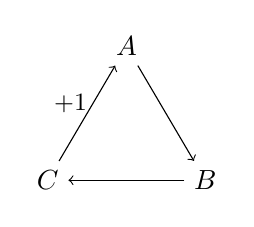
\begin{tikzpicture}
\node (C) at (0,0) {$C$};
\node (B) at (2,0) {$B$};
\node (A) at (1,1.7) {$A$};
\draw[->] 
(C) edge node[node font=\small,minimum height=2em,pos=0.5,yshift=-6pt,xshift=-6pt,above] {$+1$} (A)
(A) edge (B)
(B) edge (C);
\end{tikzpicture}\]
where the morphism labeled $+1$ acts as $C\to A[1]$; these diagrams are called \textbf{distinguished triangles}. A common alternative notation is
\[\begin{tikzcd}
A\ar[r]&B\ar[r]&C\ar[r,"+1"]&{}
\end{tikzcd}\]
Distinguished triangles are required to satisfy several axioms. Among them,
\[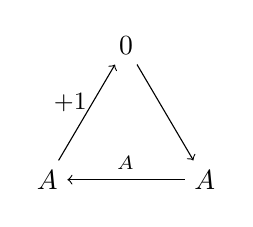
\begin{tikzpicture}
\node (C) at (0,0) {$A$};
\node (B) at (2,0) {$A$};
\node (A) at (1,1.7) {$0$};
\draw[->] 
(C) edge node[node font=\small,minimum height=2em,pos=0.5,yshift=-6pt,xshift=-6pt,above] {$+1$} (A)
(A) edge (B)
(B) edge node[above] {$\id_A$}(C);
\end{tikzpicture}\]
is required to be distinguished for every $A$; every morphism $\alpha:A\to B$ must be a side of a distinguished triangle; triangles isomorphic to a distinguished triangle (in the evident sense) must be distinguished; and distinguished triangles can be rotated:
\[\begin{tikzcd}
&A\ar[rd,"\alpha"]&\\
C\ar[ru,near start,"\gamma"]\ar[ru,near end,"+1"]&&B\ar[ll,"\beta"]
\end{tikzcd}\]
is distinguished if and only if
\[\begin{tikzcd}
&B\ar[rd,"\beta"]&\\
A[1]\ar[ru,near start,"-\alpha"]\ar[ru,near end,"+1"]&&C\ar[ll,"\gamma"]
\end{tikzcd}\]
is distinguished. There is more, including an infamous octahedral axiom (so named since a popular way to state it invokes an octahedral diagram). The reader will have no difficulties locating this information in the literature.\par
The category $\mathcal{K}(\mathcal{A})$ is triangulated: the translation functor is the basic shift of a complex, and distinguished triangles are those isomorphic to
\[\begin{tikzcd}
&L^\bullet\ar[rd,"\alpha"]&\\
MC(\alpha)^\bullet\ar[ru,"+1"]&&M^\bullet\ar[ll]
\end{tikzcd}\]
That is, the third vertex of a triangle with an assigned side $\alpha:L^\bullet\to M^\bullet$ is the mapping cone of $\alpha$, and the unlabeled sides are the natural cochain morphisms $M^\bullet\to MC(\alpha)^\bullet$, $MC(\alpha)^\bullet\to L[1]^\bullet$ studied in $\S4.1$.\par
It would be problematic to make the same choice in $\mathcal{C}(\mathcal{A})$, since while
\[\begin{tikzcd}
&0\ar[rd]&\\
L^\bullet\ar[ru,"+1"]&&L^\bullet\ar[ll,"\id_L"]
\end{tikzcd}\]
would be distinguished as needed, since $L^\bullet$ is the mapping cone of the zero-morphism $0\to L^\bullet$, the rotation of this triangle, i.e.,
\[\begin{tikzcd}
&L^\bullet\ar[rd,"\id_L"]&\\
0\ar[ru,"+1"]&&L^\bullet\ar[ll]
\end{tikzcd}\]
would not seem to be, since the mapping cone of the identity is not $0$. But the mapping cone of the identity is homotopically equivalent to $0$, so the rotated triangle is indeed distinguished in $\mathcal{K}(\mathcal{A})$, as it should be, according to the axioms. More generally, it is easy to see that if $\alpha:L^\bullet\to M^\bullet$ is a cochain morphism, so that we have a distinguished triangle,
\[\begin{tikzcd}
&L^\bullet\ar[rd,"\alpha"]&\\
MC(\alpha)^\bullet\ar[ru,"+1"]&&M^\bullet\ar[ll,"\beta"]
\end{tikzcd}\]
then the mapping cone of $\beta$ is in fact homotopy equivalent to $L[1]^\bullet$; the rotation
\[\begin{tikzcd}
&M^\bullet\ar[rd,"\beta"]&\\
L^\bullet\ar[ru,near end,"+1"]\ar[ru,near start,"-\alpha"]&&MC(\alpha)^\bullet\ar[ll]
\end{tikzcd}\]
is distinguished as required, as the reader should check.\par
Applying the cohomology functor to a distinguished triangle in K(A) yields an exact triangle: indeed, as we have just seen, we may assume that the triangle is of the form above. (up to isomorphism in $\mathcal{K}(\mathcal{A})$), and taking cohomology gives the exact triangle
\[\begin{tikzcd}
&H^\bullet(M^\bullet)\ar[rd]&\\
H^\bullet(L^\bullet)\ar[ru,"+1"]&&H^\bullet(MC(\alpha)^\bullet)\ar[ll]
\end{tikzcd}\]
In general, a \textbf{cohomological functor} on a triangulated category is an additive functor to an abelian category, mapping distinguished triangles to exact triangles and hence inducing long exact sequences. Thus, cohomology is a cohomological functor on $\mathcal{K}(\mathcal{A})$; this will not be surprising. The functors $\Hom(A,-)$ and $\Hom(-,A)$ (to $\mathsf{Ab}$) are cohomological functors on every triangulated category, for every object $A$.\par
Isomorphism in the derived category is a less stringent notion than in the homotopic category, so there are more distinguished triangles in $\mathcal{D}(\mathcal{A})$ than in $\mathcal{K}(\mathcal{A})$. For example, if
\[\begin{tikzcd}
0\ar[r]&L^\bullet\ar[r,"\alpha"]&M^\bullet\ar[r,"\beta"]&N^\bullet\ar[r]&0
\end{tikzcd}\]
is a short exact sequence, as above, there is in general no distinguished triangle
\[\begin{tikzcd}
&L^\bullet\ar[rd,"\alpha"]&\\
N^\bullet\ar[ru,near start,"\gamma"]\ar[ru,near end,"+1"]&&M^\bullet\ar[ll,"\beta"]
\end{tikzcd}\]
in $\mathcal{K}(\mathcal{A})$ (for any choice of $\gamma$): indeed, $N^\bullet$ need not be homotopically equivalent to $MC(\alpha)^\bullet$. But such triangles do exist in $\mathcal{D}(\mathcal{A})$! In fact, we are now well-equipped to make (better) sense of the mysterious remarks at the end of $\S3.4$. The special triangles
\[\begin{tikzcd}
&L^\bullet\ar[rd]&\\
N^\bullet\ar[ru,near start,"0"]\ar[ru,near end,"+1"]&&M^\bullet\ar[ll]
\end{tikzcd}\]
arising as in $\S3.4$ from a short exact sequence
\[\begin{tikzcd}
0\ar[r]&L^\bullet\ar[r,"\alpha"]&M^\bullet\ar[r,"\beta"]&N^\bullet\ar[r]&0
\end{tikzcd}\]
are not distinguished in $\mathcal{K}(\mathcal{A})$, and in general no replacement for the zero-morphism will fix this problem. On the other hand, the reader can now verify that there is a quasi-isomorphism $MC(\alpha)^\bullet\to N^\bullet$: this can be shown by computing explicitly another mapping cone and applying Corollary~\ref{MC exact iff quasi-iso}. Thus, in the derived category the standard distinguished triangle
\[\begin{tikzcd}
&L^\bullet\ar[rd,"\alpha"]&\\
MC(\alpha)^\bullet\ar[ru,"+1"]&&M^\bullet\ar[ll,"\beta"]
\end{tikzcd}\]
is isomorphic to a triangle
\[\begin{tikzcd}
&L^\bullet\ar[rd,"\alpha"]&\\
N^\bullet\ar[ru,near start,"\gamma"]\ar[ru,near end,"+1"]&&M^\bullet\ar[ll,"\beta"]
\end{tikzcd}\]
which is therefore distinguished in $\mathcal{D}(\mathcal{A})$. Applying the cohomology functor to this triangle directly gives the exact triangle
\[\begin{tikzcd}
&H^\bullet\ar[rd]&\\
H^\bullet(N^\bullet)\ar[ru,"+1"]&&H^\bullet(M^\bullet)\ar[ll]
\end{tikzcd}\]
expressing the long exact cohomology sequence as in $\S3.4$, without having to single out the $+1$ morphism for special consideration. In retrospect, the zero-morphism we insisted on using when folding special triangles in $\S3.4$ turns out to be an artifact: placing the triangle in the derived category shows that there is a more informed choice for this morphism. This choice is not available in $\mathcal{C}(\mathcal{A})$ and is not even in $\mathcal{K}(\mathcal{A})$, but it is available in $\mathcal{D}(\mathcal{A})$ and leads transparently to the long exact
sequence in cohomology.
\subsection{Spectral sequences}
\subsubsection{Exact couple}
Given that we were thinking about triangles a moment ago, the following construction may be helpful in appreciating the notion of spectral sequence. Let
\[\begin{tikzcd}
&A\ar[rd,"\alpha"]&\\
E\ar[ru,"\gamma"]&&A\ar[ll,"\beta"]
\end{tikzcd}\]
be an exact triangle\footnote{That is, $\im\alpha=\ker\beta$, $\im\beta=\ker\gamma$, and $\im\gamma=\ker\alpha$.} in an abelian category; we are placing no assumption on the degree of $\gamma$ (and indeed, we are not assuming we have defined a translation functor). Let $d:E\to E$ be the composition $\beta\circ\gamma$; since $\gamma\circ\beta=0$, we have
\[d\circ d=\beta\circ(\gamma\circ\beta)\circ\gamma=0.\]
Thus we can take the homology of $E$ with respect to $d$ and define
\[E'=\dfrac{\ker d}{\im d}\]
Further, we can let $A':=\im\alpha$ and let
\begin{itemize}
\item $\alpha':A'\to A'$ be the restriction of $\alpha$ to $A'$.
\item $\beta':A'\to E'$ be defined by $\beta'(\alpha(a)):=[\beta(a)]$.
\item $\gamma':E'\to A'$ be defined by $\gamma'([e]):=\gamma(e)$.
\end{itemize}
where $[e]$ denotes the class of $e\in E$ in $E'$. (Since $\beta\circ\gamma(e)=d(e)=0$, $\gamma(e)\in\ker\beta=\im\alpha=A'$.) 
We need to check the well-defiendness of $\beta'$ and $\gamma'$. These follow from the following arguments.
\begin{itemize}
\item From $d\circ\beta(a)=\beta\circ\gamma\circ\beta(a)=0$ we see $\beta(a)$ is a cocycle. Moreover, if $\alpha(a)=\alpha(\widetilde{a})$, then 
$a-\widetilde{a}=\gamma(e)$ for some $e\in E$. Thus
\[\beta(a)-\beta(\widetilde{a})=\beta\circ\beta(e)=d(e).\]
Therefore $[\beta(a)]=[\beta(\widetilde{a})]$ and thus $\beta'$ is well-defined.
\item For a cocycle $e\in E$ we have $d(e)=\beta\circ\gamma(e)=0$, so $\gamma(e)\in\ker\beta=\im\alpha$, so $\gamma'$ indeed maps $E'$ to $A'$. If $[e]=[\widetilde{e}]$ 
in $E'$, then $e-e'=d(\xi)$ for some $\xi\in E$. Then we see that
\[\gamma(e)-\gamma(e')=\gamma\circ d(\xi)=\gamma\circ\beta\circ\gamma(\xi)=0.\]
Therefore $\gamma$ is well-defined on the cohomology class.
\end{itemize}
The surprising part of our construction is that this new triangle is agian exact.
\begin{proposition}\label{der triangle}
The new triangle
\[\begin{tikzcd}
&A'\ar[rd,"\alpha'"]&\\
E'\ar[ru,"\gamma'"]&&A'\ar[ll,"\beta'"]
\end{tikzcd}\]
is again exact.
\end{proposition}
\begin{proof}
The composition of any two morphisms is obviously zero, so we only need to verify the other direction.\par
The exactness at the top $A'$ is clear: if $x\in\im\alpha$ satisfies $\alpha'(x)=0$, then $x\in\ker\alpha$, and there is $e\in E$ such that $\gamma(e)=x$. This means 
$\gamma'([e])=x$ provided $e$ is a cocycle. This is true because $d(e)=\beta\circ\gamma(e)=\beta(x)$ and $x\in\im\alpha=\ker\beta$.\par
For that of the right bottom $A'$, let $x\in\ker\beta'$, then there exists $a\in A$ such that 
\[\alpha(a)=x,\quad\beta'(x)=\beta(a)\in\im d.\]
Keep tracking, there is $e\in E$ such that $d(e)=\beta\circ\gamma(e)=\beta(a)$. This means $a-\gamma(e)\in\ker\beta=\im\alpha=A'$, and we find that 
$\alpha(a-\gamma(e))=\alpha(a)=x$.\par
Now we check $E'$. Suppose that $\gamma'([e])=0$ for some $[e]\in E'$. Then $\gamma(e)=0$ by our definition, and there is $a\in A$ such that $\beta(a)=e$. Choosing 
$\alpha(a)$ gives $\beta'(\alpha(a))=[e]$, as needed.
\end{proof}
The datum of an exact triangle as above is called an \textbf{exact couple}, which we find confusing since a triangle has three vertices (but it is true that only two 
objects are involved here); the new exact triangle (couple) obtained in Proposition~\ref{der triangle} is the \textbf{derived couple}, which we find even more confusing 
since there is no derived category or functor in sight. Exact couples arose in topology (they are due to W.Massey), and the terminology reflects their origin.\par
Of course we can turn the crank at will and get derived couple after derived couple: let $A_1=A$, $E_1=E$, etc., and inductively define $A_{i+1}:=A'_i, E_{i+1}:=E_i'$, 
etc. For example, $\beta_{i+1}$ is obtained by rewinding the morphism $\alpha$ a total of $i$ times and then applying the original morphism $\beta$: we can do this 
since $A_{i+1}$ is the image of $\alpha_i$; and $\gamma_{i+1}$ is induced by $\gamma_i$ on $E_{i+1}$.\par
Thus, one exact triangle produces a whole sequence of triangles and in particular a sequence of objects $E_i$, each endowed with a differential $d_i$, such that 
$E_{i+1}=\ker d_i/\im d_i$.
\begin{definition}
A \textbf{spectral sequence} $\{(E_i,d_i)\}_{i=1}^{\infty}$ is a sequence of objects $E_i$ and morphisms $d_i:E_i\to E_i$ in an abelian category, such that $d_i\circ d_i=0$ and $E_{i+1}\cong\ker d_i/\im d_i$.
\end{definition}
Thus, exact couples are a way to produce spectral sequences. There is a sense in which we can turn the crank infinitely many times; in fact, this can be done with any 
spectral sequence. To see this, let
\[Z_1=E_1,\quad B_1=0\]
so that $E_1\cong Z_1/B_1$; inductively, assume we have defined $Z_i\sub Z_1,B_i\sub Z_i$ so that $E_i\cong Z_i/B_i$, and let $\widebar{Z}_{i+1}=\ker d_i$, 
$\widebar{B}_{i+1}=\im d_i$; define $Z_{i+1}$, $B_{i+1}$ as the corresponding subobjects of $Z_i$ under the quotient. 
Then
\[E_{i+1}\cong\dfrac{\widebar{Z}_{i+1}}{\widebar{B}_{i+1}}\cong\dfrac{Z_i}{B_i}\]
realizing $E_{i+1}$ as a subquotient of $E_1$, and
\[B_1\sub\cdots\sub B_i\sub B_{i+1}\cdots\sub Z_{i+1}\sub Z_i\sub\cdots\sub Z_1.\]
Define
\[B_\infty=\bigcup_{i}B_i,\quad Z_\infty=\bigcap_iZ_i,\quad E_\infty=\dfrac{Z_\infty}{B_\infty}\]
This ultimate subquotient $E_\infty$ is the limit of the spectral sequence; it is common to say that the spectral sequence $E_r$ \textbf{abuts} to $E_\infty$. 
By definition, if $d_r=d_{r+1}=\cdots=0$, then $Z_\infty=Z_r$ and $B_\infty=B_r$, so that $E_\infty\cong E_r$; in this case we say that the sequence \textbf{collapses} 
at $E_r$.
\begin{proposition}\label{spectral seq from ext couple limit}
Let $(E_r,d_r)_{r=1}^{\infty}$ be a spectral sequence arising from an exact couple
\[\begin{tikzcd}
&A\ar[rd,"\alpha"]&\\
E\ar[ru,"\gamma"]&&A\ar[ll,"\beta"]
\end{tikzcd}\]
Then we have 
\[Z_{r+1}=\gamma^{-1}(\im\alpha^r),\quad B_{r+1}=\beta(\ker\alpha^r)\]
and therefore the limit $E_\infty$ is isomorphic to $\gamma^{-1}(\bigcap_r\im\alpha^r)/\beta(\bigcup_r\ker\alpha^r)$.
\end{proposition}
\begin{proof}
Let $[e]\in\widebar{Z}_{r+1}\sub E_r$, then $d_r([e])=\beta_r\circ\gamma_r([e])=0$. That is, $\gamma_r([e])\in\ker\beta_r=\im\alpha_r=\im\alpha^r$. Since $\gamma_r([e])=\gamma(e)$, 
we have $e\in\gamma^{-1}(\im\alpha^r)$. This gives one direction, the converse is obvious.\par
Now if $[e]\in\widebar{B}_{r+1}\sub E_r$, then $[e]=\beta_r\circ\gamma_r([e'])$ for some $[e']\in E_r$. From the definition of $\beta_r$, we have
\[[e]=\beta_r(\gamma_r([e']))=\beta(a)\text{ where }\alpha^{r-1}(a)=\gamma_r([e']).\]
Note that $\alpha\circ\alpha^{r-1}(a)=\alpha\circ\gamma_r([e'])=\alpha_r\circ\gamma_r([e'])=0$, so $a\in\ker\alpha^r$. This gives one direction, the other is trivial.
\end{proof}
\subsubsection{The spectral sequence of a double complex}
We will now see how a double complex gives rise to an exact couple and hence to a spectral sequence. This is a particular case of a useful mechanism producing an exact sequence from a filtration. A \textbf{descending filtration} of $M$ consists of a sequence of subobjects:
\[M\sups\cdots\sups M_m\sups M_{m+1}\sups\cdots\]
For example, the series of subgroups of a group $G$ are filtrations of $G$. If $M$ is an object of an abelian category, a filtration as above determines an associated graded object
\[\gr(M):=\bigoplus_m\gr(M)_m,\quad \gr(M)_m=\dfrac{M_m}{M_{m+1}}.\]
We will assume this is an object of the same category for simplicity, although this is not necessarily the case (abelian categories are not necessarily closed under
infinite direct sums); since only finitely many objects will be involved in any specific computation, this plays no role.\par
Start with a double complex $M^{\bullet,\bullet}$; we will assume that $M^{i,j}=0$ for $i<0$, $j<0$:
\[\begin{tikzcd}[column sep=1.6 em,row sep=1.6 em]
\vdots&\vdots&\vdots&\vdots&{}\\
M^{0,2}\ar[u,"\delta_v"]\ar[r,"d_h"]&M^{1,2}\ar[u,"\delta_v"]\ar[r,"d_h"]&M^{2,2}\ar[u,"\delta_v"]\ar[r,"d_h"]&M^{3,2}\ar[r,"d_h"]\ar[u,"\delta_v"]&\cdots\\
M^{0,1}\ar[r,"d_h"]\ar[u,"\delta_v"]&M^{1,1}\ar[u,"\delta_v"]\ar[r,"d_h"]\ar[u,"\delta_v"]&M^{2,1}\ar[u,"\delta_v"]\ar[r,"d_h"]&M^{3,1}\ar[u,"\delta_v"]\ar[r,"d_h"]&\cdots\\
M^{0,0}\ar[u,"\delta_v"]\ar[r,"d_h"]&M^{1,0}\ar[u,"\delta_v"]\ar[r,"d_h"]&M^{2,0}\ar[u,"\delta_v"]\ar[r,"d_h"]&M^{3,0}\ar[r,"d_h"]\ar[u,"\delta_v"]&\cdots
\end{tikzcd}\]
As always, zero-objects to the left and below the given part of the diagram are implicit; we are assuming (as in the definition) that the diagram anticommutes, so that 
the differential of the total complex $TC(M)^\bullet$ is simply $d_h+\delta_v$. Analogous results can be obtained if $M^{i,j}=0$ for $i>0$, $j>0$ and in fact under 
more relaxed hypotheses; such considerations are left to the reader.\par
Let $T^\bullet=TC(M)^\bullet$ denote the total complex: therefore, $T^k=\bigoplus_{i+j=k}M^{i,j}$. This complex admits (at least) two filtrations: a 
\textbf{horizontal filtration} and a \textbf{vertical filtration}. We will focus on the vertical one, and again it is understood that a parallel discussion would hold 
for the horizontal one. The vertical filtration $T^\bullet_m$ is defined by chopping off the terms to the left of a vertical bar $i=m$ in the diagram. That is, we set
\[T_m^k=\bigoplus_{\substack{i+j=k\atop i\geq m}}M^{i,j}\]
still with differential $d_h+\delta_v$. We will denote the corresponding graded object by $\gr(T)^\bullet$, to record the fact that this arises from the 
vertical filtration. Explicitly, the term of filtration degree $m$ in $\gr(T)^\bullet$ is 
\[\gr(T)^\bullet_m=T^\bullet_m/T^\bullet_{m+1}=\bigoplus_{i\geq m}M^{i,\bullet-i}/\bigoplus_{i\geq m+1}M^{i,\bullet-i}\cong M^{m,\bullet-m}.\]
That is, the filtration degree coincides with the vertical degree. The differential $d_h+\delta_v$ induces the differential $\delta_v$ on this graded piece, since 
$d_h$ is zero modulo the next piece of the filtration.\par
The filtration on $T^\bullet$ also determines a filtration on the cohomology of $T^\bullet$: we can take $H^\bullet(T^\bullet)_m$ to be the image in 
$H^\bullet(T^\bullet)$ of $H^\bullet(T^\bullet_m)$. Thus, we also have a graded object $\gr H^\bullet(T^\bullet)$ (Here the filtration degree is also the vertical 
degree). The relation between $H^\bullet(\gr(T)^\bullet)$ and $\gr H^\bullet(T^\bullet)$ is subtle: this relation is what spectral sequences will help us understand.\par 
The monomorphisms $T^\bullet_{m+1}\hookrightarrow T^\bullet_m$ define a monomorphism $\bigoplus_mT^\bullet_m\to\bigoplus_mT^\bullet_m$ as follows:
\[\begin{tikzcd}
\cdots\ar[draw=none]{r}[name=X, anchor=center,scale=1.5]{\oplus}&T^\bullet_{-2}\ar[draw=none]{r}[name=X, anchor=center,scale=1.5]{\oplus}&T^\bullet_{-1}
\ar[draw=none]{r}[name=X, anchor=center,scale=1.5]{\oplus}&T^\bullet_0\ar[draw=none]{r}[name=X, anchor=center,scale=1.5]{\oplus}&T^\bullet_1
\ar[draw=none]{r}[name=X, anchor=center,scale=1.5]{\oplus}&T^\bullet_2\ar[draw=none]{r}[name=X, anchor=center,scale=1.5]{\oplus}&\cdots\\
\cdots\ar[draw=none]{r}[name=X, anchor=center,scale=1.5]{\oplus}&T^\bullet_{-2}\ar[draw=none]{r}[name=X, anchor=center,scale=1.5]{\oplus}&T^\bullet_{-1}
\ar[draw=none]{r}[name=X, anchor=center,scale=1.5]{\oplus}\ar[lu]&T^\bullet_0\ar[draw=none]{r}[name=X, anchor=center,scale=1.5]{\oplus}\ar[lu]&T^\bullet_1
\ar[draw=none]{r}[name=X, anchor=center,scale=1.5]{\oplus}\ar[lu]&T^\bullet_2\ar[draw=none]{r}[name=X, anchor=center,scale=1.5]{\oplus}\ar[lu]&\cdots
\end{tikzcd}\]
This then gives rise to an exact sequence (recall that $T_m=T_0$ for $m<0$)
\begin{equation}\label{tot complex filtration}
\begin{tikzcd}
0\ar[r]&\bigoplus_mT^\bullet_m\ar[r]&\bigoplus_mT^\bullet_m\ar[r]&\gr(T)^\bullet\ar[r]&0
\end{tikzcd}
\end{equation}
which determines an exact triangle (the long exact sequence)
\[\begin{tikzcd}
&H^\bullet(\bigoplus_mT^\bullet_m)\ar[rd,"\alpha"]&\\
H^\bullet(\gr(T)^\bullet)\ar[ru,near start,"\gamma"]\ar[ru,near end, "+1"]&&H^\bullet(\bigoplus_mT^\bullet_m)\ar[ll,"\beta"]
\end{tikzcd}\]
Note that $\alpha$ decreases the filtration degree by $1$, leaving the cohomology degree $k$ unchanged; $\beta$ leaves both unchanged; and $\gamma$ increases both by 
$1$. This is particularly clear if one draws a small slice of the sequence $(\ref{tot complex filtration})$, sufficient to see the connecting morphism in action on a 
piece of given filtration and cohomology degrees:
\begin{equation}\label{spectral seq connecting map}
\begin{tikzcd}
0\ar[r]&T^{k+1}_{m+1}\ar[r]&T_m^{k+1}\ar[r]&\gr(T)^{k+1}_m\ar[r]&0\\
0\ar[r]&T^{k}_{m+1}\ar[u]\ar[r]&T_m^{k}\ar[u]\ar[r]&\gr(T)^{k}_m\ar[u]\ar[llu,dashed]\ar[r]&0
\end{tikzcd}
\end{equation}
Moreover, a little diagram chasing will lead us to the conclusion that $d_1=\beta\circ\gamma$ is the induced map of $d_h$ on $H^\bullet(\gr(T)^\bullet)$. In general, 
the differential $d_r=\beta_r\circ\gamma_r$ increases cohomology degree by $1$ and filtration degree by $r$.
\begin{definition}
The \textbf{spectral sequence of the double complex} $M^{\bullet,\bullet}$ (with respect to the vertical filtration) is the spectral sequence determined by this exact 
couple.
\end{definition}
We will denote this spectral sequence by $_{v}E$, with the absurdly positioned index $v$ recording that $_{v}E$ arises from the \textbf{vertical filtration}. The horizontal filtration
leads likewise to a spectral sequence $hE$.\par
All terms $_{v}E_r$ of the spectral sequence are subquotients of the first one, $_{v}E_1=H^\bullet(\gr(T)^\bullet)$.
\begin{theorem}\label{tot comp spectral}
Let $M^{\bullet,\bullet}$ be a double complex in an abelian category. Assume that $M^{i,j}=0$ for $i<0$, $j<0$, and let $T^\bullet$ be the total complex of $M^{\bullet,\bullet}$. Then, with notation as above, there exists a spectral sequence $\{(_{v}E_i,d_i)\}_i$ such that
\[_{v}E_1\cong H^\bullet(\gr(T)^\bullet),\quad _{v}E_\infty\cong \gr H^\bullet(T^\bullet).\]
\end{theorem}
\begin{proof}
The limit $_{v}E_{\infty}$ can be computed directly from the exact couple, as a subquotient of $_{v}E_{1}$: it is the quotient $Z_\infty/B_\infty$, where
\[Z_\infty=\gamma^{-1}(\bigcap_r\im\alpha^r),\quad B_\infty=\beta(\bigcup_r\ker\alpha^r).\]
The computation is streamlined by focusing on a specific degree $k$ for the cohomology and $m$ for the grading. The corresponding part in $_{v}E_1$ is 
$H^k(T^\bullet_m/T^\bullet_{m+1})$, and $\alpha$ acts as $H^k(T^\bullet_m)\to H^k(T^\bullet_{m-1})$. Note that we have 
\[H^k(T^\bullet_{m+r})=0,\quad H^k(T^\bullet_{m-r})=H^k(T^\bullet)\for r\gg 0\]
under our boundedness hypothesis. By these observations, the piece sent by $\alpha^r$ to $H^k(T^\bullet_m)$ is $0$ for $r\gg0$, and $\ker\alpha^r$ stabilizes to 
$\ker(H^k(T^\bullet_m)\to H^k(T^\bullet))$. These then imply
\[\big(\bigcap_r\im\alpha^r\big)\cap H^k(T_m^\bullet)=0,\quad \big(\bigcup_r\ker\alpha^r\big)\cap H^k(T_m^\bullet)=\ker(H^k(T^\bullet_m)\to H^k(T^\bullet)).\]
and thus
\begin{align}\label{tot comp spectral-1}
Z_\infty=\ker\gamma=\im\beta,\quad B_\infty=\beta(\bigoplus_m\ker(H^\bullet(T^\bullet_m)\to H^\bullet(T^\bullet)).
\end{align}
Denote by $\nu_m:H^\bullet(T^\bullet_m)\to H^\bullet(T^\bullet)$ the morphisms induced in cohomology by the monomorphisms $T^\bullet_m\to T^\bullet$ and by 
$\nu=\bigoplus\nu_m$ their direct sum, then we get from $(\ref{tot comp spectral-1})$ that
\[B_{\infty}=\beta(\bigoplus_m\ker\nu_m)=\beta(\ker(\bigoplus_m\nu_m)=\beta(\ker\nu).\]
We have morphisms
\[
\begin{tikzcd}
H^\bullet(\gr(T)^\bullet)&\bigoplus_mH^\bullet(T^\bullet_m)\ar[l,swap,"\beta"]\ar[r,"\nu"]&\bigoplus_mH^\bullet(T^\bullet)
\end{tikzcd}
\]
and we have obtained in Exercise~\ref{tow morphism im/im(ker) iso} that
\[_{v}E_\infty\cong\dfrac{\im\beta}{\beta(\ker\nu)}\cong\dfrac{\im\nu}{\nu(\ker\beta)}.\]
By the exactness of the original couple, we have
\[\ker\beta=\im\alpha=\bigoplus_m\im(H^\bullet(T^\bullet_{m+1})\to H^\bullet(T^\bullet_m)),\]
which implies that $\nu(\ker\beta)=\bigoplus_m\im\nu_{m+1}$ and therefore
\[_{v}E_\infty\cong\frac{\im\nu}{\nu(\ker\beta)}\cong\frac{\bigoplus_m\im\nu_m}{\bigoplus_m\im\nu_{m+1}}\cong\bigoplus_m\dfrac{\im\nu_m}{\im\nu_{m+1}}=\gr(H^\bullet(T^\bullet))\]
as stated.
\end{proof}
Theorem~\ref{tot comp spectral} is a substantial generalization of Theorems~\ref{tot comp exact} and ~\ref{tot reso}. To see that it implies Theorem~\ref{tot reso}, 
note that if the cohomology of each column $M^{i,\bullet}$ is concentrated in degree $0$, then $_{v}E_1$ is simply the complex
\begin{equation}\label{spectral seq eg}
\begin{tikzcd}
\cdots\ar[r]&0\ar[r]&H^0(M^{0,\bullet})\ar[r]&H^0(M^{1,\bullet})\ar[r]&H^0(M^{2,\bullet})\ar[r]&\cdots
\end{tikzcd}
\end{equation}
hence $_{v}E_2$ is the cohomology of this complex, and higher differentials of the spectral sequence are $0$ by degree considerations. It follows that the sequence collapses at $_{v}E_2$, and by Theorem~\ref{tot comp spectral} this says that $\gr(H^\bullet(T^\bullet))$ is isomorphic to the cohomology of $(\ref{spectral seq eg})$. In this case we clearly have $\gr(H^\bullet(T^\bullet))\cong H^\bullet(T^\bullet)$, so the conclusion reproduces the corresponding statement in Theorem~\ref{tot reso}. This is what is meant by the incantation \textit{by an immediate spectral sequence argument}.\par
This reasoning and other applications of the spectral sequence of a double complex are easier to understand if we make the following observation. View the original double complex
\[\begin{tikzcd}[column sep=1.0 em,row sep=1.2 em]
\vdots&\vdots&\vdots&\vdots&{}\\
M^{0,2}\ar[u]\ar[r,no head,dotted]&M^{1,2}\ar[u]\ar[r,no head,dotted]&M^{2,2}\ar[u]\ar[r,no head,dotted]&M^{3,2}\ar[r,no head,dotted]\ar[u]&\cdots\\
M^{0,1}\ar[r,no head,dotted]\ar[u]&M^{1,1}\ar[u]\ar[r,no head,dotted]\ar[u]&M^{2,1}\ar[u]\ar[r,no head,dotted]&M^{3,1}\ar[u]\ar[r,no head,dotted]&\cdots\\
M^{0,0}\ar[u]\ar[r,no head,dotted]&M^{1,0}\ar[u]\ar[r,no head,dotted]&M^{2,0}\ar[u]\ar[r,no head,dotted]&M^{3,0}\ar[r,no head,dotted]\ar[u]&\cdots
\end{tikzcd}\]
as an $E_0$ term in the sequence. The horizontal differentials are dotted out to highlight the fact that $_{v}E_1$ is obtained by taking the cohomology of the columns; this gives
\[\begin{tikzcd}[column sep=1.2 em,row sep=1.0 em]
H^2(T^\bullet_0/T^\bullet_1)\ar[r]&H^3(T^\bullet_1/T^\bullet_2)\ar[r]&H^4(T^\bullet_2/T^\bullet_3)\ar[r]&H^5(T^\bullet_3/T^\bullet_4)\ar[r]&\cdots\\
H^1(T^\bullet_0/T^\bullet_1)\ar[r]\ar[u,no head,dotted]&H^2(T^\bullet_1/T^\bullet_2)\ar[r]\ar[u,no head,dotted]&H^3(T^\bullet_2/T^\bullet_3)\ar[r]\ar[u,no head,dotted]&H^4(T^\bullet_3/T^\bullet_4)\ar[r]\ar[u,no head,dotted]&\cdots\\
H^0(T^\bullet_0/T^\bullet_1)\ar[r]\ar[u,no head,dotted]&H^1(T^\bullet_1/T^\bullet_2)\ar[r]\ar[u,no head,dotted]&H^2(T^\bullet_2/T^\bullet_3)\ar[r]\ar[u,no head,dotted]&H^3(T^\bullet_3/T^\bullet_4)\ar[r]\ar[u,no head,dotted]&\cdots
\end{tikzcd}\]
The differential of $_{v}E_1$ increases both the cohomological degree and the filtration degree by $1$, as indicated. To simplify dealing with the indices, it is common 
to assign degrees $(i,j)$ to the terms in $_{v}E_1$ according to the indices of the objects $M^{i,j}=M^{m,k-m}$ at which the cohomology is computed; that is, set
\[_{v}E_1^{i,j}=H^{i+j}(T^\bullet_i/T^\bullet_{i+1}).\]
Then the same array is drawn as
\[\begin{tikzcd}[column sep=1.2 em,row sep=1.0 em]
_{v}E_1^{0,2}\ar[r]&_{v}E_1^{1,2}\ar[r]&_{v}E_1^{2,2}\ar[r]&_{v}E_1^{3,2}\ar[r]&\cdots\\
_{v}E_1^{0,1}\ar[r]\ar[u,no head,dotted]&_{v}E_1^{1,1}\ar[r]\ar[u,no head,dotted]&_{v}E_1^{2,1}\ar[r]\ar[u,no head,dotted]&_{v}E_1^{3,1}\ar[r]\ar[u,no head,dotted]&\cdots\\
_{v}E_1^{0,0}\ar[r]\ar[u,no head,dotted]&_{v}E_1^{1,0}\ar[r]\ar[u,no head,dotted]&_{v}E_1^{2,0}\ar[r]\ar[u,no head,dotted]&_{v}E_1^{3,0}\ar[r]\ar[u,no head,dotted]&\cdots
\end{tikzcd}\]
The next term $_{v}E_2$ is obtained by taking the cohomology of $_{v}E_1$. Its differential
acts by increasing $m$ by $2$ and $k$ by $1$, that is, $i$ by $2$ and $j$ by $-1$. We can draw
this as
\[\begin{tikzcd}[column sep=1.2 em,row sep=1.2 em]
_{v}E_1^{0,2}\ar[r]\ar[rrd]&_{v}E_1^{1,2}\ar[r,no head,dotted]\ar[rrd]&_{v}E_1^{2,2}\ar[r,no head,dotted]\ar[rrd]&_{v}E_1^{3,2}\ar[r,no head,dotted]&\cdots\\
_{v}E_1^{0,1}\ar[r,no head,dotted]\ar[u,no head,dotted]\ar[rrd]&_{v}E_1^{1,1}\ar[r,no head,dotted]\ar[u,no head,dotted]\ar[rrd]&_{v}E_1^{2,1}\ar[r]\ar[u,no head,dotted]\ar[rrd]&_{v}E_1^{3,1}\ar[r,no head,dotted]\ar[u,no head,dotted]&\cdots\\
_{v}E_1^{0,0}\ar[r,no head,dotted]\ar[u,no head,dotted]&_{v}E_1^{1,0}\ar[r,no head,dotted]\ar[u,no head,dotted]&_{v}E_1^{2,0}\ar[r,no head,dotted]\ar[u,no head,dotted]&_{v}E_1^{3,0}\ar[r,no head,dotted]\ar[u,no head,dotted]&\cdots
\end{tikzcd}\]
In general, $_{v}E_r$ is the cohomology of $_{v}E_{r-1}$, and its differential increases $m$ by $r$ and $k$ by $1$; that is, $(i,j)\mapsto(i+r,j-(r-1))$. Pictorially, differentials at different stages act like this:
\[\includegraphics[scale=0.9]{pictures/spectral-seq-eg.pdf}\]
and so on.\par
\begin{remark}
For further application and a better understanding, we now give the intuitive construction of the differential $d_r$ in a diagram chasing viewpoint. First we consider 
$d_2$. Let $[\,\cdot\,]_r$ denote the cohomology class of $E_r$. For simplicity we will identify the preimage of $E_{r+1}$ in $E_r$, so that we have 
\[E_0\sups E_1\sups\cdots\sups E_r\sups E_{r+1}\sups\cdots.\]

Let $a\in E_2^{p,q}\sub E_0^{p,q}$, since $d_1$ is the induced map of $d_h$, we have $[d_h(a)]_1=0$. This means there exists $b\in E_0^{p,q}$ such that $-\delta_v(b)=d_h(a)$:
\[\begin{tikzcd}[column sep=1.0 em,row sep=1.0 em]
0&\\
a\ar[u]\ar[r]&{}\\
{}&b\ar[u]
\end{tikzcd}\]

In applying the map $\gamma_2$, we need to first pull $a$ back to a element of $T_{p+1}^\bullet$, and then apply the total differential 
$d_{tot}=d_h+\delta_v$. Since $a+b$ is a preimage of $a$, by our construction we have
\[\gamma_2(a)=\delta_v(a)+d_h(a)+\delta_v(b)+d_h(b)=d_h(b).\]
With this, since $d_h(b)$ can be viewed as an element of $T^\bullet_{p+2}$, by the definition of $\beta_r$ we get
\[d_2(a)=\beta_2(\gamma_2(a))=\beta_2(\alpha(d_h(b)))=[d_h(b)]_2.\]

In summary, the differential $d_2$ is represented by the following diagram
\[\begin{tikzcd}[column sep=1.0 em,row sep=1.0 em]
0&&\\
a\ar[u]\ar[r]&{}&{}\\
{}&b\ar[u]\ar[r]&d_h(b)
\end{tikzcd}\]
It can be easily showed that this definition is independent of the choice of $b$.\par
If moreover we have $d_2(a)=0$, then $[d_h(b)]_2=0$ and thus there exists an element $c\in E_1^{p+1,q-1}$ such that $d_1(c)=d_h(b)$. That is, we have
\[d_0(c)=\delta_v(c)=0,\quad d_1(c)=[d_h(c)]_1=[d_h(b)]_1.\] 
Combine this two equalities, we find that
\[d_1(b-c)=d_1(c)-d_1(b)=[d_h(c)-d_h(b)]_1=0,\quad d_0(b-c)=\delta_v(b)-\delta_v(c)=\delta_v(b)=-d_h(a),\]
so by replacing $b$ with $b_0:=b-c$, we can make $[d_h(b_0)]_1=0$, so there exists $b_1\in E_0^{p+2,q-1}$ such that $-\delta_v(b_1)=d_h(b_0)$. That is, we get the following diagram
\[\begin{tikzcd}[column sep=1.0 em,row sep=1.0 em]
0&&&\\
a\ar[u]\ar[r]&{}&{}&\\
{}&b_0\ar[u]\ar[r]&{}&\\
{}&{}&b_1\ar[u]\ar[r]&d_h(b_1)
\end{tikzcd}\]
By the same argument above, we see in this case, $d_3(a)$ is given by
\[d_3(a)=[d_h(b_1)]_3.\]

For a further step, we consider the condition $d_3(a)=0$. This means $[d_h(b_1)]_3=0$, so there exists $c_1\in E^{p+1,q-1}_2$ such that $d_2(c_1)=d_h(b_1)$. Therefore
\[d_0(c_1)=\delta_v(c_1)=0,\quad d_1(c_1)=[d_h(c_1)]_1=0,\quad d_2(c_1)=[d_h(b_1)]_2.\]
Unfolding the defintion of $d_2(c_1)$, there then exists $c_2\in E_0^{p+2,q-2}$ such that
\[d_h(c_1)=-\delta_v(c_2),\quad [d_h(c_2)]_2=[d_h(b_1)]_2.\]
These are summarized in the following:
\[\begin{tikzcd}[column sep=1.0 em,row sep=1.0 em]
0&&&\\
a\ar[u]\ar[r]&{}&{}&\\
{}&b_0\ar[u]\ar[r]&{}&\\
{}&{}&b_1\ar[u]\ar[r]&d_h(b_1)
\end{tikzcd}\quad\quad\quad\quad
\begin{tikzcd}[column sep=1.0 em,row sep=1.0 em]
0&&&\\
0\ar[u]\ar[r]&0&{}&\\
{}&c_1\ar[u]\ar[r]&{}&\\
{}&{}&c_2\ar[u]\ar[r]&d_h(c_2)
\end{tikzcd}\]
Now we have the following observations
\[\delta_v(b_0-c_1)=\delta_v(b_0)=-d_h(a),\quad d_2(b_0-c_1)=[d_h(b_1-c_2)]_2=0.\]
By applying the argument we made for $d_2$ on $b_0-c_1$, we can find a new diagram
\[\begin{tikzcd}[column sep=0.8 em,row sep=0.8 em]
0&&&\\
a\ar[u]\ar[r]&{}&{}&{}&{}\\
{}&b'_0\ar[u]\ar[r]&{}&{}&{}\\
{}&{}&b'_1\ar[u]\ar[r]&{}&{}\\
{}&{}&&b'_2\ar[u]\ar[r]&d_h(b'_2)
\end{tikzcd}\]
where $b_0':=b_0-c_1$ and $b'_2\in E_0$ is chosen to satisfy $-\delta_v(b'_2)=d_h(b'_1)$. Again, in this case we find
\[d_4(a)=[d_h(b_2')]_4.\]

Now we consider the converse. For an element $a\in E_0^{p,q}$, if there is a zig-zag of legnth $2$:
\[\begin{tikzcd}[column sep=1.0 em,row sep=1.0 em]
0&\\
a\ar[u]\ar[r]&{}\\
{}&b\ar[u]
\end{tikzcd}\]
then
\[d_1(a)=[d_h(a)]_1=[-\delta_v(b)]_1=0.\]
Similarly, if there is a zig-zag of legnth $3$ for $a$:
\[\begin{tikzcd}[column sep=1.0 em,row sep=1.0 em]
0&&&\\
a\ar[u]\ar[r]&{}&{}&\\
{}&b_0\ar[u]\ar[r]&{}&\\
{}&{}&b_1\ar[u]&
\end{tikzcd}\]
then
\[d_2(a)=[d_h(b_0)]_2=[[d_h(b_0)]_1]_2=[[-\delta_v(b_1)]_1]_2=0.\]
In general, if there is a zig-zag of legnth $r$ for $a$, then we can show $d_1(a)=d_2(a)=\cdots=d_{r-1}(a)=0$.\par
We say that an element $a$ in $E_0$ \textbf{lives to $\bm{E_{r}}$} if it represents a nontraivial cohomology class in $E_r$; equivalently, $a$ is a cocycle in $E_1,\dots,E_{r-1}$. From 
the discussion above we see that $a$ lives to $E_r$ if and only if it can be extended to a zig-zag of length $r$:
\[\begin{tikzcd}[column sep=1.0 em,row sep=1.0 em]
0&{}&{}&{}&{}&{}&{}\\
a\ar[u]\ar[r]&{}&{}&{}&{}&{}&{}\\
&b_1\ar[u]\ar[r]&{}&{}&{}&{}&{}\\
&&b_2\ar[u]\ar[r]&{}&{}&{}&{}\\
&&&\cdots\ar[u]\ar[r]&{}&{}&{}\\
&&&&b_{r-2}\ar[u]\ar[r]&{}&{}\\
&&&&&b_{r-1}\ar[u]\ar[r]&d_h(b_{r-1})
\end{tikzcd}\]
and the differential $d_r$ on $E_r$ is given by $d_h$ of the tail of the zig-zag:
\[d_r(a)=[d_h(b_{r-1})]_r.\]
\end{remark}
\subsubsection{The Spectral Sequence of a Filtered Complex}
More generally, we can consider the spectral sequence induced by a filtered complex. Let $M$ be a differential complex with differential operator $d$; i.e. $M$ has a 
grading $M=\bigoplus_{k\in\Z}M^k$ and $d:M^{k}\to M^{k+1}$ increases the degree by $1$. A \textbf{subcomplex} $M'$ of $M$ is a subobject such that $dM'\sub M'$. A 
sequence of subcomplexes
\[M=M_0\sups M_1\sups\cdots\sups M_i\sups\cdots\]
then makes $M$ into a filtered complex, with associated graded complex
\[\gr(M)=\bigoplus_{i=0}^{\infty}M_i/M_{i+1}.\]
For notational reasons we usually extend the filtration to negative indices by defining $M_i=M$ for $p<0$. Define $A=\bigoplus_{i\in\Z}M_i$, then the monomorphism $M_{i+1}\hookrightarrow M_i$ induces a map $A\to A$ whose cokernel is exactly $\gr(M)$. Therefore we have an exact sequence
\[\begin{tikzcd}
0\ar[r]&A\ar[r]&A\ar[r]&\gr(M)\ar[r]&0
\end{tikzcd}\]
which induces a long exact sequence of cohomology groups
\[\begin{tikzcd}
&H^\bullet(A)\ar[rd,"\alpha"]&\\
H^\bullet(\gr(M))\ar[ru,near start,"\gamma"]\ar[ru,near end,"+1"]&&H^\bullet(A)\ar[ll,"\beta"]
\end{tikzcd}\]
Since this diagram is an exact couple, it gives rise to a spectral seuqnece $\{(E_r,d_r)\}$.\par
Let $H_i$ be the image of $H(M_i)$ in $H(M)$, then there is 
a filtration of $H(M)$:
\[H(M)=H_0\sups H_1\sups \cdots\sups H_i\sups\cdots\]
making $H(M)$ into a filtered complex; this filtration is called the \textbf{induced filtration on $\bm{H(M)}$}.\par
To distinguish the grading degree $k$ from the filtration degree $i$, we will often call $k$ the \textbf{dimension}. Now the filtration $\{M_i\}$ on $M$ induces a 
filtration in each dimension: if $M_i^k=M^k\cap M_i$, then $\{M_i^k\}$ is a filtration on $M^k$. For the applications we have in mind, the filtration on $M$ need not 
have finite length. However, we can prove the following.
\begin{proposition}
Let $M=\bigoplus_{k\in\Z}M^k$ be a graded filtered complex with filtration $\{M_i\}$ and let $H(M)$ be the cohomology of $M$ with the induced filtration. Suppose 
for each degree $k$ the filtration $\{M^k_i\}$ has finite length. Then the short exact sequence
\[\begin{tikzcd}
0\ar[r]&\bigoplus_{i\in\Z}M_i\ar[r]&\bigoplus_{i\in\Z}M_i\ar[r]&\gr(M)\ar[r]&0
\end{tikzcd}\]
induces a spectral sequence which converges to $H^*(M)$.
\end{proposition}
\begin{proof}
The proof is similar to the case of double complex. We focuse on a specific degree $k$ for the cohomology and $i$ for the grading. The corresponding part in $E_1$ is 
$H^k(M_i/M_{i+1})$, and $\alpha$ acts as $H^k(M_i)\to H^k(M_{i-1})$. By the given condition, we have
\[H^k(M_{i+r})=0,\quad H^k(M_{i-r})=H^k(M)\for r\gg 0.\]
Therefore we have
\[\big(\bigcap_r\im\alpha^r\big)\cap H^k(M_i)=0,\quad \big(\bigcup_r\ker\alpha^r\big)\cap H^k(M_i)=\ker(H^k(M_i)\to H^k(M)).\]
and thus
\begin{align*}
Z_\infty=\ker\gamma=\im\beta,\quad B_\infty=\beta(\bigoplus_i\ker(H(M_i)\to H(M)).
\end{align*}
Denote by $\nu_i:H(M_i)\to H(M)$ the morphisms induced in cohomology by the monomorphisms $M_i\to M$ and by 
$\nu=\bigoplus\nu_i$ their direct sum, then we get
\[B_{\infty}=\beta(\bigoplus_i\ker\nu_i)=\beta(\ker(\bigoplus_i\nu_i)=\beta(\ker\nu).\]
The rest goes as Proposition~\ref{tot comp spectral}, and we omit it.
\end{proof}
\subsection{Exercise}
\begin{exercise}\label{tow morphism im/im(ker) iso}
Let $\lambda:M\to L$, $\nu:M\to N$ be morphisms in an abelian category:
\[\begin{tikzcd}
L&M\ar[l,swap,"\lambda"]\ar[r,"\nu"]&N
\end{tikzcd}\]
Prove that\footnote{Here $\lambda(\ker\nu)$ denotes the image of the restriction of $\lambda$ to the source of $\ker\nu$, etc.}
\[\dfrac{\im\lambda}{\lambda(\ker\nu)}\cong\dfrac{\im\nu}{\nu(\ker\lambda)}.\]
\end{exercise}
\begin{proof}
For a element $a\in\im\lambda$, define $\delta:\im\lambda\to\im\nu/\nu(\ker\lambda)$ by
\[\delta(a)=\nu(\ell)+\nu(\ker\lambda)\]
where $\ell\in M$ is a preimage of $a$. This is clearly well defined and we have
\[\ker\delta=\{a=\lambda(\ell):\nu(\ell)\in\nu(\ker\lambda)\}=\{a=\lambda(\ell):\ell\in\ker\nu+\ker\lambda\}=\lambda(\ker\nu).\]
The surjectivity of $\delta$ is clear.
\end{proof}
\begin{exercise}
Let $\alpha:L^\bullet\to M^\bullet$ be an isomorphism of cochain complexes. Prove that $MC(\alpha)^\bullet$ is homotopy equivalent to $0$.
\end{exercise}
\begin{proof}
Equivalently we show that the identity of $MC(\alpha)$ is homotopic to zero. Since $\alpha$ is an isomorphism, it has an inverse $\beta:M^\bullet\to L^\bullet$. Consider the diagram:
\[\begin{tikzcd}
&L^{i+1}\oplus M^i\ar[r,"d_{MC(\alpha)}^i"]\ar[ld,swap,"h^i"]\ar[d,"\id_{MC(\alpha)}"]&L^{i+2}\oplus M^{i+1}\ar[ld,"h^{i+1}"]\\
L^i\oplus M^{i-1}\ar[r,swap,"d_{MC(\alpha)}^{i-1}"]&L^{i+1}\oplus M^i&
\end{tikzcd}\]
where the homotopy $h$ is defined to be
\[h^i:(\ell,m)\mapsto(\beta^i(m),0)\]
then we check that
\[d_{MC(\alpha)}^{i-1}\circ h^i(\ell,m)=(-d^{i}_L\circ\beta(m),\beta^i(m))\]
\[h^{i+1}\circ d_{MC(\alpha)}^i(\ell,m)=(\ell+\beta^i\circ d_M^i(m),0)\]
since $\beta$ is a cochain morphism, we get 
\[\id_{MC(\alpha)}=d_{MC(\alpha)}^{i-1}\circ h^i+h^{i+1}\circ d_{MC(\alpha)}^i\]
as needed.
\end{proof}
\begin{exercise}
Let $\alpha:L^\bullet\to M^\bullet$ be a cochain morphism, and let $\beta:M^\bullet\to MC(\alpha)^\bullet$ be the natural morphism. Prove that $MC(\beta)^\bullet$ is homotopy equivalent to $L[1]^\bullet$.
\end{exercise}
\begin{proof}
The differential of $MC(\beta)$ acts as
\[\begin{tikzcd}
M^{i+1}\ar[draw=none]{d}[name=X, anchor=center,scale=1.5]{\oplus}\ar[r,"-d_M^{i+1}"]\ar[rdd,near start,"\id_M^{i+1}"]&M^{i+2}\ar[draw=none]{d}[name=X, anchor=center,scale=1.5]{\oplus}\\
L^{i+1}\ar[draw=none]{d}[name=X, anchor=center,scale=1.5]{\oplus}\ar[r,"-d_L^{i+1}"]\ar[rd,swap,"\alpha^{i+1}"]&L^{i+2}\ar[draw=none]{d}[name=X, anchor=center,scale=1.5]{\oplus}\\
M^i\ar[r,"d_M^i"]&M^{i+1}
\end{tikzcd}\]
Recall Exercise~\ref{map cyl homotopy equi}, we define the morphisms:
\[\rho:L[1]^i\to MC(\beta)^i,\quad \ell\mapsto(-\alpha(\ell),\ell,0)\]
\[\sigma:MC(\beta)^i\to L[1]^i,\quad (m',\ell,m)\mapsto\ell\]
since we have
\[d_{MC(\beta)}\circ\rho(\ell)=(d_M^i\circ\alpha(\ell),-d_L^{i+1}(\ell),0)=\rho\circ(-d_L^i)(\ell)\]
\[-d_L^{i+1}\circ\sigma(m',\ell,m)=-d_L^{i+1}(\ell)=\sigma\circ d_{MC(\beta)}(m',\ell,m)\]
$\sigma$ and $\rho$ are cohain morphisms. Clearly $\sigma\circ\rho=\id_{L[1]}$, and we have
\[(\id_{MC(\beta)}-\rho\circ\sigma)(m',\ell,m)=(m'+\alpha(\ell),0,m)\]
Picking $h^i:(m',\ell,m)\mapsto(m,0,0)$ gives a homotopy of $\rho\circ\sigma$ to $\id_{MC(\beta)}$, as the reader may check.
\end{proof}
\begin{exercise}
Let
\[\begin{tikzcd}
0\ar[r]&L^\bullet\ar[r,"\alpha"]&M^\bullet\ar[r,"\beta"]&N^\bullet\ar[r]&0
\end{tikzcd}\]
be a short exact sequence of cochain complexes on an abelian category.
\begin{itemize}
\item Prove that there is a cochain morphism $\gamma:MC(\alpha)^\bullet\to N^\bullet$ through which $\beta^\bullet:M^\bullet\to N^\bullet$ factors.
\item Prove that $MC(\gamma)^\bullet$ is an exact complex.
\item Conclude that $MC(\alpha)$ is quasi-isomorphic to $N^\bullet$.
\end{itemize}
\end{exercise}
\begin{proof}
\mbox{}
\begin{itemize}
\item Let $\gamma$ be the restriction of $MC(\alpha)^\bullet$ to $M^\bullet$ composing $\beta$, i.e.,
\[\gamma(\ell,m)=\beta(m)\]
it is easy to check this is a cochain morphism. From the definition we also have $\beta=\gamma\circ i$, where $i:M^\bullet\to MC(\alpha)$ is the inclusion, so $\beta$ factors though $\gamma$.
\item The differential of $MC(\gamma)$ acts as
\[\begin{tikzcd}
L^{i+2}\ar[draw=none]{d}[name=X, anchor=center,scale=1.5]{\oplus}\ar[r,"d_L^{i+2}"]\ar[rd,"\alpha^{i+2}"]&L^{i+3}\ar[rd,"\alpha^{i+3}"]\ar[r,"d_L^{i+3}"]\ar[draw=none]{d}[name=X, anchor=center,scale=1.5]{\oplus}&L^{i+4}\ar[draw=none]{d}[name=X, anchor=center,scale=1.5]{\oplus}\\
M^{i+1}\ar[draw=none]{d}[name=X, anchor=center,scale=1.5]{\oplus}\ar[r,"-d_M^{i+1}"]\ar[rd,"\beta^{i+1}"]&M^{i+2}\ar[rd,"\beta^{i+2}"]\ar[r,"-d_M^{i+2}"]\ar[draw=none]{d}[name=X, anchor=center,scale=1.5]{\oplus}&M^{i+3}\ar[draw=none]{d}[name=X, anchor=center,scale=1.5]{\oplus}\\
N^i\ar[r,"d_N^i"]&N^{i+1}\ar[r,"d_N^{i+1}"]&N^{i+2}
\end{tikzcd}\]
Now assume $(\ell^{i+3},m^{i+2},n^{i+1})\in\ker d_{MC(\gamma)}^{i+1}$. Then we have the equalities
\[\left\{\begin{array}{l}
d_L^{i+3}(\ell^{i+3})=0\\
\alpha^{i+3}(\ell^{i+3})-d_M^{i+2}(m^{i+2})=0\\
\beta^{i+2}(m^{i+2})+d_N^{i+1}(n^{i+1})=0
\end{array}\right. \]
The proof is similar to that of Theorem~\ref{tot comp exact}. First, let $n^i=0$. Since $\beta^{i+1}$ is epic, there is $m^{i+1}\in M^{i+1}$ such that $\beta^{i+1}(m^{i+1})=n^{i+1}$. Then
\[\beta^{i+2}\circ d_M^{i+1}
(m^{i+1})=d_N^{i+1}\circ\beta^{i+1}(m^{i+1})=d_N^{i+1}(n^{i+1})=-\beta^{i+2}(m^{i+2})\]
which gives $m^{i+2}=-d_M^{i+1}(m^{i+1})+x$, with $x\in\ker\beta^{i+2}=\im\alpha^{i+2}$. So $x=\alpha^{i+2}(\ell^{i+2})$ for some $\ell^{i+2}\in L^{i+2}$. Again,
\[\alpha^{i+3}\circ d_L^{i+2}(\ell^{i+2})=d_M^{i+2}\circ\alpha^{i+2}(\ell^{i+2})=d_M^{i+2}(m^{i+2}+d_M^{i+1}(m^{i+1}))=\alpha^{i+3}(\ell^{i+3})\]
Since $\alpha^{i+3}$ is monic, this gives $d_L^{i+2}(\ell^{i+2})=\ell^{i+3}$.
\item This follows from Corollary~\ref{MC exact iff quasi-iso}
\end{itemize}
\end{proof}
\begin{remark}
From the proof above, we can change the condition in Theorem~\ref{tot comp exact} so that only one direction of the double complex is bounded, but bounded above and below.
\end{remark}
\begin{exercise}
Let
\[\begin{tikzcd}
0\ar[r]&L^\bullet\ar[r,"\alpha"]&M^\bullet\ar[r,"\beta"]&N^\bullet\ar[r]&0
\end{tikzcd}\]
be a short exact sequence of cochain complexes on an abelian category $\mathcal{A}$. Prove that there is a morphism $N^\bullet\to L[1]^\bullet$ in the derived category $\mathcal{D}(\mathcal{A})$, inducing the connecting morphism $H^i(N^\bullet)\to H^{i+1}(L^\bullet)$ in cohomology.
\end{exercise}
\begin{proof}
In the derived category $\mathcal{D}(\mathcal{A})$, $MC(\alpha)$ is isomorphic to $N^\bullet$.
\end{proof}
\begin{exercise}
Let $_{v}E_r$ be the spectral sequence of a first-quadrant double complex from the vertical filtration. Prove that $_{v}E^{i,j}_r=_{v}E^{i,j}_\infty$ for $r>j+1$.
\end{exercise}
\begin{proof}
The differential $d_r$ maps indices $(i,j)\mapsto(i+r,j-(r-1))$. If $j-(r-1)<0$, this map woule be zero, hence the claim follows.
\end{proof}
\begin{exercise}
Let $\mathcal{A},\mathcal{B},\mathcal{C}$ be abelian categories, and let $\mathscr{F}:\mathcal{A}\to\mathcal{B}$, $\mathscr{G}:\mathcal{B}\to\mathcal{C}$ be additive 
functors. Assume that $\mathcal{A}$ and $\mathcal{B}$ have enough projectives, and that $\mathscr{F}$ sends projectives of $\mathcal{A}$ to $\mathscr{G}$-acyclic 
objects of $\mathcal{B}$, and that $\mathscr{G}$ is right-exact.\par
Let $A$ be an object of $\mathcal{A}$, and let 
\[\begin{tikzcd}
M^\bullet:&\cdots\ar[r]&M^{-2}\ar[r]&M^{-1}\ar[r]&M^0\ar[r]&0
\end{tikzcd}\]
be a projective resolution of $A$. Let $P^\bullet_{\mathscr{F}(M^\bullet)}$ be a Cartan-Eilenberg resolution of the complex $\mathscr{F}(M^\bullet)$. Consider the complex
\begin{equation}\label{two func reso-2}
\begin{tikzcd}
\cdots\ar[r]&\mathscr{G}(P^\bullet_{\mathscr{F}(M^{-2})})\ar[r]&\mathscr{G}(P^\bullet_{\mathscr{F}(M^{-1})})\ar[r]&\mathscr{G}(P^\bullet_{\mathscr{F}(M^{0})})\ar[r]&0
\end{tikzcd}
\end{equation}
obtained by applying $\mathscr{G}$ to $P^\bullet_{\mathscr{F}(M^\bullet)}$. \par
This is precisely the set-up of Exercise~\ref{two func exercise}. Now take the double complex associated with $(\ref{two func reso-2})$, and construct the spectral 
sequence corresponding to the horizontal filtration. Prove that the $E_2$ term of this sequence has terms
\[_{h}E^{p,q}_2=\mathcal{L}_p\mathscr{G}(\mathcal{L}_q\mathscr{F}(A))\]
This is the \textbf{Grothendieck spectral sequence}. Prove that it abuts to $\mathcal{L}_\bullet(\mathscr{G}\circ\mathscr{F})(A)$.
\end{exercise}
\begin{proof}
By Exercise~\ref{two func exercise} we know that this spectral sequence converges to $\mathcal{L}_n(\mathscr{G}\circ\mathscr{F})(A)$. Now we consider horizontal 
filtration. First, since $\mathscr{F}$ is right-exact, we have the follwing exact sequence:
\[\begin{tikzcd}
\cdots\ar[r]&\mathscr{F}(M^{-2})\ar[r]&\mathscr{F}(M^{-1})\ar[r]&\mathscr{F}(M^0)\ar[r]&\mathscr{F}(A)\ar[r]&0
\end{tikzcd}\]
Therefore we can construct a augmented Cartan-Eilenberg resolution of this augmented complex, which will be like
\[\begin{tikzcd}
{}&0&0&0&0&{}\\
\cdots\ar[r]&\mathscr{F}(M^{-2})\ar[r]\ar[u]&\mathscr{F}(M^{-1})\ar[r]\ar[u]&\mathscr{F}(M^0)\ar[r]\ar[u]&\mathscr{F}(A)\ar[r]\ar[u]&0\\
\cdots\ar[r]&P^0_{\mathscr{F}(M^{-2})}\ar[r]\ar[u]&P^0_{\mathscr{F}(M^{-1})}\ar[r]\ar[u]&P^0_{\mathscr{F}(M^{0})}\ar[r]\ar[u]&P^0\ar[r]\ar[u]&0\\
\cdots\ar[r]&P^1_{\mathscr{F}(M^{-2})}\ar[r]\ar[u]&P^1_{\mathscr{F}(M^{-1})}\ar[r]\ar[u]&P^1_{\mathscr{F}(M^{0})}\ar[r]\ar[u]&P^1\ar[r]\ar[u]&0\\
{}&\vdots\ar[u]&\vdots\ar[u]&\vdots\ar[u]&\vdots\ar[u]&{}
\end{tikzcd}\]
Since the original sequence is exact, this double complex is also exact. Using this fact and Exercise~\ref{two fuc reso}, we now compute the cohomology of each row in 
$\mathscr{G}(P^\bullet_{\mathscr{F}(M^\bullet)})$. We will get
\begin{equation}\label{G spectral seq-1}
\begin{tikzcd}
{}&0&0&0&{}\\
\cdots\ar[r]&\mathscr{G}(\mathcal{L}_2\mathscr{F}(A))\ar[r]\ar[u]&\mathscr{G}(\mathcal{L}_1\mathscr{F}(A))\ar[r]\ar[u]&\mathscr{G}(\mathcal{L}_0\mathscr{F}(A))\ar[r]\ar[u]&0\\
\cdots\ar[r]&\mathscr{G}(H^{2,0})\ar[r]\ar[u]&\mathscr{G}(H^{1,0})\ar[r]\ar[u]&\mathscr{G}(H^{0,0})\ar[r]\ar[u]&0\\
\cdots\ar[r]&\mathscr{G}(H^{2,1})\ar[r]\ar[u]&\mathscr{G}(H^{1,1})\ar[r]\ar[u]&\mathscr{G}(H^{0,1})\ar[r]\ar[u]&0\\
{}&\vdots\ar[u]&\vdots\ar[u]&\vdots\ar[u]&
\end{tikzcd}
\end{equation}
By the right-exactness of $\mathscr{G}$, each column is exact. Moreover, since each $H^{i,j}$ can be chosen to be projective, the $p$-th column of $(\ref{G spectral seq-1})$ 
then computes $\mathcal{L}_\bullet\mathscr{G}(\mathcal{L}_p\mathscr{F}(A))$. This is the $E_2$ page.
\end{proof}